\def\GRAPHPATH{graphics}

\ifdefined\HANDOUT
  \documentclass[handout,aspectratio=1610,dvipsnames]{beamer}
  \def\GRAPHPATH{graphics}
\else
  \documentclass[aspectratio=1610,dvipsnames]{beamer}
\fi

\usepackage[ngerman]{babel}
\usepackage{amsmath}
\usepackage{amssymb}
\usepackage{ifthen}
\usepackage{color}
\usepackage{colortbl}
\usepackage{textcomp}
\usepackage{multirow}
\usepackage{nicefrac}
\usepackage{multicol}
\usepackage{langsci-gb4e}
\usepackage{verbatim}
\usepackage{cancel}
\usepackage{graphicx}
\usepackage{hyperref}
\usepackage{verbatim}
\usepackage{boxedminipage}
\usepackage{adjustbox}
\usepackage{rotating}
\usepackage{booktabs}
\usepackage{bbding}
\usepackage{pifont}
\usepackage{multicol}
\usepackage{stmaryrd}
\usepackage{FiraSans}
\usepackage{soul}
\usepackage{tikz}
\usepackage{array}
\usepackage{xstring}
\usepackage{epic,ecltree,eepic}
\usepackage{pstricks}
\usepackage{tree-dvips}
\usepackage{xyling}
\usepackage{setspace}
\usepackage{datatool,xparse}
\usepackage{calc}
\usepackage{fontawesome}

\usetikzlibrary{calc,decorations.pathmorphing,tikzmark,positioning,chains,trees,graphs,shapes,shadows,arrows}

\renewcommand\tikzmark[2]{%
  \tikz[remember picture,baseline=(chain-1.base),start chain] \node[on chain,inner sep=2pt,outer sep=0] (#1){#2};%
}

\newcommand\link[2]{%
  \begin{tikzpicture}[remember picture, overlay, >=stealth, shift={(0,0)}]
    \draw[-] (#1) --++(0,-12pt) -| (#2);
   \end{tikzpicture}%
}


\makeatletter
\g@addto@macro{\endtabular}{\rowfont{}}% Clear row font
\makeatother
\newcommand{\rowfonttype}{}% Current row font
\newcommand{\rowfont}[1]{% Set current row font
   \gdef\rowfonttype{#1}#1%
}
\newcolumntype{L}{>{\rowfonttype}l}


\usepackage{tikz-qtree}
\usepackage[linguistics]{forest}
\usepackage[maxbibnames=99,
  maxcitenames=2,
  uniquelist=false,
  backend=biber,
  doi=false,
  url=false,
  isbn=false,
  bibstyle=biblatex-sp-unified,
  citestyle=sp-authoryear-comp]{biblatex}

% Biblatex ============================================================

\addbibresource{rs.bib}

% Colors ==============================================================

\ifdefined\HANDOUT
  \definecolor{grau}{rgb}{0.5,0.5,0.5}
  \definecolor{lg}{rgb}{0.8,0.8,0.8}
  \definecolor{trueblue}{rgb}{0.3,0.3,1}
  \definecolor{ltb}{rgb}{0.8,0.8,1}
  \definecolor{lgr}{rgb}{0.5,1,0.5}
  \definecolor{orongsch}{RGB}{255,165,0}
  \definecolor{gruen}{rgb}{0,0.4,0}
  \definecolor{rot}{rgb}{0.7,0.2,0.0}
  \definecolor{tuerkis}{RGB}{63,136,143}
  \definecolor{braun}{RGB}{108,71,65}
  \definecolor{blaw}{rgb}{0,0,0.9}
\else
  \definecolor{grau}{rgb}{0.7,0.7,0.7}
  \definecolor{lg}{rgb}{0.9,0.9,0.9}
  \definecolor{trueblue}{rgb}{0.8,0.8,1}
  \definecolor{ltb}{rgb}{0.9,0.9,1}
  \definecolor{lgr}{rgb}{0.7,1,0.7}
  \definecolor{orongsch}{RGB}{255,200,100}
  \definecolor{gruen}{RGB}{0,230,0}
  \definecolor{rot}{RGB}{255,155,100}
  \definecolor{tuerkis}{RGB}{150,205,205}
  \definecolor{braun}{RGB}{140,120,115}
  \definecolor{blaw}{rgb}{0,0,0.9}
\fi

\newcommand{\gruen}[1]{\textcolor{gruen}{#1}}
\newcommand{\blaw}[1]{\textcolor{blaw}{#1}}
\newcommand{\rot}[1]{\textcolor{rot}{#1}}
\newcommand{\blau}[1]{\textcolor{trueblue}{#1}}
\newcommand{\orongsch}[1]{\textcolor{orongsch}{#1}}
\newcommand{\grau}[1]{\textcolor{grau}{#1}}
\newcommand{\whyte}[1]{\textcolor{white}{#1}}
\newcommand{\tuerkis}[1]{\textcolor{tuerkis}{#1}}
\newcommand{\braun}[1]{\textcolor{braun}{#1}}

% Newcommands =========================================================

\newcommand{\Dim}{\cellcolor{lg}}
\newcommand{\Dimblue}{\cellcolor{ltb}}
\newcommand{\Dimgreen}{\cellcolor{lgr}}
\newcommand{\Sub}[1]{\ensuremath{_{\text{#1}}}}
\newcommand{\Up}[1]{\ensuremath{^{\text{#1}}}}
\newcommand{\UpSub}[2]{\ensuremath{^{\text{#1}}_{\text{#2}}}}
\newcommand{\Spur}[1]{t\Sub{#1}}
\newcommand{\Ti}{\Spur{1}}
\newcommand{\Tii}{\Spur{2}}
\newcommand{\Tiii}{\Spur{3}}
\newcommand{\Tiv}{\Spur{4}}
\newcommand{\Ck}{\CheckmarkBold}
\newcommand{\Fl}{\XSolidBrush}
\newcommand{\xxx}{\hspaceThis{[}}
\newcommand{\zB}{z.\,B.\ }
\newcommand{\down}[1]{\ensuremath{\mathrm{#1}}}
\newcommand{\Zeile}{\vspace{\baselineskip}}
\newcommand{\Halbzeile}{\vspace{0.5\baselineskip}}
\newcommand{\Viertelzeile}{\vspace{0.25\baselineskip}}
\newcommand{\KTArr}[1]{\ding{222}~\fbox{#1}~\ding{222}}
\newcommand{\Ast}{*}
\newcommand{\SL}{\ensuremath{\llbracket}}
\newcommand{\SR}{\ensuremath{\rrbracket}}
\def\lspbottomrule{\bottomrule}
\def\lsptoprule{\toprule}
\newcommand{\Sw}[1]{\begin{sideways}#1\end{sideways}}
\newcommand{\Lab}{\ensuremath{\langle}}
\newcommand{\Rab}{\ensuremath{\rangle}}
\newcommand{\AbUmlautBreaker}{}
\ifdefined\HANDOUT
  \renewcommand{\AbUmlautBreaker}{\ /}
\fi
\newcommand{\LocStrutGrph}{\hspace{0.1\textwidth}}
\newcommand{\Nono}{---}

\newcommand{\Bewegtes}[1]{\ensuremath{_{\textrm{#1}}}}
\newcommand{\ORi}{\Bewegtes{1}}
\newcommand{\ORii}{\Bewegtes{2}}
\newcommand{\ORiii}{\Bewegtes{3}}
\newcommand{\ORiv}{\Bewegtes{4}}
\newcommand{\ORv}{\Bewegtes{5}}


\newcommand{\den}[1]{{$\llbracket${}#1$\rrbracket$}}
\newcommand{\dem}[1]{{\llbracket{}#1\rrbracket}}

% Beamer ==============================================================

\usetheme[hideothersubsections]{Boadilla}

\ifdefined\HANDOUT
  \usecolortheme{whale}
\else
  \usecolortheme{magpie}
\fi

\renewcommand<>{\rot}[1]{%
  \alt#2{\beameroriginal{\rot}{#1}}{#1}%
}
\renewcommand<>{\blau}[1]{%
  \alt#2{\beameroriginal{\blau}{#1}}{#1}%
}
\renewcommand<>{\orongsch}[1]{%
  \alt#2{\beameroriginal{\orongsch}{#1}}{#1}%
}
\renewcommand<>{\gruen}[1]{%
  \alt#2{\beameroriginal{\gruen}{#1}}{#1}%
}

\setbeamercolor{alerted text}{fg=trueblue}

\newcounter{lastpagemainpart}

\resetcounteronoverlays{exx}

\AtBeginSection[]{
  \begingroup
  \setbeamertemplate{navigation symbols}{}
  \begin{frame}[noframenumbering,plain]
  \vfill
  \centering
  \begin{beamercolorbox}[sep=8pt,center,shadow=true,rounded=true]{title}
    \usebeamerfont{title}\insertsectionhead\par%
  \end{beamercolorbox}
  \vfill
  \end{frame}
  \endgroup
}

\setbeamertemplate{itemize item}[circle]
\setbeamertemplate{enumerate item}[square]


\makeatother
\setbeamertemplate{footline}
{
  \leavevmode%
  \hbox{%
  \begin{beamercolorbox}[wd=.4\paperwidth,ht=2.25ex,dp=1ex,center]{author in head/foot}%
    \usebeamerfont{author in head/foot}\insertshortauthor
  \end{beamercolorbox}%
  \begin{beamercolorbox}[wd=.6\paperwidth,ht=2.25ex,dp=1ex,center]{title in head/foot}%
    \usebeamerfont{title in head/foot}\insertshorttitle\hspace*{3em}
    \insertframenumber{} / \inserttotalframenumber\hspace*{1ex}
  \end{beamercolorbox}}%
  \vskip0pt%
}
\makeatletter
\setbeamertemplate{navigation symbols}{}


% Tikz ================================================================

\usetikzlibrary{positioning,arrows,cd}
\tikzset{>=latex}

% Forest

\forestset{
  Ephr/.style={draw, ellipse, thick, inner sep=2pt},
  Eobl/.style={draw, rounded corners, inner sep=5pt},
  Eopt/.style={draw, rounded corners, densely dashed, inner sep=5pt},
  Erec/.style={draw, rounded corners, double, inner sep=5pt},
  Eoptrec/.style={draw, rounded corners, densely dashed, double, inner sep=5pt},
  Ehd/.style={rounded corners, fill=gray, inner sep=5pt,
    delay={content=\whyte{##1}}
  },
  Emult/.style={for children={no edge}, for tree={l sep=0pt}},
  phrasenschema/.style={for tree={l sep=2em, s sep=2em}},
  decide/.style={draw, chamfered rectangle, inner sep=2pt},
  finall/.style={rounded corners, fill=gray, text=white},
  intrme/.style={draw, rounded corners},
  yes/.style={edge label={node[near end, above, sloped, font=\scriptsize]{Ja}}},
  no/.style={edge label={node[near end, above, sloped, font=\scriptsize]{Nein}}},
  sake/.style={tier=preterminal},
  ake/.style={
    tier=preterminal
    },
}

\tikzset{
    invisible/.style={opacity=0,text opacity=0},
    visible on/.style={alt=#1{}{invisible}},
    alt/.code args={<#1>#2#3}{%
      \alt<#1>{\pgfkeysalso{#2}}{\pgfkeysalso{#3}}
    },
}

\forestset{
  visible on/.style={
    for tree={
      /tikz/visible on={#1},
      edge+={/tikz/visible on={#1}}}}}

\useforestlibrary{edges}

\forestset{
  narroof/.style={roof, inner xsep=-0.25em, rounded corners},
  forky/.style={forked edge, fork sep-=7.5pt},
  bluetree/.style={for tree={trueblue}, for children={edge=trueblue}},
  orongschtree/.style={for tree={orongsch}, for children={edge=orongsch}},
  rottree/.style={for tree={rot}, for children={edge=rot}},
  gruentree/.style={for tree={gruen}, for children={edge=gruen}},
  tuerkistree/.style={for tree={tuerkis}, for children={edge=tuerkis}},
  brauntree/.style={for tree={braun}, for children={edge=braun}},
  grautree/.style={for tree={grau}, for children={edge=grau}}, 
  gruennode/.style={gruen, edge=gruen},
  graunode/.style={grau, edge=grau},
}


% Drawing sonority diagrams =========================================== 

\makeatletter

\long\def\ifnodedefined#1#2#3{%
  \@ifundefined{pgf@sh@ns@#1}{#3}{#2}}

\newcommand\aeundefinenode[1]{%
  \expandafter\ifx\csname pgf@sh@ns@#1\endcsname\relax
  \else
    \typeout{Undefining node "#1"}%
    \global\expandafter\let\csname pgf@sh@ns@#1\endcsname\relax
  \fi
}

\newcommand\aeundefinethesenodes[1]{%
  \foreach \myn  in {#1}
    {%
      \ifnodedefined{\myn}{%
      \expandafter\aeundefinenode\expandafter{\myn}%
    }{}
    }%
}

\newcommand\aeundefinenumericnodes{%
  \foreach \myn in {1,2,...,50}
    {%
      \ifnodedefined{\myn}{%
      \expandafter\aeundefinenode\expandafter{\myn}%
    }{}
    }%
}
\makeatother

\newcommand{\plo}{0}
\newcommand{\fri}{0.5}
\newcommand{\nas}{1}
\newcommand{\liq}{1.5}
\newcommand{\vok}{2}

% Save text.
\newcommand{\lastsaved}{}
\newcommand{\textsave}[1]{\gdef\lastsaved{#1}#1}

\newcommand{\SonDiag}[2][0]{%
  \begin{tikzpicture}
    \textsave{.}
    \tikzset{
      normalseg/.style={fill=white},
      extrasyll/.style={circle, draw, fill=white},
      sylljoint/.style={diamond, draw, fill=white}
    }
    \node at (0,\plo) {P};
    \node at (0,\fri) {F};
    \node at (0,\nas) {N};
    \node at (0,\liq) {L};
    \node at (0,\vok) {V};

    % Draw the helper lines if required.
    \ifthenelse{\equal{#1}{0}}{}{%
      \foreach \y in {\plo, \fri, \nas, \liq,\vok} {%
	\draw [dotted, |-|] (0.25, \y) -- (#1.75, \y);
      }
    }

    \foreach [count=\x from 1, remember=\x as \lastx] \p / \y / \g in #2 {
      \ifthenelse{\equal{\y}{-1}}{\textsave{.}}{%

	% Draw the node, either plain, as Silbenbgelenk, or as extrasyllabic.
        \ifthenelse{\equal{\g}{1}}{%
	  \node (\x) [sylljoint] at (\x, \y) {\p};
	}{%
	  \ifthenelse{\equal{\g}{2}}{%
	    \node (\x) [extrasyll] at (\x, \y) {\p};
	  }{%
	    \node (\x) [normalseg] at (\x, \y) {\p};
	  }
	}

	% Draw the connection unless the previous node was not or was empty.
	\ifthenelse{\NOT\equal{\lastsaved}{.}}{%
	  \draw [->] (\lastx) to (\x);
	}{}
	\textsave{1}
      }
    }
    \aeundefinenumericnodes
  \end{tikzpicture}
}


\setbeamertemplate{navigation symbols}{}
\setbeamertemplate{section in toc}[circle]
\setbeamertemplate{subsection in toc}[square]
\setbeamertemplate{subsubsection in toc}[triangle]

\setbeamerfont{section in toc}{size=\tiny}
\setbeamerfont{subsection in toc}{size=\tiny}
\setbeamerfont{subsubsection in toc}{size=\tiny}




\ifdefined\TITLE
  \title[Semantik | \letterssub{\TITLE}]{Formale Semantik\\\letterssub{\TITLE}}
\else
  \title[Formale Semantik]{Formale Semantik}
\fi

\author{Roland Schäfer}
\institute[FSU Jena]{Institut für Germanistische Sprachwissenschaft\\Friedrich-Schiller-Universität Jena}
\date[\today]{\grau{Stets aktuelle Fassungen: \url{https://github.com/rsling/VL-Semantik}}}

\begin{document}

\begingroup
  \setbeamertemplate{navigation symbols}{}
  \begin{frame}[noframenumbering,plain,allowframebreaks]
   \titlepage
  \end{frame}
  \begin{frame}{Inhalt}
    \centering
    \begin{minipage}{0.8\textwidth}
        \begin{multicols}{2}
          \tableofcontents
        \end{multicols}
    \end{minipage}
  \end{frame}
\endgroup

\ifdefined\TITLE
  \input{includes/\TITLE}
\else
  \section[Inferenz und Bedeutung]{Inferenz und Bedeutung}
  \let\woopsi\section\let\section\subsection\let\subsection\subsubsection
  
\section{Organisation}

\begin{frame}
  {Literatur | Einführungen}
  \onslide<+->
  \onslide<+->
  Die folgenden drei Bücher sind die Grundlage des Seminars:\\
  \Zeile
  \begin{itemize}[<+->]
    \item \alert{\citet{ChierchiaMcconnellginet2000}} | GB-orientiert, nur die Kapitel von Chierchia
    \item \alert{\citet{DowtyEa1981}} | Tolle Montague-Einführung von seinen Schülern
    \item \alert{\citet{ParteeEa1990}} | Wichtige Grundlagen (Algebra, Logik), viele Druckfehler
  \end{itemize}
  \onslide<+->
  \centering 
  \large
  \Zeile
  \rot{Die auf den Folien angegebenen Teile dieser Bücher sollten\\
  für die Prüfungen durchgearbeitet werden. Das heißt natürlich nicht,\\
  dass Sie alles auswendig lernen sollen. Die Folien geben die Hinweise,\\
  was aus den Texten wichtig ist, sind aber nicht selbsterklärend.}
\end{frame}

\begin{frame}
  {Literatur | weitere Empfehlungen}
  \onslide<+->
  \begin{itemize}[<+->]
    \item \alert{\citet{Bucher1998}} | Lesbare Logik-Einführung auf Deutsch
    \item \alert{\citet{Carpenter1997}} | Prima Hardcore-Einführung mit Kategorialgrammatik
    \item \alert{\citet{Gutzmann2019}} | Aktuelle Einführung auf Deutsch
  \end{itemize}
\end{frame}


\begin{frame}
  {Seminarverlauf}
  \onslide<+->
  \begin{enumerate}[<+->]\Lf\scriptsize
    \item \alert{9.10.2023} Diskussion: Wie schlussfolgern wir? Wie hängen unser Schlussfolgerungen mit Semantik zusammen?
    \item \alert{26.10.2023} Referentielle Semantik (Folien 2)
    \item \alert{02.11.2023} Referentielle Semantik (Folien 2) II
    \item \alert{09.11.2023} Mengen- und Funktionstheorie (Folien 3)
    \item[\rule{1.2em}{1.2em}] \raisebox{2pt}{\grau{16.11.2023 Ausfall wegen Dienstreise}}
    \item \alert{23.11.2023} Aussagenlogik (Folien 4)
    \item \alert{30.11.2023} Prädikatenlogik (Folien 5)
    \item \alert{07.12.2023} Quantifikation und modelltheoretische Semantik (Folien 6)
    \item \alert{14.12.2023} Getypte λ-Sprachen höherer Ordnung (Folien 7)
    \item \alert{21.12.2023} Intensionalität (Folien 8)
    \item[\rule{1.2em}{1.2em}] \raisebox{2pt}{\grau{28.12.2023 Weihnachtsferien}}
    \item[\rule{1.2em}{1.2em}] \raisebox{2pt}{\grau{04.01.2024 Weihnachtsferien}}
    \item \alert{11.01.2024} Tempus und Modalität (Folien 9)
    \item \alert{18.01.2024} Montagues intensionale Logik (Folien 10)
    \item \alert{25.01.2024} Lektüre 
    \item \alert{01.02.2024} Lektüre
    \item \alert{08.02.2024} Lektüre
  \end{enumerate}
\end{frame}

\begin{frame}
  {Semesterplan und Lernen für die Prüfung}
  \onslide<+->
  \onslide<+->
  \centering 
  \alert{\large Hinweis in eigener Sache}\\
  \Halbzeile
  \begin{itemize}[<+->]
    \item Vermutlich ist der Plan bis Weihnachten zu ambitioniert.
    \item Die Wochen 4 und 5 könnten länger dauern, Woche 7 ebenfalls.
    \item Dann ändert sich der Plan noch, eventuell fliegen Artikel am Ende raus.
  \end{itemize}
  \Zeile
  \onslide<+->
  \alert{\large Hinweis zum Lernen}\\
  \Halbzeile
  \begin{itemize}[<+->]
    \item Wir haben es hier mir anspruchsvollem Material zu tun.
    \item Nur so ergibt meiner Meinung nach formale Semantik Sinn,\\
      und irgendwelche weichgespülten Einführungen sind grob fahrlässig.
    \item Daher gilt aber: Wenn Sie nicht von Anfang an lernen,\\
      wird es sehr wahrscheinlich gegen Ende sehr schwierig!
  \end{itemize}
\end{frame}

\begin{frame}
  {Prüfungen}
  \onslide<+->
  \onslide<+->
  Einheitlicher Inhalt für alle Modul- und Examensprüfungen:\\
  \Zeile
  \begin{enumerate}[<+->]
    \item eine oder zwei inhaltlichen Fragen zu den Themen der \textit{Sprachphilosophie}\\
      \grau{\footnotesize Die Liste der relevanten Texte wird rechtzeitig vor den Prüfungen eingeschränkt.}
    \item eine Logik-Aufgabe (natürliche Deduktion) -- \alert{außer in mündlichen Prüfungen}
    \item eine Semantik-Aufgabe (kompositionale Modellierung eines Satzes)
  \end{enumerate}
  \Zeile
  \onslide<+->
  \grau{Hausarbeiten nach Absprache.}
\end{frame}

\begin{frame}
  {Die unausweichliche Frage nach ein paar Wochen \visible<2->{| \rot{WTF???}}}
  \onslide<+->
  \onslide<+->
  \onslide<+->
  "`Wozu brauchen wir das denn?"'\\
  \Halbzeile
  \begin{itemize}[<+->]
    \item Nicht zu leugnende \alert{logische Eigenschaften von Sprache}
    \item Kleiner Einblick in deren \alert{technisch sehr aufwendige Beschreibung}
      \Halbzeile
    \item Wichtige Lernziele
      \begin{itemize}[<+->]
        \item Realistische Einschätzung \alert{eigener semantischer Intuitionen}
        \item Erkennen der \alert{Grenzen der Möglichkeiten von Logik} in der Analyse von Sprache
        \item Für zukünftige Forschende | \alert{Grundausbildung in formaler Semantik unabdinglich}
      \end{itemize}
  \end{itemize}
\end{frame}

\section{Schlussfolgern}

\begin{frame}
  {Was folgt logisch?}
  \onslide<+->
  \onslide<+->
  Fallen Ihnen logische Schlussfolgerungen aus diesen Aussagen ein?\\
  \Halbzeile
  \begin{itemize}[<+->]
    \item Das Semester hat begonnen.
    \item Olha hat einen sehr leichten ukrainischen Akzent.
    \item Entweder regnet es gerade, oder die Wasserleitung ist gebrochen.
    \item Es regnet, oder die Wasserleitung ist gebrochen. Es regnet seit zwei Stunden.
    \item Falls der Dänemark-Urlaub ausfällt, fahre ich eine Woche zu meinen Eltern.\\
      Der Dänemark-Urlaub fällt aus.
    \item Wenn es regnet, wird die Straße nass. Die Straße ist nicht nass.
    \item Es ist nicht der Fall, dass der WANG PC keine Festplatten unterstützt hat.
  \end{itemize}
\end{frame}

\begin{frame}
  {Folgt B aus A?} % Sätze
  \onslide<+->
  \begin{itemize}[<+->]
    \item A: Ein blauer Renault fährt auf der A9 Richtung Berlin.\\
      \alert{B: Ein Renault fährt auf der A9 Richtung Berlin.}
    \item A: Ich finde Geranien abstoßend.\\
      \alert{B: Ich habe schon mindestens einmal mindestens eine Geranie gesehen.}
    \item A: Der WANG PC ist nicht IBM-kompatibel.\\
      \alert{B: Es existiert mindestens ein WANG PC.}
    \item A: Alle Menschen sind intelligent.\\
      \alert{B: Horst Lichter ist intelligent.}
    \item A: Krister hat mir seinen Volvo Amazon verkauft.\\
      \alert{B: Irgendjemand hat seinen Volvo Amazon verkauft.}
  \end{itemize}
\end{frame}

\begin{frame}
  {Folgt B aus A?} % Lexik und Grammatik
  \begin{itemize}[<+->]\small
    \item A: Entweder regnet es, oder die Wasserleitung im Bad ist gebrochen, und die Wasserleitung im Bad ist gebrochen.\\
      \alert{B: Es regnet nicht.}
    \item A: Michelle hat uns den Dobermann für eine Woche zur Pflege überlassen.\\
      \alert{B: Der Dobermann wurde uns für eine Woche zur Pflege überlassen.}
    \item A: Jan glaubt, dass seine Sendung nicht abgesetzt wird.\\
      \alert{B: Jan glaubt nicht, dass seine Sendung abgesetzt wird.}
    \item A: Falls Dr.\ Kohl jetzt wieder Kanzler der BRD ist, gibt es vermutlich jeden Tag Pfälzer Saumagen zum Abendessen.\\
      \alert{B: Es gibt einen Kanzler der BRD.}
    \item A: Ein Mensch betritt den Raum.\\
      \alert{B: Es gibt mindestens einen Menschen.}
    \item A: Ein Mensch, der die Bibel gelesen hat, begeht im Durchschnitt nicht weniger Straftaten als andere.\\
      \alert{B: Es gibt mindestens einen Menschen.}
    \item A: \textit{We don't need no education.}\\
      \alert{B: Yes, you do! You just used a double negative.}
  \end{itemize}
\end{frame}

\begin{frame}
  {Folgt B aus A?} % Stories
  \onslide<+->
  \begin{itemize}[<+->]
    \item A: Herr Keydana fährt einen Golf. Alles, was einen Golf fährt, ist entweder menschlich oder eine AI, die auf Deep Learning basiert. Es gibt keine AI, die auf Deep Learning basiert, die einen Golf fährt.\\
      \alert{B: Es gibt mindestens einen Menschen.}
      \Halbzeile
    \item A: Es gibt an der Uni Göttingen mindestens einen Dozenten, der einen Golf fährt. Götz ist Dozent an der Uni Göttingen und Radsportler. Sein Auto ist gerade in der Werkstatt. Jeder Dozent an der Uni Göttingen fährt entweder einen Golf oder ist kein Radsportler, falls sein Auto in der Werkstatt ist.\\
      \alert{B: Götz fährt einen Golf.}
  \end{itemize}
\end{frame}

\begin{frame}
  {Logik}
  \onslide<+->
  \onslide<+->
  \centering 
  Versuchen Sie, eine Definition des Begriffs \alert{logische Schlussfolgerung} zu geben.\\
  \onslide<+->
  \Zeile
  Wann folgt eine Aussage aus einer oder mehreren anderen Aussagen?
\end{frame}

\begin{frame}
  {Inferenz | Abduktion}
  \onslide<+->
  \onslide<+->
  Entspricht oft der "`Alltagslogik"'. Suche nach \alert{spontan plausiblen Ursachen}.\\
  \Halbzeile
  \begin{itemize}[<+->]
    \item A: Der Verdächtige hat kein Alibi und ein Motiv.\\
      B: Der Verdächtige ist der Täter.
    \item Ich habe so einen komischen Husten, und die Infektionszahlen steigen wieder.\\
      B: Oh mein Gott, ich habe Covid!
    \item A: Es soll eine Impfpflicht eingeführt werden.\\
      B: George Soros und Bill Gates wollen uns Mikrochips einpflanzen.
    \item A: In Mikes Büro ist um 22 Uhr noch Licht.\\
      B: Mike bereitet seine Lehrveranstaltung für morgen vor.
  \end{itemize}
  \onslide<+->
  \centering 
  \Zeile 
  \orongsch{Hochgradig gefährlich, weil nicht formalisierbar und sehr bequem.}\\
  \alert{Gleichzeitig im Alltag unentbehrlich.}\\
  \grau{\footnotesize Die meisten "`logischen"' Schlussfolgerungen von Vulkaniern sind im besten Fall Abduktionen.}
\end{frame}

\begin{frame}
  {Inferenz | Induktion}
  \onslide<+->
  \onslide<+->
  Suche nach \alert{allgemeingültigen Aussagen} aus Partikularereignissen.\\
  \Halbzeile
  \begin{itemize}[<+->]
    \item A\Sub{1}: Im Zentrum der Galaxis befindet sich ein supermassives schwarzes Loch.\\
          A\Sub{2}: Die Galaxis ist eine Galaxie.\\
          B: Im Zentrum jeder Galaxie befindet sich ein supermassives schwarzes Loch.
    \item A: Im Zentrum von 1200 Galaxien befindet sich ein supermassives schwarzes Loch.\\
          B: Im Zentrum jeder Galaxie befindet sich ein supermassives schwarzes Loch.
    \item A: Aus dieser Einmündung kam noch nie ein Auto von rechts.\\
          B: Aus dieser Einmündung wird in drei Sekunden kein Auto von rechts kommen.
  \end{itemize}
  \onslide<+->
  \Zeile 
  \centering 
  \alert{"`Besser"' als Abduktion, vor allem je mehr Partikularereignisse zugrundeliegen.}\\
  \orongsch{Kann trotzdem gewaltig daneben gehen.}\\
  \grau{\footnotesize Spielt in der Wissenschaft eine große Rolle, aber ist fundamental nicht ausreichend.}
\end{frame}

\begin{frame}
  {Inferenz | Deduktion}
  \onslide<+->
  \onslide<+->
  \alert{Prämissen} (egal, wo diese herkommen) und formale \alert{Schlussregeln}\\
  \Halbzeile
  \begin{itemize}[<+->]
    \item A\Sub{1}: Götz ist ein Dozent an der Uni Göttingen.\\
      A\Sub{2}: Jeder Dozent an der Uni Göttingen ist ein Mensch.\\
      B: Götz ist ein Mensch.
    \item A\Sub{1}: Entweder (wurde die Welt von einem Gebrauchtwagenhändler erschaffen) oder (Rewe verkauft keine Weetabix).\\
      A\Sub{2}: Rewe verkauft keine Weetabix.\\
      B: Die Welt wurde von einem Gebrauchtwagenhändler erschaffen.
  \end{itemize}
  \onslide<+->
  \Zeile
  \centering 
  \alert{Nur Deduktion ist Logik. Nur darum geht es in diesem Semester.}
\end{frame}

\begin{frame}
  {Ganz trivial ist das nicht \ldots}
  \onslide<+->
  \onslide<+->
    A: Herr Keydana fährt einen Golf. Alles, was einen Golf fährt, ist entweder menschlich oder eine AI, die auf Deep Learning basiert. Es gibt keine AI, die auf Deep Learning basiert, die einen Golf fährt.\\
    \alert{B: Es gibt mindestens einen Menschen.}\\
    \onslide<+->
    \Halbzeile
    Hier ist der Beweis (vgl. Woche 5):\\
    \onslide<+->
    \Halbzeile
    \centering
    \scalebox{0.8}{\begin{tabular}[h]{rll}
      1  & $G(k)$                                          & \\
      2  & $(\forall x)[(G(x)\rightarrow M(x)\vee A(x)]$   & \\
      3  & $\neg(\exists y)[A(y)\wedge G(y)]$              & $\vdash(\exists z)M(z)$  \\
      \cline{1-3}
      4  & $(\forall y)\neg[A(y)\wedge G(y)]$              & 3,QN \\
      5  & $(\forall y)[\neg A(y)\vee\neg G(y)]$           & 4,DeM \\
      6  & $(\forall y)[G(y)\rightarrow \neg A(y)]$        & 5,Komm.,Impl. \\
      7  & $G(k)\rightarrow \neg A(k)$                     & 6,$-\forall(1)$ \\
      8  & $\neg A(k)$                                     & 1,7,MP \\
      9  & $G(k)\rightarrow M(k)\vee A(k)$                 & 2,$-\forall(1)$ \\
      10 & $M(k)\vee A(k)$                                 & 1,9,MP \\
      11 & $M(k)$                                          & 8,10,DS \\
      12 & $(\exists z)M(z)$                               & 11,$+\exists$ $\blacksquare$ \\
    \end{tabular}}
\end{frame}

\section{Grundfragen der Semantik}

\begin{frame}
  {Begriffe von "`Bedeutung"'}
  \onslide<+->
  \onslide<+->
  Die Bedeutung eines Ausdrucks ist \ldots\\
  \Zeile
  \begin{itemize}[<+->]
    \item \ldots\ die Idee, die er vermittelt
    \item \ldots\ die mentale Repräsentation, die er erzeugt
    \item \ldots\ was mit ihm bewirkt werden soll
    \item \ldots\ \gruen<7->{die Menge der Dinge, auf die er verweist}
  \end{itemize}
\end{frame}

\begin{frame}
  {Mögliche "`Semantiken"'}
  \onslide<+->
  \onslide<+->
  Semantik untersucht \ldots\\
  \begin{itemize}[<+->]
    \item \ldots\ intellektuelle Konzepte, die überwiegend introspektiv erforschbar sind
    \item \ldots\ die kognitive Verarbeitung und Repräsentation von Bedeutung
    \item \ldots\ die Funktion von Ausdrücken in Kommunikationssituationen
    \item \ldots\ \gruen<7->{Beziehungen zwischen Ausdrücken und Objekten und\\
      die Art der Kombination von Ausdrücken zur komplexeren Ausdrücken}
  \end{itemize}
\end{frame}

\begin{frame}
  {Konkrete Fragen in diesem Seminar}
  \onslide<+->
  \onslide<+->
  Es dreht sich alles um die Beziehung von Sprache zur Welt!\\
  \Zeile
  \begin{itemize}[<+->]
    \item Auf welche Klassen von Objekten \alert{referieren} auf welche Klassen von Ausdrücken?
    \item Wann sind Sätze wahr? (auch als Phänomen der \alert{Referenz}!)
    \item Wie verhält sich die logische Struktur von Sätzen zu ihrem Informationsgehalt?
    \item Wie können Sätze eindeutig interpretiert werden,\\
      auch wenn sie mehrere Lesarten haben?
  \end{itemize}
\end{frame}

\begin{frame}
  {\rot{Keine} Fragen in diesem Seminar}
  \onslide<+->
  \begin{itemize}[<+->]
    \item Was ist die "`Bedeutung"' von Wörtern und Sätzen jenseits ihrer Referenz?
    \item Wie verarbeitet das Gehirn Bedeutungen?
    \item Wie sind Diskurse strukturiert?
  \end{itemize}
\end{frame}

\section{Programmatisches Schlussbild}

\begin{frame}
  {Programmatisches Schlussbild | Frage}
  \onslide<+->
  \onslide<+->
  \centering\large
  Sind Sie nun kognitiver Linguist,\\
  der sich für (probabilistische) \alert{mentale Kategorien} interessiert,\\
  \Halbzeile
  \onslide<+->
  oder glauben Sie daran,\\
  dass Sprache \alert{unabhängig vom Menschen logische Eigenschaften} hat?\\
  \onslide<+->
  \Zeile
  \orongsch{Beides gleichzeitig geht ja nun wirklich nicht!}
\end{frame}

\begin{frame}
  {Programmatisches Schlussbild | Exkurs I}
  \onslide<+->
  \onslide<+->
  \alert{Kognition}\\
  \Viertelzeile
  \begin{itemize}[<+->]
    \item basierend auf Ähnlichkeiten von wahrgenommenen Objekten
    \item optimiert für schnelle Mustererkennung \alert{in allen Bereichen}
    \item unscharfe Klassenbildung und Segmentierung der Ontologie
    \item parallele Verarbeitung (meistens mehrere Areale beteiligt)
  \end{itemize}
  \Halbzeile 
  \onslide<+->
  \alert{Symbolische Systeme}\\
  \Viertelzeile
  \begin{itemize}[<+->]
    \item diskrete Symbole, wohldefinierte Semantik
    \item scharf getrennte Klassen von Symbolen
    \item eindeutige Referenz auf ontologische Objekte
    \item intrinsische (nicht emergente) logische Eigenschaften\\
      \grau{(Axiomatik, Schlussregeln usw.)}
    \item sequentielle Verarbeitung\slash statische Deklaration\\
      \grau{(\zB Python oder PROLOG; parallele Verarbeitung immer linearisierbar)}
  \end{itemize}
\end{frame}

\begin{frame}
  {Programmatisches Schlussbild | Exkurs II}
  \onslide<+->
  \onslide<+->
  Klassisches kognitives Modell: \alert{Prototypentheorie} \grau{\citep{Rosch1973}}\\
  \onslide<+->
  \Zeile
  \alert{Diskretes Symbol}: \gruen{Vogel} \onslide<+-> \ldots\ und demgegenüber \ldots\\
  \onslide<+->
  \alert{Graduelles kognitives Konzept} basierend auf Ähnlichkeiten\slash Prototypen:\\
  \onslide<+->
  \Halbzeile
  \begin{minipage}{0.9\textwidth}
  \centering
    $\vcenter{\hbox{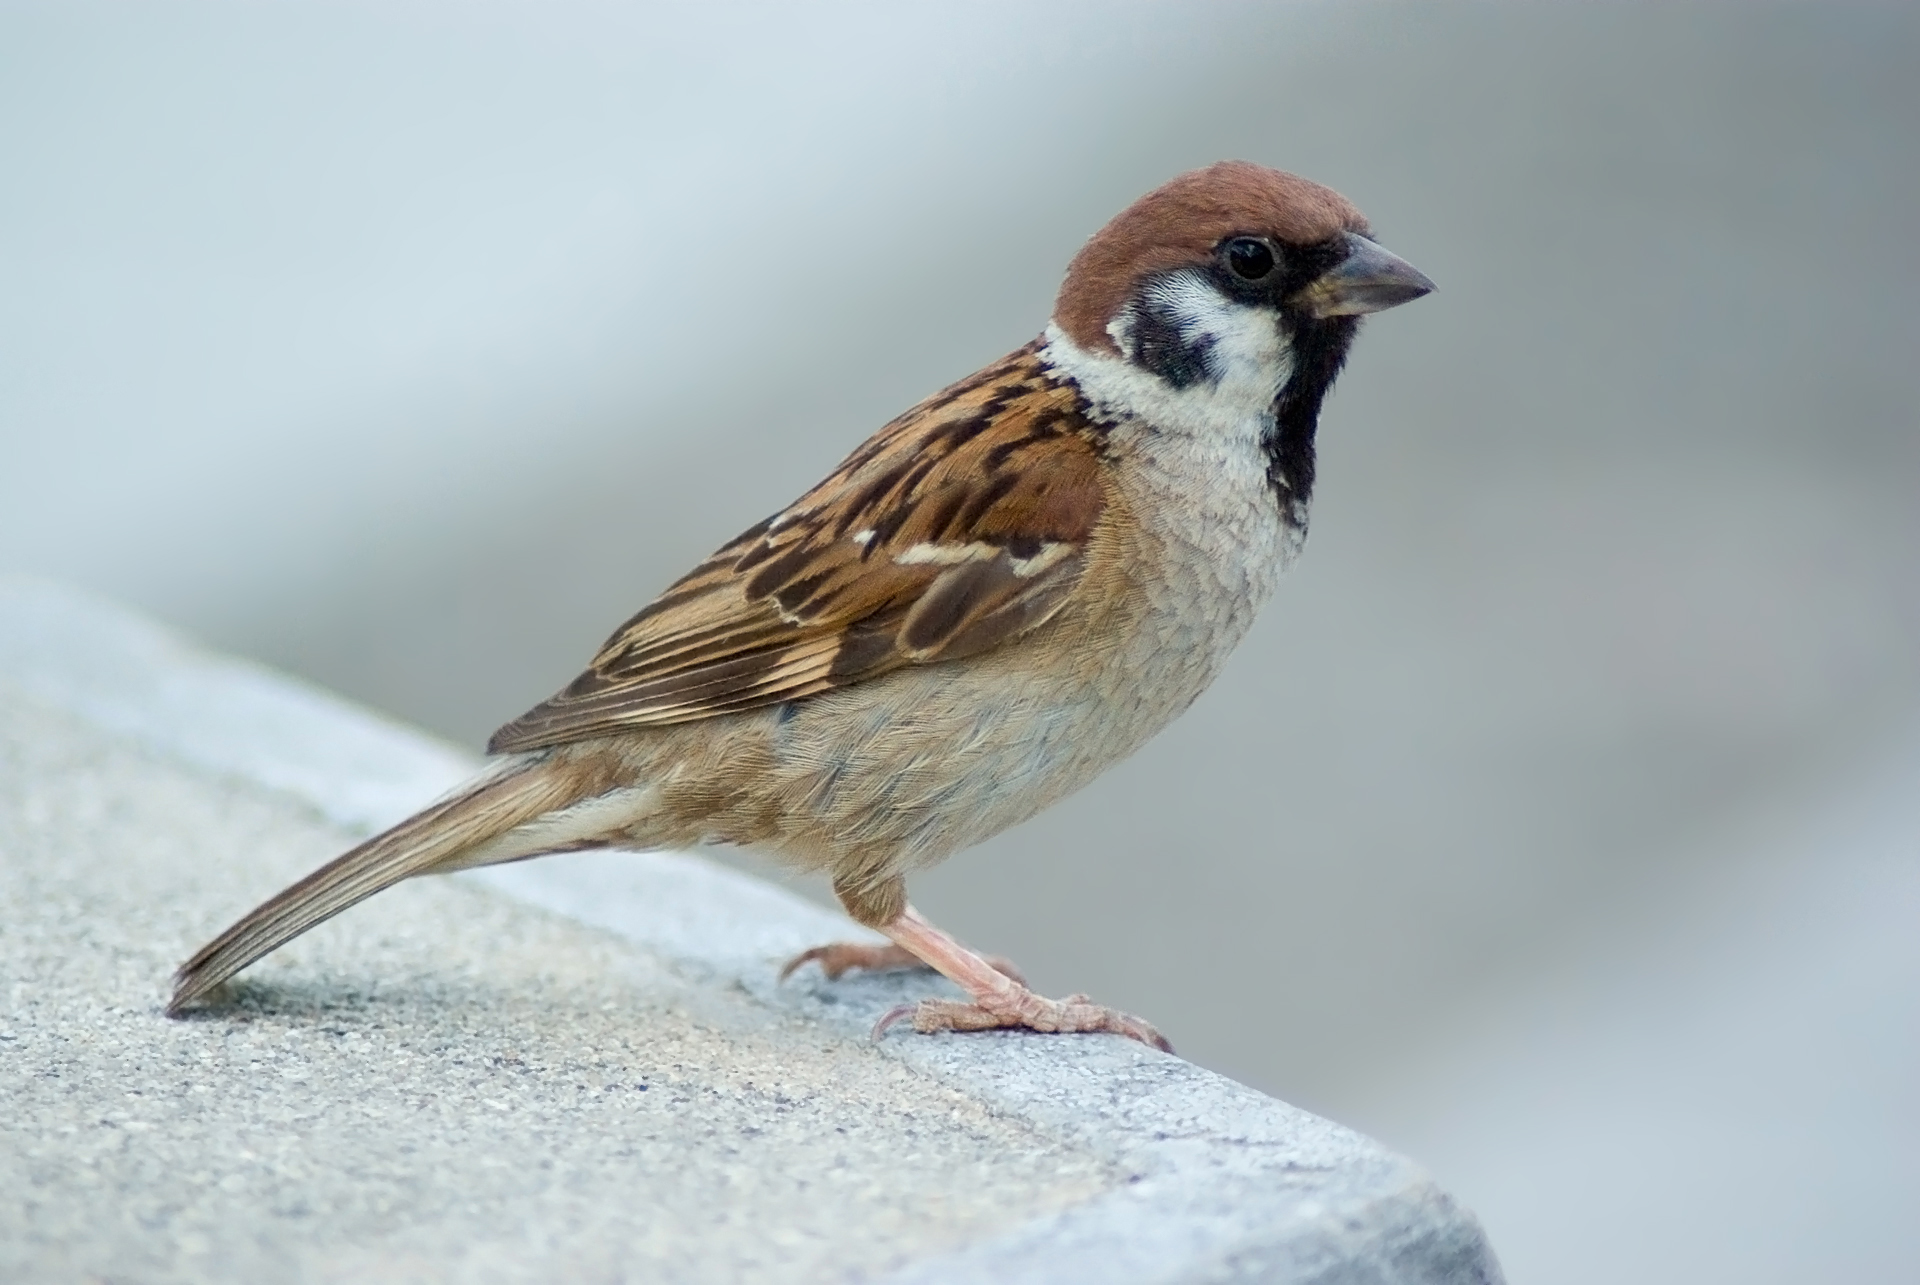
\includegraphics[width=0.4\textwidth]{\GRAPHPATH/spatz}}}$
    \onslide<+->
    \hspace*{0.025\textwidth}>\hspace*{0.025\textwidth}
    $\vcenter{\hbox{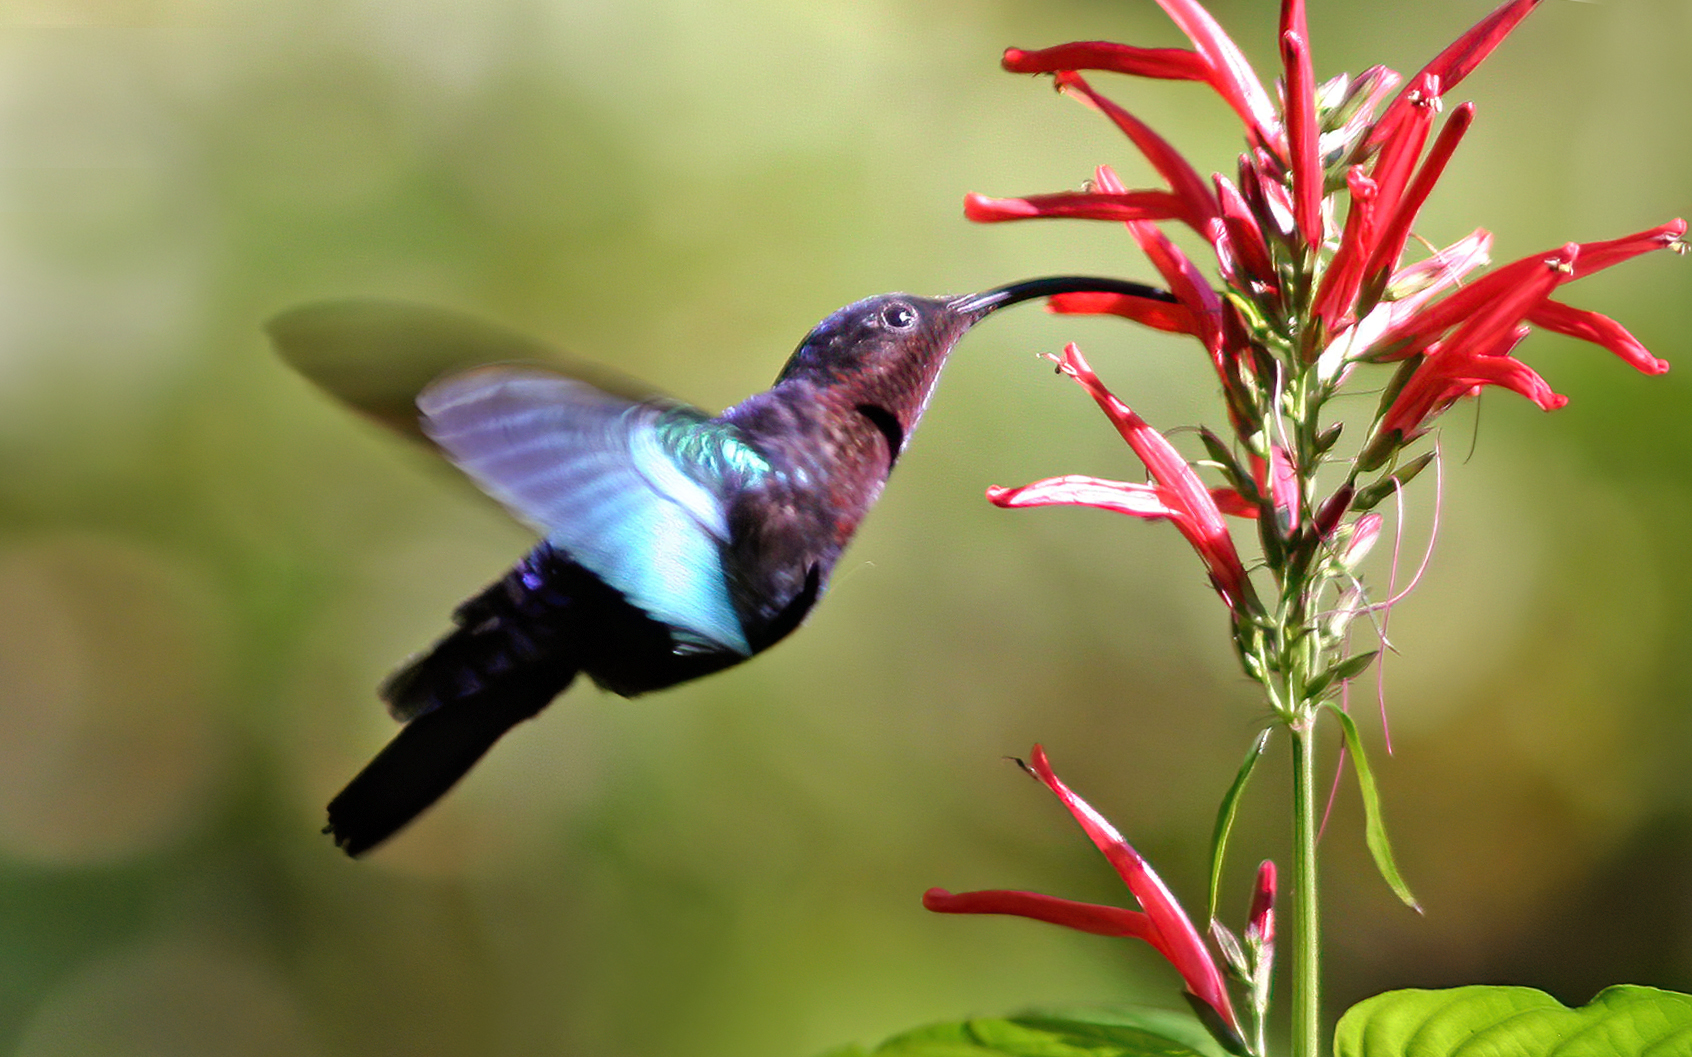
\includegraphics[width=0.25\textwidth]{\GRAPHPATH/kolibri}}}$
    \onslide<+->
    \hspace*{0.025\textwidth}>\hspace*{0.025\textwidth}
    $\vcenter{\hbox{\includegraphics[width=0.1\textwidth]{\GRAPHPATH/kiwi}}}$
  \end{minipage}\\
  \Halbzeile
  \centering 
  \grau{\tiny Bildquelle: Wikipedia}
\end{frame}

\begin{frame}
  {Programmatisches Schlussbild | Antwort}
  \onslide<+->
  \onslide<+->
  Die ewige Schwachsinnsfrage: Sind Kiwis und Pinguine nun \gruen{Vögel} oder nicht?\\
  \Viertelzeile
  \grau{Nur getoppt von: Erdbeeren sind gar keine Beeren, sondern Sammelnussfrüchte.}\\
  \Zeile
  \begin{itemize}[<+->]
    \item \alert{Kognition} | \orongsch{intrinsisch nicht diskret}, sondern ähnlichkeitsbasiert und \orongsch{parallel}
      \begin{itemize}[<+->]
        \item \orongsch{Netzwerkarchitektur}
      \end{itemize}
      \Halbzeile
    \item \alert{Symbole} = Phone, Morphe, Wörter, Phrasen, \ldots | \orongsch{intrinsisch} diskret und \orongsch{linear}
      \begin{itemize}[<+->]
        \item \orongsch{akustisches} Medium | Sagen Sie mal zwei Wörter gleichzeitig!
        \item \orongsch{schriftliches} Medium | Lesen Sie mal \textit{Zettels Traum} von Arno Schmidt\\
          \grau{(inkl.\ der Versuche, mehrere Wörter "`in einem"' zu schreiben)}
      \end{itemize}
    \Halbzeile
    \item[\ding{222}] Da wir nur akustisch oder über schriftliche Artefakte kommunizieren können,\\
      \alert{muss das Sprachsystem symbolisch sein}.
    \item[\ding{222}] Da es architekturbedingt nur nicht-symbolisch verarbeiten kann,\\
      \alert{muss das Gehirn symbolische Systeme so gut wie nötig und möglich emulieren}.
  \end{itemize}
\end{frame}


\begin{frame}
  {Programmatisches Schlussbild | Ausführung}
  \onslide<+->
  \onslide<+->
  Auch nicht-verschriftete Sprache muss medial bedingt logische Eigenschaften haben.\\
  \onslide<+->
  Kulturell bilden sich stärker symbolische Modi aus, vor allem durch Schrift.\\
  \grau{\footnotesize Norm, Selbst- und Fremdkorrektur, Textplanung, intensionale Definitionen, Explizierung, \ldots}\\
  \grau{\footnotesize Warum wird das vor allem im Kontext von Schule, Fremdsprache und Bildungssprache diskutiert?}\\
  \onslide<+->
  \Zeile
  \Halbzeile
  \centering 
  \begin{tabular}[h]{cc}
    \grau{(= spontane Sprachproduktion)} & \\
    \orongsch{weniger symbolische Eigenschaften} & \small \orongsch{informelle Alltagssprache} \\
    \onslide<+->
    \textcolor{orgrA}{\faArrowDown} &\large \textcolor{orgrA}{formelle Alltagssprache} \\
    \onslide<+->
    \textcolor{orgrB}{\faArrowDown} &\Large \textcolor{orgrB}{Bildungssprache} \\
    \onslide<+->
    \textcolor{orgrC}{\faArrowDown} &\LARGE \textcolor{orgrC}{Wissenschaftssprache} \\
    \onslide<+->
    \textcolor{orgrD}{\faArrowDown} &\huge \textcolor{orgrD}{Orthosprache} \\
    \onslide<+->
    \gruen{mehr symbolische Eigenschaften} & \gruen{\Huge formales System} \\
    \grau{(= reflektierte Sprachproduktion)}  & \\
  \end{tabular}
\end{frame}

\ifdefined\HANDOUT
  \begin{frame}
    {Und was ist denn nun mit Kiwis und Pinguinen?}
    \onslide<+->
    \onslide<+->
    Unser Verständnis der Welt führt zu genaueren und diskreten Kategorisierungen,\\
    \orongsch{wo dies nötig ist}. \alert{Die Sprache folgt dem erforderlichen Maß an Genauigkeit\slash Diskretheit.}\\
    \Zeile
    \onslide<+->
    \centering
    \begin{tikzpicture}
      \node at (0cm, 0cm) {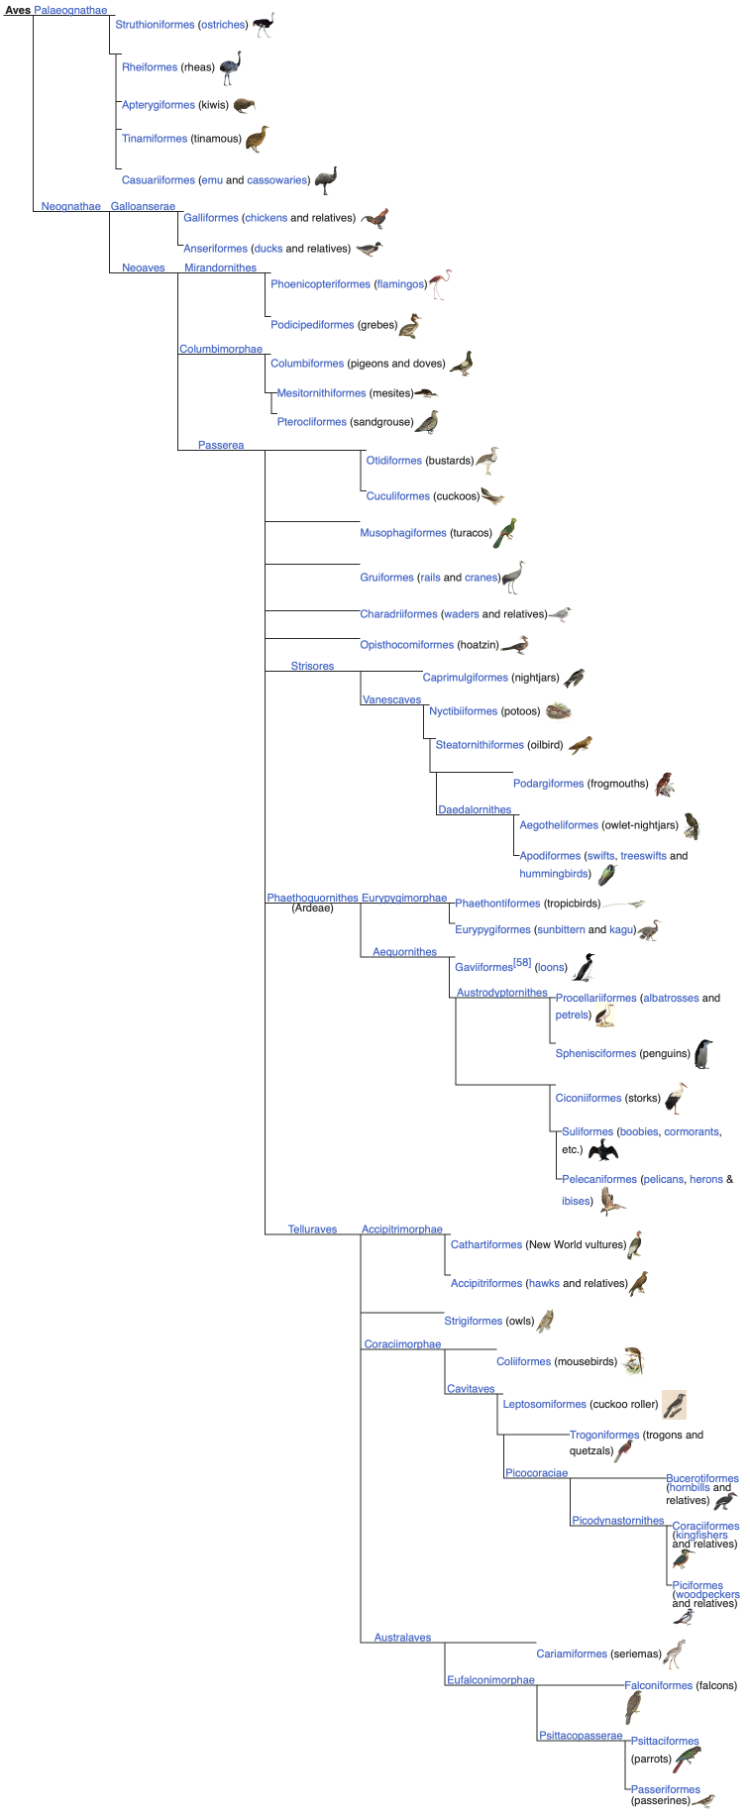
\includegraphics[height=0.6\textheight]{\GRAPHPATH/birds50}};
      \node at (5cm, 1.5cm) {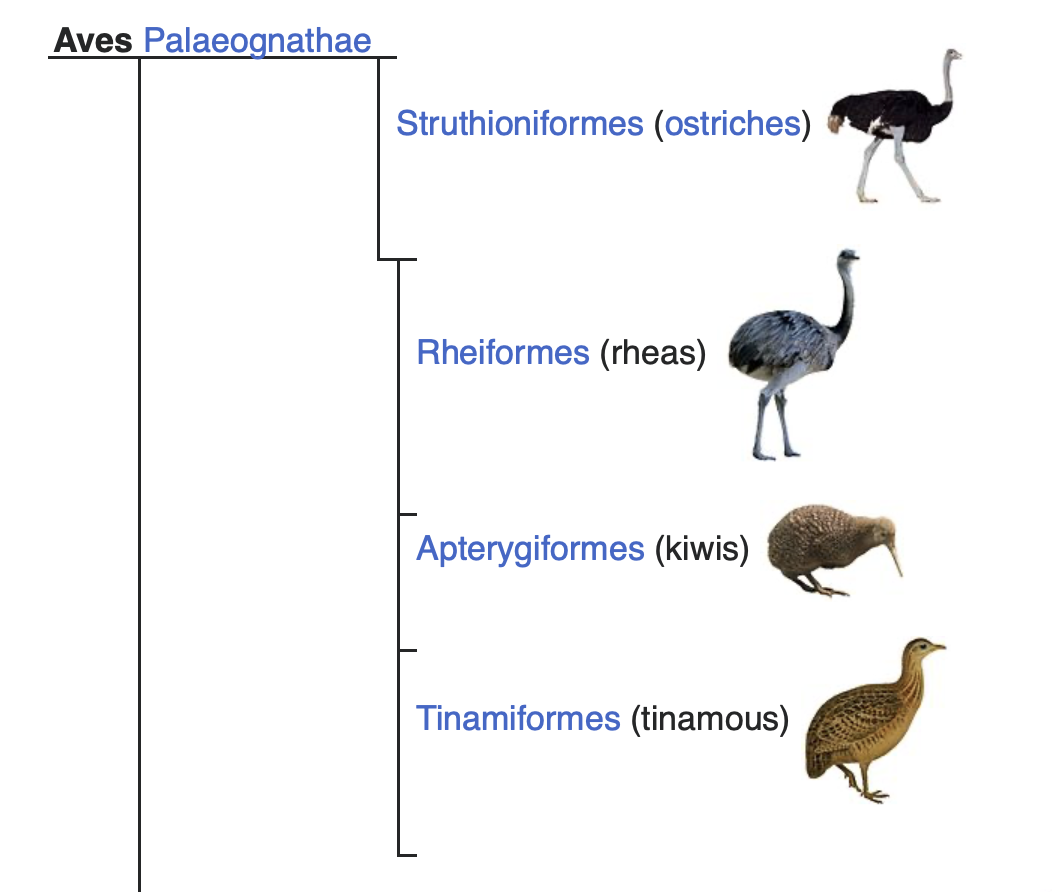
\includegraphics[height=0.25\textheight]{\GRAPHPATH/kiwis}};
      \node at (5cm, -1.5cm) {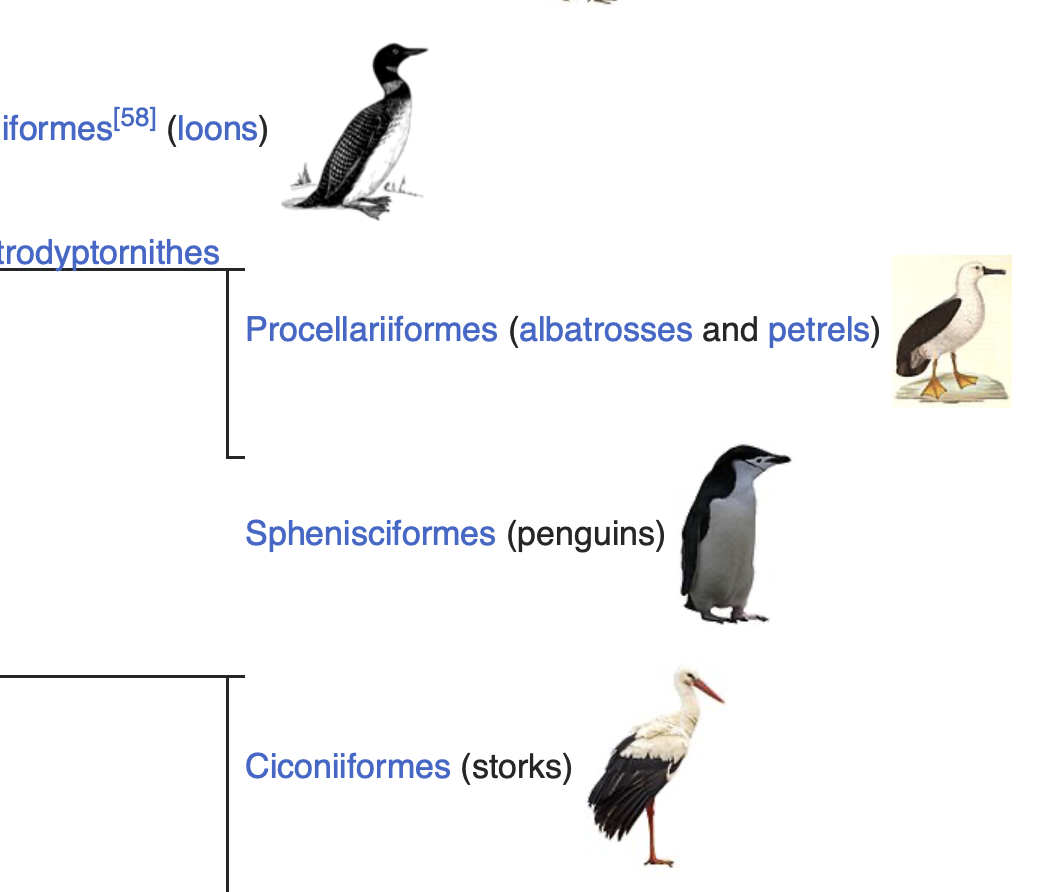
\includegraphics[height=0.25\textheight]{\GRAPHPATH/penguins}};
      \path (-0.3cm, 2.5cm) edge [-latex] (4.6cm, 1.25cm);
      \path (1.1cm, -0.45cm) edge [-latex] (4.2cm, -1.725cm);
    \end{tikzpicture}\\
    \Halbzeile
    \grau{\tiny Bildquelle: Wikipedia}
  \end{frame}
\else
  \begin{frame}
    {Und was ist denn nun mit Kiwis und Pinguinen?}
    \onslide<+->
    \onslide<+->
    Unser Verständnis der Welt führt zu genaueren und diskreten Kategorisierungen,\\
    wo dies nötig ist. \alert{Die Sprache folgt diesem Maß an Genauigkeit und Diskretheit!}\\
    \Zeile
    \onslide<+->
    \centering
    \begin{minipage}{0.9\textwidth}
    \centering
      $\vcenter{\hbox{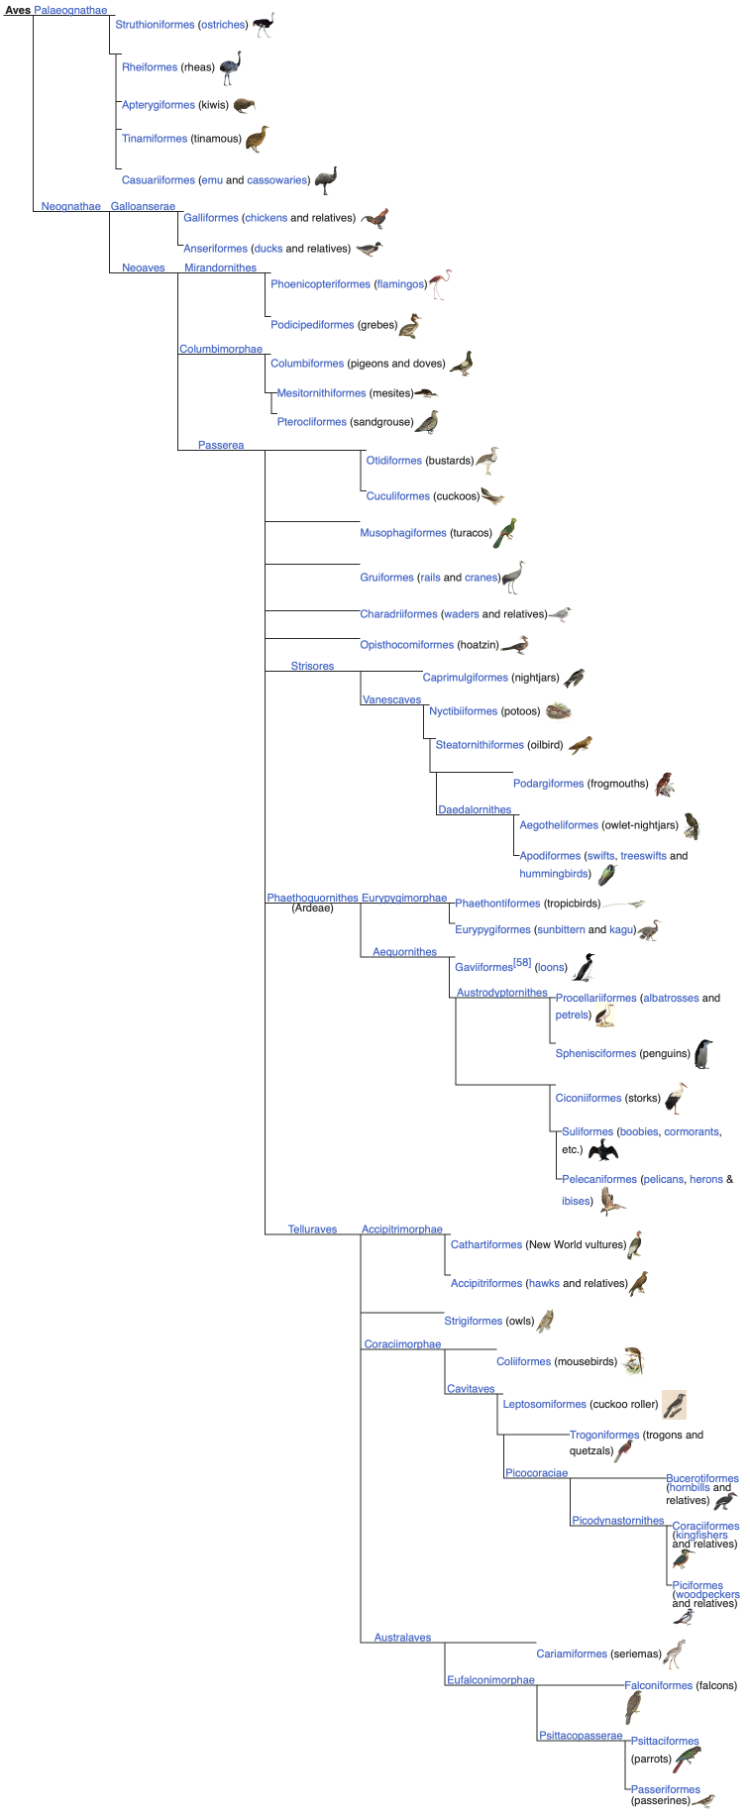
\includegraphics[height=0.7\textheight]{\GRAPHPATH/birds50}}}$\hspace{0.1\textwidth}
        \only<3>{$\vcenter{\hbox{\rule{0.4\textwidth}{0em}}}$}%
        \only<4>{$\vcenter{\hbox{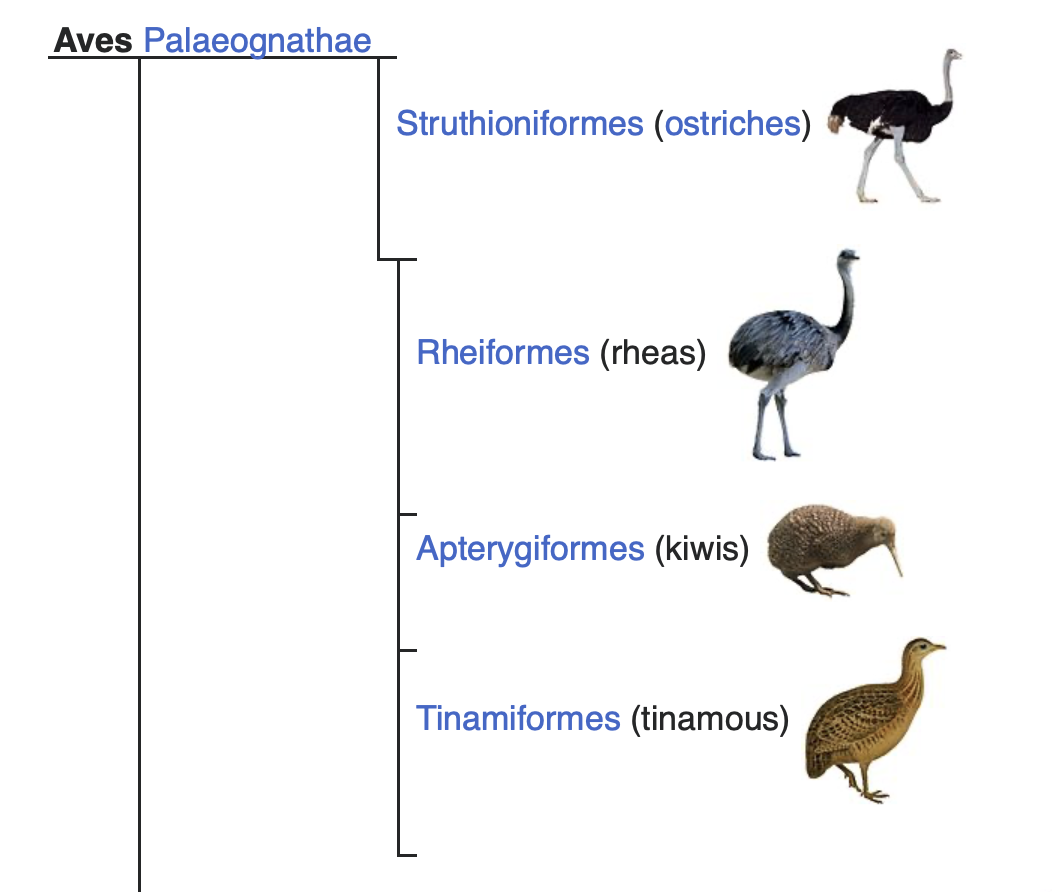
\includegraphics[width=0.4\textwidth]{\GRAPHPATH/kiwis}}}$}%
        \only<5>{$\vcenter{\hbox{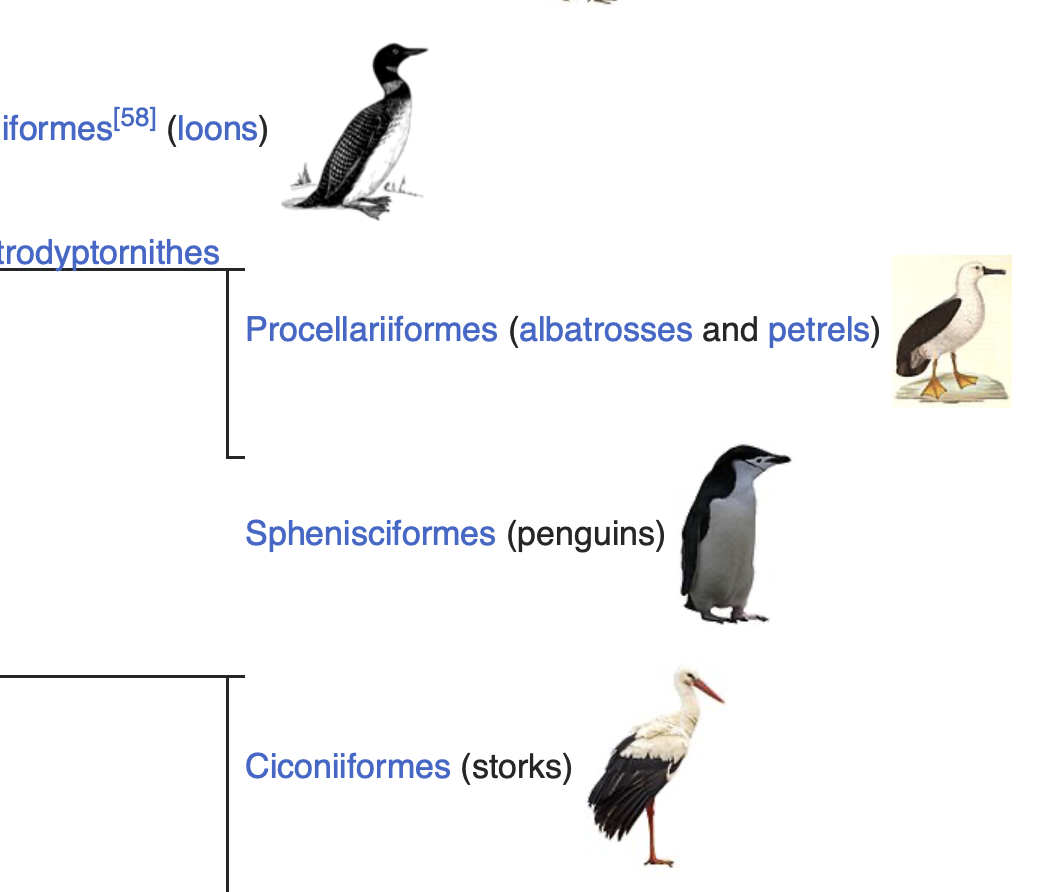
\includegraphics[width=0.4\textwidth]{\GRAPHPATH/penguins}}}$}
    \end{minipage}\\
    \grau{\tiny Bildquelle: Wikipedia}
  \end{frame}
\fi

\begin{frame}
  {Letzte Folie}
  \onslide<+->
  \begin{itemize}[<+->]
    \item Viele Missverständnisse in der Linguistik basieren darauf,\\
      dass das eben Gesagte nicht dem allgemeinen Forschungsprogramm zugrundeliegt.
    \item Die Doppelnatur von Sprache führt dazu, dass sowohl rein formale Linguistik\\
      und sogenannte kognitive Linguistik scheinbar erfolgreich sind.
    \item Im Prinzip läuft aber die Linguistik aktuell weitgehend ins Leere.
      \Halbzeile
    \item \alert{Modelltheoretische Semantik beschreibt einen essentiellen Teil von Sprache!}
    \item \alert{Sie modelliert logische Eigenschaften und den Bezug zur realen objektiven Welt.}
      \Halbzeile
    \item \small \grau{Ganz am Rande zu generativer AI:}
      \begin{itemize}[<+->]
        \item \grau{Erfolg | Sie modelliert völlig natürliche Grammatik.}
        \item \grau{Also alle traditionellen Grammatiker inkl.\ Chomsky: Setzen!}
        \item \grau{Gebrauchsbasiert ist generative AI sowieso. Also Stefan Gries: Setzen!}
          \Viertelzeile
        \item \grau{Misserfolg | Sie weiß nichts über die Welt im eigentlichne Sinn von \textit{Wissen}.}
        \item \grau{Wissen wird über die Verarbeitung eines immensen sprachlichen Inputs vorgetäuscht.}
        \item \grau{Es handelt sich um eine Art fancy Papagei.}
      \end{itemize}
  \end{itemize}
\end{frame}

  \let\subsection\section\let\section\woopsi

  \section[Referentielle Semantik]{Referentielle Semantik}
  \let\woopsi\section\let\section\subsection\let\subsection\subsubsection
  \section{Linguistische Theorien}

\begin{frame}
  {Ein neues semiotisches Dreieck}
  \onslide<+->
  \onslide<+->
  Im Sinn der letzten Woche interessiert uns nur die linke Seite.\\
  \onslide<+->
  \Zeile
  \centering 
  \begin{forest}
    [\gruen{Formen}
      [\gruen{Reale Objekte}, edge=gruen]
      [Mentale Konzepte]
    ]
  \end{forest}
\end{frame}

\begin{frame}
  {"`Semantik"' im generativen T-Modell}
  \onslide<+->
  \onslide<+->
  \centering 
  \resizebox{0.6\textwidth}{!}{
    \begin{tikzpicture}

      \node [rectangle, draw, align=left, color=teal, rounded corners=0.5em] (Numeration) at (5cm, -6cm) {Numeration};
      
      \node [visible on=<3->, rectangle, draw, align=left, color=gray] (Lexikon) at (1cm, -6cm) {Lexikon};
      \path (Lexikon.east) edge [visible on=<3->, line width=0.5mm, dashed] node [below, shift={(-0.4cm,0)}] {\textit{}} (Numeration.west);
     
      \node [visible on=<4->, rectangle, draw, align=left, color=gray] (Intention) at (9cm, -6cm) {Intention};
      \path (Intention.west) edge [visible on=<4->, line width=0.5mm, dashed] node [below, shift={(-0.4cm,0)}] {\textit{}} (Numeration.east);

      \node [visible on=<5->, rectangle, draw, align=left, fill=black, color=black, rounded corners=0.5em] (Syntax) at (5cm, -4.5cm) {\whyte{Syntax}};
      \path (Numeration.north) edge [visible on=<5->, line width=0.5mm, -latex] node [below, shift={(-0.4cm,0)}] {\textit{}} (Syntax.south);  

      \node [visible on=<6->, rectangle, draw, align=left, color=teal, rounded corners=0.5em] (Phrasenstruktur) at (5cm, -3cm) {Phrasenstruktur};
      \path (Syntax.north) edge [visible on=<6->, line width=0.5mm, -latex] node [below, shift={(-0.4cm,0)}] {\textit{}} (Phrasenstruktur.south);  

      \node [visible on=<7->, rectangle, draw, align=left, color=teal, rounded corners=0.5em] (PF) at (4cm, 0cm) {PF};
      \path (Phrasenstruktur.north) edge [visible on=<7->, line width=0.5mm, -latex] node [below, shift={(-0.4cm,0)}] {\textit{}} (PF.south);  
     
      \node [visible on=<8->, rectangle, draw, align=left, color=gray] (Aeusserung) at (1cm, 0cm) {Äußerung};
      \path (Aeusserung.east) edge [visible on=<8->, line width=0.5mm, dashed] node [below, shift={(-0.4cm,0)}] {\textit{}} (PF.west);
     
      \node [visible on=<9->, rectangle, draw, align=left, fill=black, color=black, rounded corners=0.5em] (Syntax2) at (6cm, -1.5cm) {\whyte{Syntax 2}};
      \path (Phrasenstruktur.north) edge [visible on=<9->, line width=0.5mm, -latex] node [below, shift={(-0.4cm,0)}] {\textit{}} (Syntax2.south);  
     
      \node [visible on=<10->, rectangle, draw, align=left, color=teal, rounded corners=0.5em] (LF) at (6cm, 0cm) {LF};
      \path (Syntax2.north) edge [visible on=<10->, line width=0.5mm, -latex] node [below, shift={(-0.4cm,0)}] {\textit{}} (LF.south);  

      \node [visible on=<11->, rectangle, draw, align=left, color=gray] (Interpretation) at (9cm, 0cm) {Interpretation};
      \path (Interpretation.west) edge [visible on=<11->, line width=0.5mm, dashed] node [below, shift={(-0.4cm,0)}] {\textit{}} (LF.east);
      
    \end{tikzpicture}
  }
\end{frame}

\begin{frame}
  {Repräsentationsebenen}
  \onslide<+->
  \onslide<+->
  Im klassischen generativen Modell:\\
  \grau{\footnotesize (In minimalistischen Modellen herrscht -- Chomsky muss es mögen! -- sowieso Anarchie.)}
  \Zeile
  \begin{itemize}[<+->]
    \item keine echte Interpretation auf LF
    \item Bewegung \rot{nachdem} der Satz geäußert wurde
    \item Herstellung einer logisch interpretierbaren \alert{Form} auf LF
    \item Grund | Syntax kann nicht alle Interpretationen abbilden
      \Halbzeile
      \begin{itemize}[<+->]
        \item[ ] \alert{Klassiker Quantorenskopus}
        \item[ ] \textit{Everybody loves somebody.}
          \Viertelzeile
        \item[A] Für alle Personen y gilt, dass es eine Person x gibt, für die gilt: y liebt x \grau{($\forall y\exists x.L(y,x)$)}
        \item[B] Es gibt eine Person x, sodass für alle Personen y gilt: y liebt x \grau{($\exists x\forall y.L(y,x)$)}
      \end{itemize}
  \end{itemize}
\end{frame}


\begin{frame}
  {Montagues direkte Interpretation}
  \onslide<+->
  \onslide<+->
  Sprache ist Logik ist Sprache \ldots\\
  \Halbzeile
  \begin{itemize}[<+->]
    \item[A] Entweder ist die \alert{Übersetzung in eine LF trivial und äquivalent zur PF\slash Syntax},\\
      oder \orongsch{sie fügt etwas hinzu, dass der Sprache an sich fehlt}.
    \item[B] Sätze haben aber auch \alert{mit LF-Übersetzung nur die Bedeutungen,\\
      die sie sowieso haben} \grau{(keine Hinzufügung)}.
    \item[\ding{222}] Also ist die \gruen{Übersetzung in LF trivial und äquivalent zur PF\slash Syntax}.
    \item[\ding{222}] Wir können \gruen{Sätze direkt interpretieren} (wie sie gesprochen\slash geschrieben werden).
     \Zeile 
   \item \alert{Montagues \textit{lf}} | direkte Übersetzung von sprachlichen in logische Ausdrücke
  \end{itemize}
\end{frame}

\section{Referentielle Semantik basal}

\begin{frame}
  {Interessante Eigenschaften von Sprache}
  \onslide<+->
  \begin{itemize}[<+->]
    \item Aussagen über die\slash Teile der Welt
    \item Ausdrücke bezeichnen\slash referieren auf Dinge i.\,w.\,S.
    \item Informativität
    \item objektiv beurteilbar (\zB Wahrheit von Sätzen)
      \Zeile
    \item \alert{Aber welche sprachlichen Einheiten referieren auf was?}
  \end{itemize}
\end{frame}

\begin{frame}
  {Referenz | Eigennamen}
  \onslide<+->
  \onslide<+->
  Ein \alert{Eigenname} \ding{222} \alert{genau ein Objekt} in der Welt\\
  \onslide<+->
  \Zeile
  \centering
    \begin{tikzpicture}
      \node [] (name) at (-6cm, 0cm) {\textit{Jan Böhmermann}};
      \node [visible on=<4->] (boehmi) at (0cm, 0cm) {\includegraphics[width=0.2\textwidth]{\GRAPHPATH/boehmermann}};
      \path (name.east) edge [visible on=<4->, line width=0.5mm, -latex] node {\textit{}} (boehmi.west);
    \end{tikzpicture}
\end{frame}

\begin{frame}
  {Referenz | Appellativa}
  \onslide<+->
  \onslide<+->
  Ein normales \alert{Nomen} \ding{222} \alert{eine Menge von Objekten} in der Welt\\
  \onslide<+->
  \Zeile
  \centering
    \begin{tikzpicture}
      \node [] (noun) at (-6cm, 0cm) {\textit{soldier}};
      \node [visible on=<4->] (soldiers) at (0cm, 0cm) {
\includegraphics[width=0.2\textwidth]{\GRAPHPATH/soldiers}};
      \path (noun.east) edge [visible on=<4->, line width=0.5mm, -latex] node {\textit{}} (soldiers.west);
    \end{tikzpicture}
\end{frame}

\begin{frame}
  {Referenz | Adjektive und Verben}
  \onslide<+->
  \onslide<+->
  Ein (intersektives) \alert{Adjektiv} oder ein \alert{Verb} \ding{222} \alert{eine Menge von Objekten} in der Welt\\
  \onslide<+->
  \Zeile
  \centering
    \begin{tikzpicture}
      \node [] (adj) at (-6cm, 0cm) {\textit{human}};
      \node [visible on=<4->] (boehmi) at (0cm, +2cm) {\includegraphics[width=0.1\textwidth]{\GRAPHPATH/boehmermann}};
      \path (adj.east) edge [visible on=<4->, line width=0.5mm, -latex] node {\textit{}} (boehmi.west);
      \node [visible on=<5->] (soldiers) at (0cm, 0cm) {
\includegraphics[width=0.1\textwidth]{\GRAPHPATH/soldiers}};
      \path (adj.east) edge [visible on=<5->, line width=0.5mm, -latex] node {\textit{}} (soldiers.west);
      \node [visible on=<6->] (crowd) at (0cm, -2cm) {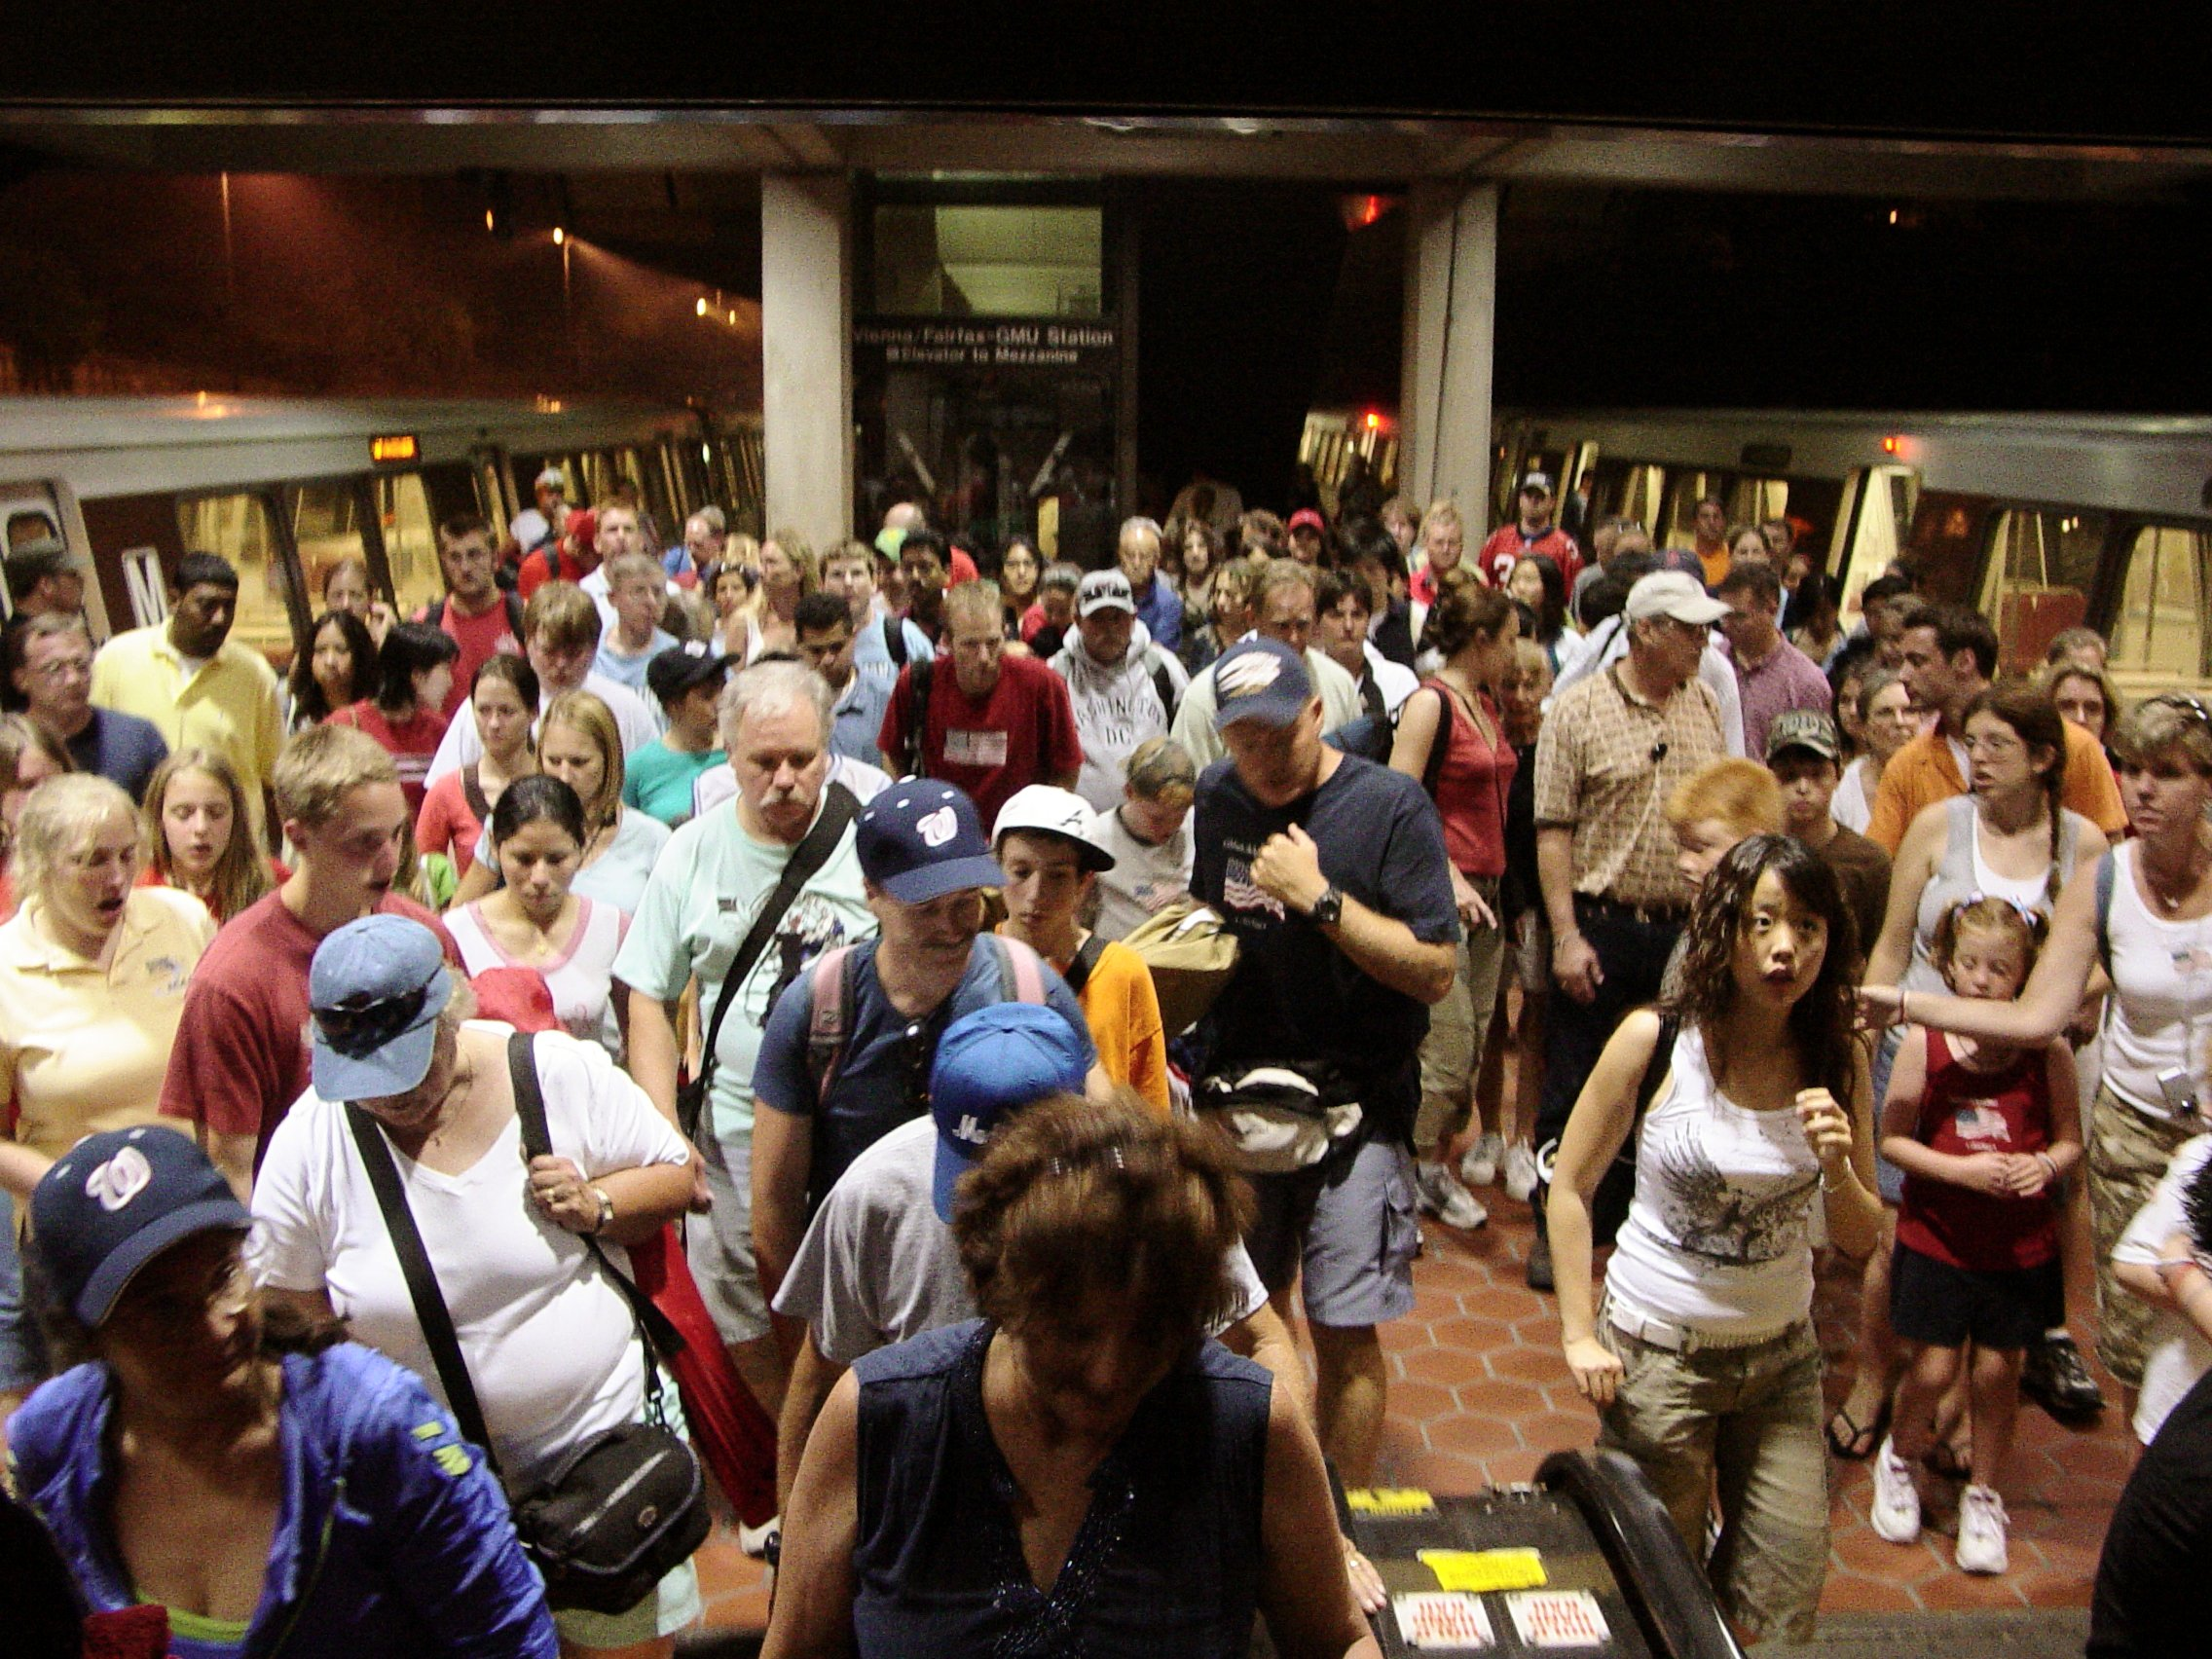
\includegraphics[width=0.1\textwidth]{\GRAPHPATH/crowd}};
      \path (adj.east) edge [visible on=<6->, line width=0.5mm, -latex] node {\textit{}} (crowd.west);
    \end{tikzpicture}
\end{frame}

\begin{frame}
  {Referenz | Sätze}
  \onslide<+->
  \onslide<+->
  Ein \alert{Satz} \ding{222} in erster Näherung \alert{ein Sachverhalt}\\
  \onslide<+->
  \Zeile
  \centering
    \begin{tikzpicture}
      \node [align=left] (s) at (-6cm, 0cm) {\it A humming bird\\\it is hovering over\\\it a red flower.};

      \node [visible on=<4->, align=center] (hum) at (0cm, +2cm) {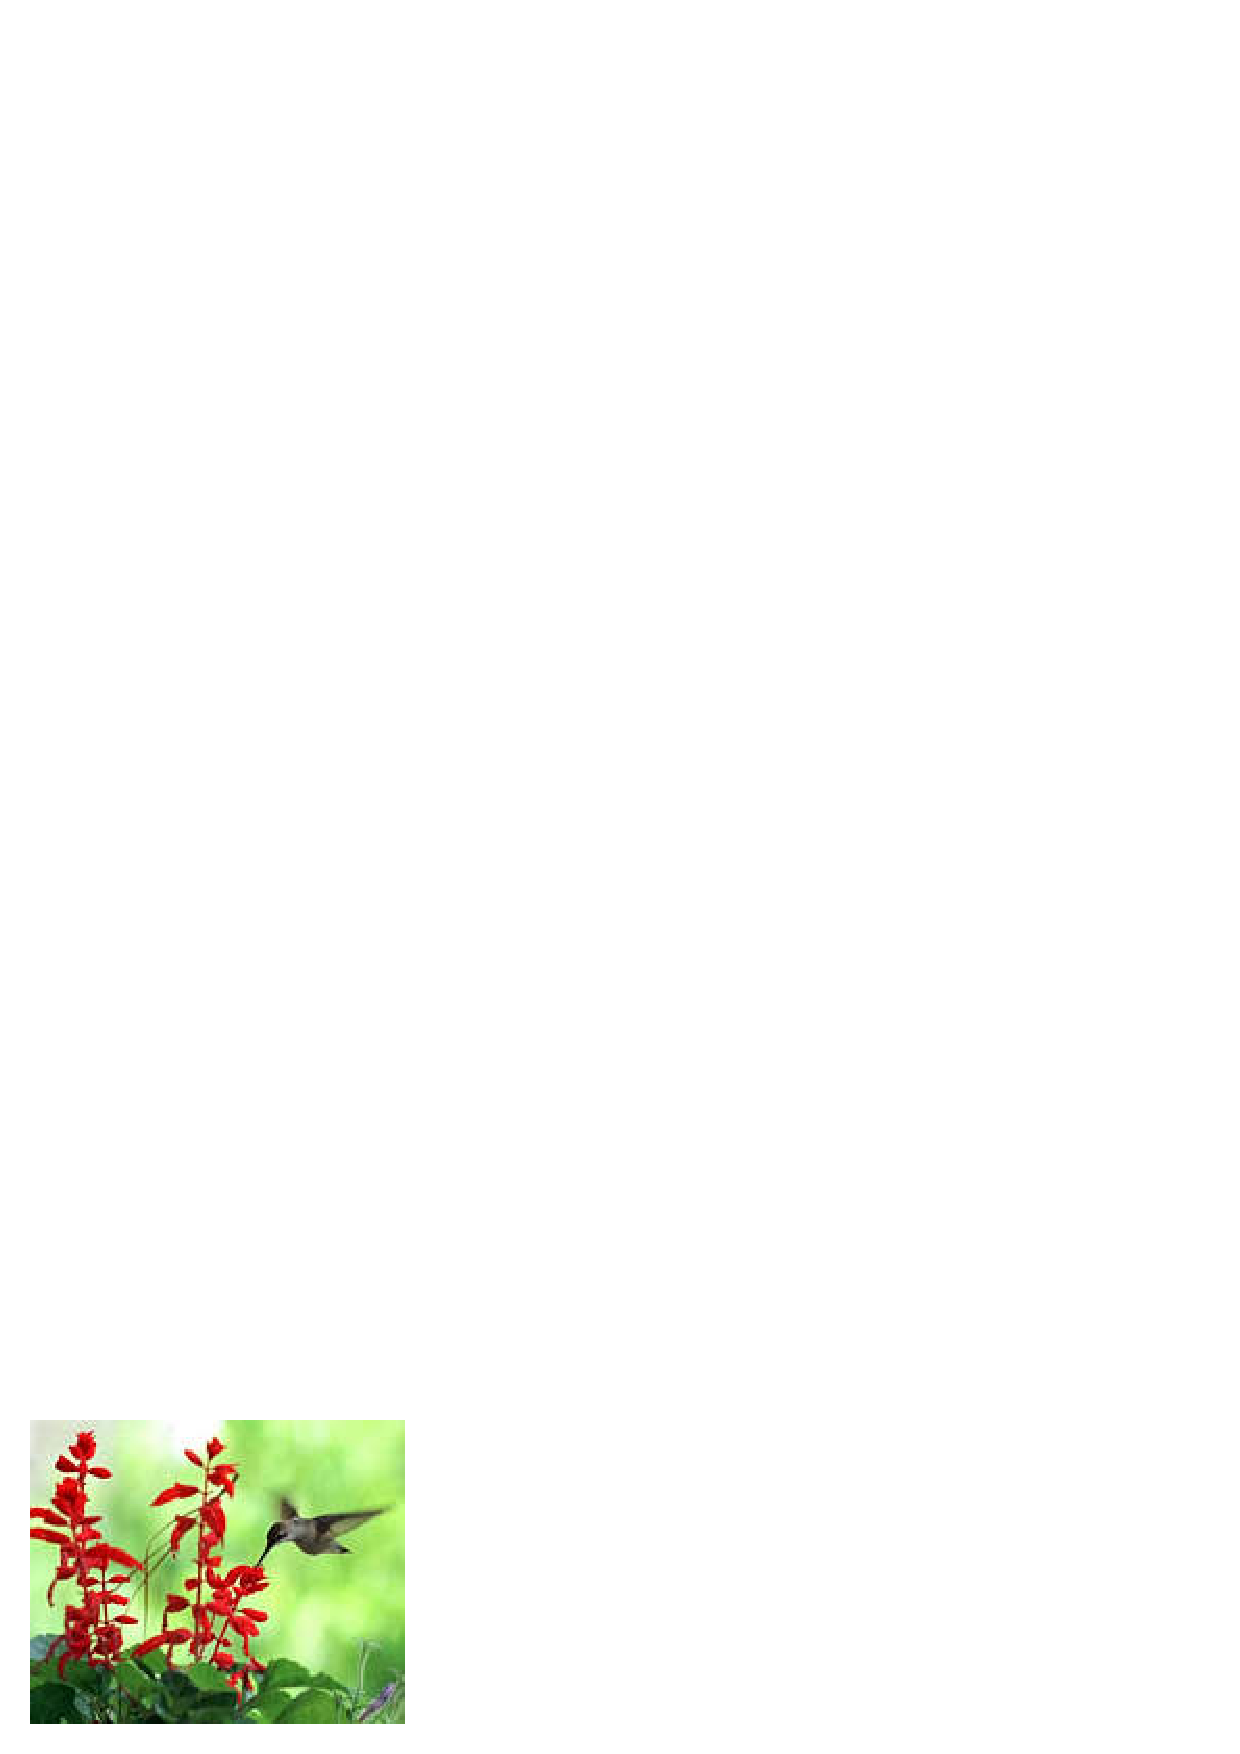
\includegraphics[width=0.2\textwidth]{\GRAPHPATH/hummingbird}};
      \path (s.east) edge [visible on=<4->, line width=0.5mm, -latex] node {\textit{}} (hum.west);
      
      \node [visible on=<5->, align=center] (boehmi) at (0cm, -2cm) {\includegraphics[width=0.2\textwidth]{\GRAPHPATH/boehmermann}\\\footnotesize (als Individuum)};
      \path (s.east) edge [visible on=<5->, line width=0.5mm, -latex, color=red] node {\textit{}} (boehmi.west);
      \node [visible on=<6->, align=center, color=red, fill=red] (nein) at (-3.5cm, -1.25cm) {\footnotesize \whyte{Nein! falsche}\\\footnotesize \whyte{Art von Objekt}};
    \end{tikzpicture}
\end{frame}

\begin{frame}
  {Freges Prinzip | Das hier wollen wir formalisieren!}
  \onslide<+->
  \onslide<+->
  Bedeutung ist kompositional!\\
  \Halbzeile
  \begin{itemize}[<+->]\small
    \item \textit{humming bird} \ding{222} die \alert{Menge} der Kolibri-Objekte
    \item \textit{a} \ding{222} \alert{Existenzaussage} für ein Element aus einer Menge
    \item \textit{a humming bird} \ding{222} \alert{Existenzaussage} für ein Element $x$\\
      aus der Menge der Kolibri-Objekte
    \item \textit{is hovering} \ding{222} die \alert{Menge} der schwebenden Objekten
    \item \textit{a humming bird is hovering} \ding{222} das existierende Kolibri-Objekt $x$\\
      ist auch ein \alert{Element der Menge} der schwebenden Objekte
    \item \textit{a red flower} \ding{222} \alert{Existenzaussage} für ein Element $y$\\
      aus der \alert{Schnittmenge} der roten Objekte und der Blumen-Objekte
    \item \textit{over} \ding{222} die \alert{Relation} zwischen Objekten (s.\ nächste Woche),\\
      die sich übereinander befinden
    \item \textit{A Humming is hovering over a red flower.} \ding{222}\\
      \gruen{Es gibt ein Objekt $x$ aus der Schnittmenge der Kolibri- und der schwebenden Objekte,\\
      und es gibt ein Objekt $y$ aus der Schnittmenge der roten und der Blumen-Objekte,\\
    und $x$ befindet sich über $y$.}
  \end{itemize}
\end{frame}

\section{Semantische Eigenschaften von Sätzen}

\begin{frame}
  {Implikation (Entailment)}
  \onslide<+->
  \onslide<+->
  Mengen von Aussagesätzen \alert{implizieren} andere Sätze.\\
  \onslide<+->
  Sätze (Implikationen) lassen sich aus anderen Sätzen (Axiome) \alert{beweisen}.\\
  \Halbzeile
  \begin{itemize}[<+->]
    \item[A] \textit{Jan Böhmermann ist ein Mensch.}
    \item[B] \textit{Jan Böhmermann ist leutselig.}
    \item[C] \textit{Jan Böhmermann ist ein leutseliger Mensch.}
      \Halbzeile
    \item[ ] \alert{$A,B\vdash C$} | A und B implizieren C. (C ist beweisbar aus A und B.)
    \item[ ] \rot{$A\not\vdash C$} | A impliziert nicht C.
    \item[ ] \rot{$B\not\vdash C$} | B impliziert nicht C.
      \Halbzeile
    \item[ ] \orongsch{$A\vdash A\wedge A$} \onslide<+->| \textit{Jan Böhmermann ist ein Mensch \orongsch{und} Jan Böhmermann ist ein Mensch.}
      \Halbzeile
    \item[D] \textit{Irgendetwas ist ein Mensch.}
    \item[ ] \alert{$A\vdash D$} 
  \end{itemize}
\end{frame}

\begin{frame}
  {Tests auf Implikation}
  \onslide<+->
  \onslide<+->
  Wenn diese Kriterien zutreffen, impliziert A B:\\
  \Zeile
  \begin{itemize}[<+->]
    \item Wenn A wahr ist, ist B auch immer wahr.
    \item Eine Situation, die von B beschrieben wird, wird auch von A beschrieben.
    \item Die Information in B ist vollständig in der Information in A enthalten.
    \item Man kann unter keinen Umständen sagen: \textit{A ist wahr, aber B ist nicht wahr.}
  \end{itemize}
\end{frame}

\begin{frame}
  {Übung | Sind das Implikationen?}
  \begin{itemize}[<+->]\small
    \item Böhmermann ist Showmaster. $\vdash$ Böhmermann ist menschlich.
    \item Böhmermann ist nicht sehr groß. $\vdash$ Irgendjemand ist nicht sehr groß.
    \item Böhmermann ist nicht sehr groß. $\vdash$ Irgendjemand ist sehr groß.
    \item Manche Menschen sind leutselig. $\vdash$ Böhmermann ist leutselig.
    \item Ich habe das neue drip-133-Album gehört. $\vdash$ drip-133 hat ein neues Album veröffentlicht.
    \item Nachdem ich einen Sherry getrunken habe, habe ich den Kondensator getauscht.\\
      $\vdash$ Ich habe einen Sherry getrunken.
    \item Nachdem Linux nicht mehr startete, habe ich einen weiteren Sherry getrunken.\\
      $\vdash$ Linux ist noch nie gestartet.
    \item Mein ehemaliger Mitbewohner mag Becks.\\
      $\vdash$ Mein ehemaliger Mitbewohner könnte Sherry mögen.
    \item Böhmermann hat das heutige ZDF Magazin beendet.\\
      $\vdash$ Das heutige ZDF Magazin wurde beendet.
  \end{itemize}
\end{frame}

\begin{frame}
  {Präsupposition | Der plausible HIntergrund}
  \onslide<+->
  \onslide<+->
  Präsuppositionen sind schwächer als Implikationen.\\
  \Zeile
  \begin{itemize}[<+->]
    \item[A] \textit{Willy Brandt ist der gegenwärtige Kanzler Deutschlands.}
    \item[B] \textit{Wenn Willy Brandt der gegenwärtige Kanzler Deutschlands ist,\\
      trägt er eine große Verantwortung.}
    \item[C] \textit{Willy Brandt ist nicht der gegenwärtige Kanzler Deutschlands.}
    \item[D] \textit{Willy Brandt lebt.}
    \item[E] \textit{Es gibt einen Kanzler Deutschlands.}
      \Halbzeile
    \item \alert{A und B präsupponieren D.} = D ist eine Voraussetzung\\
      für eine erfolgreiche Interpretation von A und B.
    \item \orongsch{C präsupponiert nicht D.}
    \item \alert{A, B und C präsupponieren E.}
      \Halbzeile
    \item Die einzige Implikation hier: $A\vdash E$
  \end{itemize}
\end{frame}

\begin{frame}
  {Tests auf Präsupposition}
  \onslide<+->
  \onslide<+->
  Die Unterschiede zur Implikation sind relevant.\\
  \Halbzeile
  \begin{itemize}[<+->]
    \item Nicht nur Aussagesätzen haben Präsuppositionen (Modale, Konditionale, \ldots)
    \item Negierte Sätze haben oft gleiche Präsuppositionen wie nicht-negierte.
    \item Präsuppositionen können negiert werden, und der Ausgangssatz bleibt wahr.\\
      \grau{(Geht nicht mit Implikationen.)}
      \begin{itemize}[<+->]
        \item[F] \textit{Willy Brandt ist nicht Kanzler Deutschlands.}
        \item[G] \textit{Es gibt einen Kanzler Deutschlands.}
        \item[ ] F präsupponiert G, bleibt aber wahr, wenn G falsch ist.
      \end{itemize}
  \end{itemize}
\end{frame}

\begin{frame}
  {Synonymie}
  \onslide<+->
  \onslide<+->
  Synonyme Ausdrücke haben \orongsch{exakt} \alert{die gleiche Referenz}.\\
  \Halbzeile
  \begin{itemize}[<+->]
    \item lexikalische Synonymie | \textit{humming bird} $\stackrel{lex}{\equiv}$ \textit{colibri}
      \Halbzeile
    \item kompositionale Synonymie
      \begin{itemize}[<+->]
        \item[ ] \textit{Mulder traf seine entführte Schwester, nachdem er\\
          in die geheime Militärbasis eingebrochen war.}
        \item[$\equiv$] \textit{Bevor er seine entführte Schwester traf, brach Mulder in die geheime Militärbasis ein.}
      \end{itemize}
    \Halbzeile
    \item \alert{$A\equiv B\ \text{gdw}\ A\vdash B\ \text{und}\ B\vdash A$} (gegenseitige Implikation)
    \item \grau{\textit{gdw} = \textit{genau dann wenn} | \textit{iff} = \textit{if and only if}}
  \end{itemize}
\end{frame}

\section{Referenz von Sätzen}

% \subsection{Referential and non-referential NPs}
% \frame{\frametitle{Noun-like expressions and complex NPs}
%  \begin{itemize}
%    \item<1-> I saw \textcolor{blue}{a man}.
%    \item<2-> I saw \textcolor{blue}{the green wobbly thing crawling near}.
%    \item<3-> I saw \textcolor{blue}{it}.
%  \end{itemize}
% }
% 
% \frame{\frametitle{Problems with referential NPs}
%  \begin{itemize}
%    \item<1-> \emph{\textcolor{blue}{The dark subatomic particles in the universe} have a total mass much larger than the visible subatomic particles.}
%    \item<2-> \emph{\textcolor{blue}{Problems with referential semantic theories} don't concern \textcolor{blue}{Rumpletweezer}.}
%    \item<3-> \textcolor{red}{and of course, vagueness (e.g., Sorites Paradox)}
%  \end{itemize}
% }
% 
% \frame{\frametitle{Problems with non-referential NPs}
%  \begin{itemize}
%    \item<1-> \emph{some guy}
% 	 \item<2-> \emph{not the faintest trace of blood}
% 	 \item<3-> \emph{any axiom of Zermelo-Fraenkel set theory}
%  \end{itemize}
% }

\begin{frame}
  {Natürliche Sprache und Implikation}
  \onslide<+->
  \onslide<+->
  Referentielle Semantik $\not=$ \alert{\textit{Zeigen auf Objekte durch Sprache}}.\\
  \Viertelzeile
  \onslide<+->
  Zusätzliche Logik für Fälle wie diesen (und viele andere):\\
  \Zeile
  \onslide<+->
  \begin{tabular}[h]{lll}
    & \alert{\textit{Die Lieblingsblume meines Kolibris}} & \textit{ist rot.} \\
    \visible<6->{\orongsch{$\vdash$}} & \visible<5->{\alert{\textit{Eine Blume}} & \textit{ist rot.}} \\
  \end{tabular}
\end{frame}

\begin{frame}
  {Sätze referieren aus Wahrheitswerte!}
  \onslide<+->
  \onslide<+->
  \centering 
  Um zu der gewünschten Logik zu kommen, zeigen wir jetzt,\\
  dass \alert{Sätze auf Wahrheitswerte referieren}.\\
  \Halbzeile
  \onslide<+->
  Wahrheitswerte sind nur \alert{\textit{wahr}} und \alert{\textit{falsch}}.\\
  \Halbzeile
  \onslide<+->
  Die Verben \alert{\textit{denotieren}} und \textit{\alert{referieren auf}} sind hier synonym.\\
  \Doppelzeile
  \onslide<+->
  Warten Sie bitte ein paar Wochen, wenn Sie diese Darstellung reduktionistisch finden.
\end{frame}

\begin{frame}
  {Synonyme NPs}
  \onslide<+->
  \begin{itemize}[<+->]
    \item[a] \textit{colibri}
    \item[b] \textit{humming bird}
    \item[ ] \gruen{$a\stackrel{lex}{\equiv} b$}
      \Halbzeile
    \item[c] \textit{a brunette lady}
    \item[d] \textit{a brown-haired dame}
    \item[ ] \gruen{$c\equiv d$}
      \Halbzeile
    \item[e] \textit{the primates}
    \item[f] \textit{the apes and humans}
    \item[ ] \gruen{$e\equiv f$}
  \end{itemize}
\end{frame}

\begin{frame}
  {Synonymie von Konstituenten und Sätzen}
  Synonymie von Konstituenten im Satzkontext \ding{222} Satzsynonymie\\
  \onslide<+->
  \Halbzeile
  \begin{itemize}[<+->]
    \item[A] \alert{\textit{A \orongsch{colibri} is hovering over a red flower.}}
    \item[B] \alert{\textit{A \orongsch{humming bird} is hovering over a red flower.}}
    \item[ ] \gruen{$A\equiv B$ weil $a\equiv b$ und Satzkontext identisch}
      \Halbzeile
    \item[C] \alert{\textit{Lauren Bacall was \orongsch{a brunette lady}.}}
    \item[D] \alert{\textit{Lauren Bacall was \orongsch{a brown-haired dame}.}}
    \item[ ] \gruen{$C\equiv D$ weil $c\equiv d$ und Satzkontext identisch}
      \Halbzeile
    \item[E] \alert{\textit{\orongsch{Primates} are intelligent.}}
    \item[F] \alert{\textit{\orongsch{The apes and humans} are intelligent.}}
    \item[ ] \gruen{$E\equiv F$ weil $e\equiv f$ und Satzkontext identisch}
  \end{itemize}
\end{frame}

\begin{frame}
  {Zwei Axiome}
  \onslide<+->
  \begin{itemize}[<+->]
    \item[ ] Referenz\slash Denotat eines Ausdrucks A: \alert{\den{A}}
      \Zeile
    \item[ ] Erinnerung: Synonymität für Sätze ist gegenseitige Implikation.
      \Zeile
    \item[Ax1] Synonyme Ausdrücke (NPs, Verben, Sätze, \ldots) haben dieselbe Referenz.
    \item[ ] Formal: \alert{$A\equiv B\leftrightarrow\den{A}=\den{B}$}
      \Zeile
    \item[Ax2] Wenn wir in Ausdruck C einen Ausdruck A durch\\
      einen synonymen Ausdruck B ersetzen, behält C seine Referenz.
    \item[ ] Formal: \alert{$\den{A}=\den{B}\rightarrow\den{[\Sub{C} A]}=\den{[\Sub{C} B]}$}
  \end{itemize}
\end{frame}

\begin{frame}
  {Zwei wahre Sätze}
  \onslide<+->
  \onslide<+->
  Wahrheitswert von A und B | 1 bzw.\ \textit{wahr}\\
  \onslide<+->
  \Zeile
  \begin{itemize}[<+->]
    \item[A] \textit{Lauren Bacall was a brunette lady.}
    \item[B] \textit{My humming bird's favourite flower is red.} 
  \end{itemize}
\end{frame}

\begin{frame}
  {Erste Schlussfolgerung}
  \onslide<+->
  \onslide<+->
  Einsetzen von A und B in Satz T (Aussage über Wahrheitswert)\\
  \Halbzeile
  \begin{itemize}[<+->]
    \item[T] \alert{\textit{The truth value of `\_\_\_' is 1.}}
      \Halbzeile
    \item[{[\Sub{T}A]}] \alert{\textit{The truth value of `\orongsch{Lauren Bacall was a brunette lady.}' is 1.}}
    \item[{[\Sub{T}B]}] \alert{\textit{The truth value of `\orongsch{My humming bird's favourite flower is red.}' is 1.}}
      \Halbzeile
    \item[ ] folgt \gruen{$A\equiv[\Sub{T}A]$} und \gruen{$B\equiv[\Sub{T}B]$}
    \item[ ] mit Ax1 \gruen{$\den{A}=\den{[\Sub{T}A]}$} und \gruen{$\den{B}=\den{[\Sub{T}B]}$}
      \Halbzeile
    \item[ ] Bitte bedenken: $A$ und $[\Sub{T}A]$ haben auch intuitiv "`dieselbe Aussage"'.
  \end{itemize}
\end{frame}

\begin{frame}
  {Zweite Schlussforlgerung}
  \onslide<+->
  \onslide<+->
  In $[\Sub{T}A]$ und $[\Sub{T}B]$ sind A und B jeweils in einer NP eingebettet.\\
  \Halbzeile
  \begin{itemize}[<+->]
    \item $\den{the truth value of A}=\den{the truth value of B}=1$
    \item[ ] mit Ax2 \gruen{$\den{[\Sub{T}A]}=\den{[\Sub{T}B]}$}
    \item[ ] damit \gruen{$\den{A}=\den{[\Sub{T}A]}=\den{[\Sub{T}B]}=\den{B}=1$}
      \Halbzeile
    \item \gruen{Sätze referieren auf Wahrheitswerte.}\\
      \grau{(Denn man kann das mit zwei beliebigen wahren Sätzen machen.)}
  \end{itemize}
\end{frame}

\frame{\frametitle{Advantages of truth values}
\begin{itemize}
  \item<1-> indirect encoding of `richer' semantics (One must know the truth conditions of a sentence and the state of affairs to decide about the truth of a sentence.)
  \item<2-> a minimal common semantic property of sentences
  \item<3-> easily computable in a formal system (binary)
  \item<4-> their logic provides a basis for `richer' semantics (cf. second half of class)
\end{itemize}
}

\subsection{Sense and reference}
\frame{\frametitle{Frege also thought, reference couldn't be all}
\begin{center}
\begin{tabular}{|l|l|l|}
  \hline
  \textbf{Type} & \textbf{Reference} & \textbf{Sense} \\
  \hline
  \hline
  NP & individuals & individual concepts \\
      & \emph{Venus} & \\
  \hline
  VP & sets & property concepts \\
  & \emph{humming birds} & \\
  \hline
  S & 1 or 0 & thoughts \\
  & \emph{I like cats.} & \\
  \hline
\end{tabular}
\end{center}
}

\frame{\frametitle{Some terminology}
\begin{itemize}
  \item<1-> \emph{reference} = \emph{extension}	= what we're dealing with first
  \item<2-> \emph{sense} = \emph{intension} = what we will be dealing with later
  \item<3-> \emph{proposition} = the intensions of sentences as informational content: The `thought that S'.
\end{itemize}
}

\section{We're talking in fragments: F1}
\frame{\frametitle{Decomposing compositionality and composing truth}
\begin{itemize}
 \item<1-> How are sentences compositionally built up? 
 \item<2-> What do their parts denote?
 \item<3-> How does the denotation of the parts contribute to the whole.
 \item<4-> T-sentences: \textcolor{blue}{S of L is true in v iff p.}
 \item<5-> {\footnotesize \emph{S} a sentence, \emph{L} a language, \emph{v} a state of affairs, \emph{p} a statement of the truth conditions.}
\end{itemize}
}

\subsection{A syntax}

\frame{\frametitle{A phrase-structure grammar}
\begin{itemize}
 \item<1-> S $\rightarrow$ N VP
 \item<2-> S $\rightarrow$ S conj S	
 \item<3-> S $\rightarrow$	neg S
 \item<4-> VP $\rightarrow$ V\Sub{{i}}
 \item<5-> VP $\rightarrow$ V\Sub{t} N
\end{itemize}
}

\frame{\frametitle{A lexicon}
\begin{itemize}
 \item<1-> N $\rightarrow$ \emph{Herr Webelhuth, Frau Eckardt, the Turm-Mensa}
 \item<1-> V\Sub{{i}} $\rightarrow$ \emph{is relaxed, is creative, is stupid}
 \item<1-> V\Sub{t} $\rightarrow$ \emph{prefers}
 \item<1-> conj $\rightarrow$ \emph{and, or}
 \item<1-> neg $\rightarrow$ \emph{it is not the case that}
\end{itemize}
}

\subsection{The semantics: individuals, sets, functions, T-sentences}
\frame{\frametitle{Simple denotiations}
\begin{itemize}
  \item<1-> $\llbracket$Herr Webelhuth$\rrbracket$ = Herr Webelhuth
  \item<2-> $\llbracket$Frau Eckardt$\rrbracket$ = Frau Eckardt
  \item<3-> $\llbracket$the Turm-Mensa$\rrbracket$ = the Turm-Mensa
  \item<4-> $\llbracket$is relaxed$\rrbracket$ = \{x:x is relaxed\}
  \item<5-> $\llbracket$is creative$\rrbracket$ = \{x:x is creative\}
  \item<6-> $\llbracket$is stupid$\rrbracket$ = \{x:x is stupid\}
  \item<7-> $\llbracket$prefers$\rrbracket$ = \{$\langle$x,y$\rangle$: x prefers y\}
\end{itemize}
}

\frame{\frametitle{Some words don't really `denote', they act like functions}
\begin{itemize}
  \item<1-> $\dem{neg} = \left[
                         \begin{array}{l}
	                          1 \rightarrow 0\\
	                          0 \rightarrow 1
                         \end{array}
                         \right]$
  \item<2-> $\dem{and} = \left[
                         \begin{array}{l}
	                          \langle 1,1 \rangle \rightarrow 1\\
	                          \langle 1,0 \rangle \rightarrow 0\\
	                          \langle 0,1 \rangle \rightarrow 0\\
	                          \langle 0,0 \rangle \rightarrow 0
                         \end{array}
                         \right]$
  \item<3-> $\dem{or} = \left[
                         \begin{array}{l}
	                          \langle 1,1 \rangle \rightarrow 1\\
	                          \langle 1,0 \rangle \rightarrow 1\\
	                          \langle 0,1 \rangle \rightarrow 1\\
	                          \langle 0,0 \rangle \rightarrow 0
                         \end{array}
                         \right]$
  \end{itemize}
}

\frame{\frametitle{T-sentences: rule-to-rule}
\begin{itemize}
  \item<1-> \den{[\Sub{S}{ }N{ }VP]} = 1 iff \den{N} $\in$ \den{VP}, else 0
  \item<2-> \den{[\Sub{S} S1 conj S2]} = \den{conj} ($\langle$\den{S1},\den{S2}$\rangle$)
  \item<3-> \den{[\Sub{S} neg S]} = \den{neg} (\den{S})
  \item<4-> \den{[\Sub{VP} V\Sub{t} N]} = \{x: $\langle$x, \den{N} $\rangle$ $\in$ \den{V\Sub{t}}\}
  \item<5-> semantics for non-branching nodes: \textcolor{blue}{pass-up}
\end{itemize}
}

\subsection{Bottom-up evaluation}
\frame{\frametitle{A starting point for our computation}
\textcolor{blue}{\emph{Herr Webelhuth is relaxed.}}\\

\begin{itemize}
  \item<1-> Circumstances (Model): Herr Webelhuth is an element of the set of relaxed individuals.\\{}
  \item<2-> (1) The syntax is well-formed by S $\rightarrow$ N VP
  \item<3-> (2) for N: \den{Herr Webelhuth} = Herr Webelhuth
  \item<4-> (3) for VP: \den{is relaxed} = \{x: x is relaxed\}
  \item<5-> (4) for S: \den{[\Sub{S}{ }N{ }VP]} = 1 iff \den{N} $\in$ \den{VP}, else 0
\end{itemize}
}

\frame{\frametitle{A starting point for our computation}
The tree:\\

\begin{center}
 \begin{bundle}
   {1 since \den{Herr Webelhuth} $\in$ \den{is relaxed}}
     \chunk[N]{\den{Herr Webelhuth}}
     \chunk[VP]{\den{is relaxed}}
 \end{bundle}
\end{center}
}

\frame{\frametitle{We compute syntactic representations, not flat sentences}
\emph{\textcolor{blue}{(\Sub{S1} Frau Eckardt is creative)} and it is not the case that \textcolor{green}{(\Sub{S2} Herr Webehlhuth is relaxed)} and \textcolor{red}{(\Sub{S3} Frau Eckardt prefers the Turm-Mensa)}.}\\
\begin{center}
\begin{tabular}{cc}
 \begin{bundle}
   {S}\setlength\GapDepth{2ex}\setlength\GapWidth{1em}
   \chunk{\textcolor{blue}{S\Sub{1}}}
     \chunk{conj}
     \chunk{
             \begin{bundle}
               {S}
               \chunk{neg}
               \chunk{\begin{bundle}
                         {S}
                         \chunk{\textcolor{green}{S\Sub{2}}}
                         \chunk{conj}
                         \chunk{\textcolor{red}{S\Sub{3}}}
                       \end{bundle}
                     }
             \end{bundle}        
           }
 \end{bundle} &
 \begin{bundle}
   {S}\setlength\GapDepth{2ex}\setlength\GapWidth{1em}
     \chunk{\textcolor{blue}{S\Sub{1}}}
     \chunk{conj}
     \chunk{
             \begin{bundle}
               {S}
               \chunk{\begin{bundle}
                       {S}
                       \chunk{neg}
                       \chunk{\textcolor{green}{S\Sub{2}}}
                      \end{bundle}
                     }
               \chunk{conj}
               \chunk{\textcolor{red}{S\Sub{3}}}
             \end{bundle}        
           }
 \end{bundle}  \\
\end{tabular}
\end{center}
}

\frame{\frametitle{A starting point for our computation}
Circumstances: Herr Webelhuth is relaxed, Frau Eckardt is creative, and Frau Eckardt does not prefer the Turm-Mensa:\\

\begin{center}
\begin{tabular}{cc}
 \begin{bundle}
   {1}\setlength\GapDepth{2ex}\setlength\GapWidth{1em}
     \chunk{\textcolor{blue}{1}}
     \chunk{conj}
     \chunk{
             \begin{bundle}
               {1}
               \chunk{neg}
               \chunk{\begin{bundle}
                         {0}
                         \chunk{\textcolor{green}{1}}
                         \chunk{conj}
                         \chunk{\textcolor{red}{0}}
                       \end{bundle}
                     }
             \end{bundle}        
           }
 \end{bundle} &
 \begin{bundle}
   {0}\setlength\GapDepth{2ex}\setlength\GapWidth{1em}
     \chunk{\textcolor{blue}{1}}
     \chunk{conj}
     \chunk{
             \begin{bundle}
               {0}
               \chunk{\begin{bundle}
                       {0}
                       \chunk{neg}
                       \chunk{\textcolor{green}{1}}
                      \end{bundle}
                     }
               \chunk{conj}
               \chunk{\textcolor{red}{0}}
             \end{bundle}        
           }
 \end{bundle}  \\
\end{tabular}
\end{center}
}


  \let\subsection\section\let\section\woopsi

  \section[Mengen und Funktionen]{Mengen und Funktionen}
  \let\woopsi\section\let\section\subsection\let\subsection\subsubsection
  \begin{frame}
  {Kernfragen in dieser Woche}
  \onslide<+->
  \onslide<+->
  \centering 
  \Large
  Was sind \alert{Mengen}?\\
  \Halbzeile
  \onslide<+->
  Welche Operationen kann man auf Mengen anwenden?\\
  \onslide<+->
  \Halbzeile
  Was sind \alert{Relationen} und \alert{Funktionen}?\\
  Und wie hängen sie mit Mengen zusammen?\\
  \onslide<+->
  \Halbzeile
  Welche Eigenschaften können Funktionen und Relationen haben?
\end{frame}

\section{Mengen und Funktionen}

\begin{frame}
  {Was ist eine Menge?}
  \onslide<+->
  \onslide<+->
  Eine \alert{frei definierbare ungeordnete Sammlung von diskreten Objekten}\\
  \begin{itemize}[<+->]
    \item Zahlen
    \item Menschen
    \item Schuhe
    \item Wörter
    \item \ldots
      \Halbzeile
    \item nicht unbedingt zweckgebunden
    \item \orongsch{jedes Objekt maximal einmal in jeder Menge}
  \end{itemize}
  \centering
  \Zeile
  \onslide<+->
  Das Wesentliche von heute in \citet[Kapitel~1--4]{ParteeEa1990}
\end{frame}

\begin{frame}
  {Notation und Beispiele für Mengen}
  \onslide<+->
  \onslide<+->
  Mengendefinition \alert{$\{\}$}, Elementstatus $\in$\\
  \Zeile
  \begin{itemize}[<+->]
    \item M\Sub{1} = \alert{$\{a,b,c\}$} (Menge von Buchstaben)
      \Halbzeile
    \item N\Sub{1} = \alert{$\{$\textit{`my book'}$\}$} (einelementige Menge, enthält eine NP)
      \begin{itemize}[<+->]
        \item vs. \alert{N\Sub{2} = $\{$\textit{my book}$\}$} (einelementige Menge, enthält mein Buch)
        \item vs. \alert{N\Sub{3} = $\{$\textit{`my', `book'}$\}$} (Menge von Wörtern)
      \end{itemize}
      \Halbzeile
    \item auch möglich: \orongsch{N\Sub{4} = $\{$\textit{`my', book}$\}$}
      \Halbzeile
    \item definiert über eine Eigenschaft der Elemente (zwei Notationen):\\
      M\Sub{2} = \gruen{$\{$\textit{x: x is one of the first three letters of the alphabet}$\}$}\\
      M\Sub{2} = \gruen{$\{x$|\textit{x is one of the first three letters of the alphabet}$\}$}
      \Halbzeile
    \item \alert{U}: die universelle Menge (alle Objekte)
  \end{itemize}
\end{frame}

\begin{frame}
  {Identität von Mengen}
  \onslide<+->
  \onslide<+->
  Zwei Mengen mit exakt den gleichen Elementen sind \alert{identisch}.\\
  \Zeile 
  \begin{itemize}[<+->]
    \item \alert{$\{a,b,c\}$} = \gruen{$\{\text{\textit{x:x is one of the first three letters of the alphabet}}\}$}
      \Halbzeile
    \item \alert{$\{\text{\textit{x: x is human}}\}$} = \gruen{$\{\text{\textit{x: x is from the Earth, a primate but not an ape}}\}$}
  \end{itemize}
\end{frame}

\begin{frame}
  {Teilmengen und Obermengen}
  \onslide<+->
  \onslide<+->
  \alert{Teilmenge} | Eine Menge N, die kein Element enthält,\\
  das nicht auch in Menge M enthalten ist (umg.\ \alert{Obermenge}).\\
  \Halbzeile
  \onslide<+->
  Teilmenge oder Identität $\subseteq$\\
  Obermenge oder Identität $\supseteq$\\
  \Zeile
  \begin{itemize}[<+->]
    \item $\{a\}\alert{\subseteq}\{a,b,c\}$ und $\{a,b,c\}\alert{\supseteq}\{a\}$
    \item $\{a\} \alert{\subseteq}\{a,b,c\}$ und $\{a,b,c\}\alert{\supseteq}\{a\}$
    \item $\{a,b,c\}\alert{\subseteq}\{a,b,c\}$
      \Halbzeile
    \item $\{a,b,c,d\}\orongsch{\not\subseteq}\{a,b,c\}$ und $\{a,b,c\}\orongsch{\not\supseteq}\{a,b,c,d\}$
      \Halbzeile
    \item $\{\text{\textit{x: x is human}}\}\gruen{\subseteq}\{\text{\textit{x: is an ape}}\}$
  \end{itemize}
\end{frame}


\begin{frame}
  {Echte Teilmengen und Obermengen}
  \onslide<+->
  \onslide<+->
  \alert{Echte Teilmenge} | Eine Menge N, die kein Element enthält,\\
  das nicht auch in Menge M enthalten ist, und die nicht mit M identisch ist.\\
  \Halbzeile
  \onslide<+->
  Echte Teilmenge $\subset$\\
  Echte Obermenge $\supset$\\
  \Zeile
  \begin{itemize}[<+->]
    \item $\{a\}\gruen{\subset}\{a,b,c\}$ und $\{a\}\alert{\subset}\{a,b,c\}$
    \item $\{a,b,c\}\orongsch{\not\subset}\{a,b,c\}$ aber $\{a,b,c\}\orongsch{\subseteq}\{a,b,c\}$
  \end{itemize}
\end{frame}

\begin{frame}
  {Elemente vs.\ Teilmengen}
  \onslide<+->
  \begin{itemize}[<+->]
    \item Achtung bei Mengen von Mengen
      \Viertelzeile
      \begin{itemize}[<+->]
        \item $\{\{a\}\}\orongsch{\not\subset}\{a,b,c\}$
        \item $\{\{a\}\}\orongsch{\not\subseteq}\{a,b,c\}$
        \item $\{\{a\}\}\orongsch{\not\in}\{a,b,c\}$
      \end{itemize}
    \Zeile
    \item für leere Menge \grau{$\{\}$ oder $\emptyset$}
      \Viertelzeile
      \begin{itemize}[<+->]
        \item $\{\}\alert{\subset}\text{jede anderen Menge}$
        \item $\{\}\orongsch{\not\in}\{\}$
      \end{itemize}
  \end{itemize}
\end{frame}

\begin{frame}
  {Logik mit Mengen, Teilmengen und Elementen}
  \onslide<+->
  \begin{itemize}[<+->]
    \item Logik mit Mengen
        \begin{itemize}[<+->]
        \item \textit{Alle Anglistikprofessoren sind menschlich.}\\
          \textit{Herr Webelhuth ist Anglistikprofessor.}
        \item w = Herr Webelhuth\\
          $E=\{\text{\textit{x: x is a professor of English Linguistics}}\}$\\
          $H=\{\text{\textit{x: x is human}}\}$
        \item Aus \alert{$w\in E$} und \alert{$E\subset H$} folgt \gruen{$w\in H$}
      \end{itemize}
      \Halbzeile
    \item Aber
      \begin{itemize}[<+->]
        \item \textit{Die Anglistikprofessoren sind zahlreich.}
        \item $N=\{\text{\textit{x: x is a set with many members}}\}$
        \item Aus \alert{w $\in$ E} und \orongsch{E $\in$ N} folgt nicht \alert{w $\in$ N}
        \item Vergleiche: \textit{*Herr Webelhuth ist zahlreich.}
      \end{itemize}
  \end{itemize}
\end{frame}

\begin{frame}
  {Potenzmengen (power sets)}
  \label{slide:potenzmenge}
  \onslide<+->
  \onslide<+->
  Potenzmenge $\wp(\cdot)$ | Für jede Menge M: \alert{$\wp(M)=\{X:X\subseteq M\}$}\\
  \Halbzeile
  \begin{itemize}[<+->]
    \item Beispiel
      \begin{itemize}[<+->]
        \item $M=\{\gruen<6,9,10,12>{a},\gruen<7,9,11,12>{b},\gruen<8,10,11,12>{c}\}$
        \item $\wp(M)=\{%
           \only<6->{\gruen<6>{\{a\}}}%
           \only<7->{,\gruen<7>{\{b\}}}%
           \only<8->{,\gruen<8>{\{c\}}}%
           \only<9->{,\gruen<9>{\{a,b\}}}%
           \only<10->{,\gruen<10>{\{a,c\}}}%
           \only<11->{,\gruen<11>{\{b,c\}}}%
           \only<12->{,\gruen<12>{\{a,b,c\}}}%
           \only<13->{,\orongsch<13>{\{\}}}%
         \}$
      \end{itemize}
      \Halbzeile
    \item<14-> Warum ist die leere Menge in der Potenzmenge jeder Menge?
    \item<15-> Warum ist die leere Menge eine echte Teilmenge jeder Menge?
  \end{itemize}
\end{frame}

\begin{frame}
  {Vereinigungsmenge und Schnittmenge}
  \onslide<+->
  \onslide<+->
  \begin{minipage}{1\textwidth}
    \centering 
    \scalebox{0.5}{%
      $\vcenter{\hbox{\begin{tikzpicture}[thick,
                set/.style = {circle,
                        minimum size = 3cm,
                        fill=MidnightBlue!50}]
        \node[set,label={135:$M$}] (M) at (0,0) {};
        \node[set,label={45:$N$}] (N) at (1.8,0) {};
        \begin{scope}
                \clip (0,0) circle(1.5cm);
                \clip (1.8,0) circle(1.5cm);
                \fill[MidnightBlue!50](0,0) circle(1.5cm);
        \end{scope}
        \draw (0,0) circle(1.5cm);
        \draw (1.8,0) circle(1.5cm);
        \node at (0.9,1.8) {$M\cup N$};
      \end{tikzpicture}}}$
    }%
    $\vcenter{\hbox{Vereinigungsmenge | Für Mengen M und N: \alert{$M\cup N=\{x: x\in M$ \textbf{oder} $x\in N\}$}}}$
  \end{minipage}
  \onslide<+->
  \begin{minipage}{1\textwidth}
    \centering 
    \scalebox{0.5}{%
      $\vcenter{\hbox{\begin{tikzpicture}[thick,
              set/.style = {circle,
                      minimum size = 3cm,
                      fill=MidnightBlue!50}]
      \node[set,label={135:$M$}] (M) at (0,0) {};
      \node[set,label={45:$N$}] (N) at (1.8,0) {};
      \begin{scope}
              \clip (0,0) circle(1.5cm);
              \clip (1.8,0) circle(1.5cm);
              \fill[Dandelion](0,0) circle(1.5cm);
      \end{scope}
      \draw (0,0) circle(1.5cm);
      \draw (1.8,0) circle(1.5cm);
      \node at (0.9,0) {$M\cap N$};
    \end{tikzpicture}}}$
    }%
    $\vcenter{\hbox{Schnittmenge | Für Mengen M und N: \orongsch{$M\cap N=\{x: x\in M$ \textbf{und} $x\in N\}$}\rule{2.5em}{0em}}}$
  \end{minipage}
  \Halbzeile
  \begin{itemize}[<+->]
    \item Beispiel Vereinigungsmenge
      \begin{itemize}[<+->]
        \item $M=\{\alert<7->{a},\alert<7->{b},\gruen<7->{c}\}$
        \item $N=\{\alert<7->{a},\alert<7->{b},\orongsch<7->{d}\}$
        \item $M\cup N=\{\alert<7->{a},\alert<7->{b},\gruen<7->{c},\orongsch<7->{d}\}$
      \end{itemize}
      \Halbzeile
    \item Beispiel Schnittmenge
      \begin{itemize}[<+->]
        \item $M=\{\gruen<11->{a},\gruen<11->{b},c\}$
        \item $N=\{\gruen<11->{a},\gruen<11->{b}\}$
        \item $M\cap N=\{\gruen<11->{a},\gruen<11->{b}\}$
      \end{itemize}
  \end{itemize}
\end{frame}

\begin{frame}
  {Generalisierte Vereinigungs- und Schnittmenge\only<15>{}}
  \onslide<+->
  \onslide<+->
  \alert{$\bigcup M =\{x: x\in Y$ \textbf{für irgendeine} $Y\in M\}$}\\
  \onslide<+->
  \alert{$\bigcap M =\{x: x\in Y$ \textbf{für jede} $Y\in M\}$}\\
  \Zeile 
  \begin{itemize}[<+->]
    \item Beispiel generalisierte Vereinigungsmenge
      \begin{itemize}[<+->]
        \item $M=\{\{\gruen<7>{a}\},\{\gruen<7>{a},\gruen<8>{b}\},\{\gruen<7>{a},\gruen<8>{b},\gruen<9>{c}\}\}$
        \item $\bigcup M=\{%
            \only<7->{\gruen<7>{a}}%
            \only<8->{,\gruen<8>{b}}%
            \only<9->{,\gruen<9>{c}}%
          \}$
      \end{itemize}
      \Halbzeile
      \onslide<10->
    \item Beispiel generalisierte Schnittmenge
      \begin{itemize}[<+->]
        \item<10-> $M=\{\{\gruen<12>{a}\},\{\gruen<12>{a},\orongsch<13>{b}\},\{\gruen<12>{a},\orongsch<13>{b},\orongsch<14>{c}\}\}$
        \item<11-> $\bigcap M=\{%
            \only<12->{\gruen<12>{a}}
          \}$
      \end{itemize}
  \end{itemize}
\end{frame}

\begin{frame}
  {Differenzmenge und Komplementmenge}
  \onslide<+->
  \onslide<+->
  Differenzmenge | \alert{$M-N=\{x: x\in M$ and $x\not\in N\}$}\\
  \onslide<+->
  Komplementmenge | \alert{$M\backslash N=\{x: x\in N$ and $x\not\in M\}$}\\
  \Halbzeile
  \begin{itemize}[<+->]
    \item Beispiel Differenzmenge
      \begin{itemize}[<+->]
        \item $M=\{\orongsch<7,10>{a},\orongsch<10>{\gruen<7>{b}},\orongsch<10>{\gruen<7>{c}}\}$
        \item $N=\{\orongsch<7>{a}\}$
        \item $M-N=\{\gruen<7>{b},\gruen<7>{c}\}$
      \end{itemize}
      \Halbzeile
    \item Beispiel Komplementmenge
      \begin{itemize}[<+->]
        \item $O=\{\orongsch<10>{a},\orongsch<10>{b},\orongsch<10>{c},\alert<10>{k}\}$
        \item $M\backslash O=\{\alert<10>{k}\}$
      \end{itemize}
      \Halbzeile
    \item Universelles Komplement
      \begin{itemize}[<+->]
        \item die universelle Menge | $U=\{\text{\textit{x: x is an object}}\}$
        \item $\alert{M^{\prime}}=\{x: x\in U\text{ and }x\not\in M\}$
      \end{itemize}
  \end{itemize}
\end{frame}

\begin{frame}
  {Triviale Identitäten}
  \onslide<+->
  \onslide<+->
  \centering 
  \begin{tabular}[h]{lccc}
    Idempotenz      & $M\cup M$         & $=$ & $M$ \\
                    & $M\cap M$         & $=$ & $M$ \\
   Kommutativität   & $M\cup N$         & $=$ & $N\cup M$ \\
                    & $M\cap N$         & $=$ & $N\cap M$ \\
   Assoziativität   & $(M\cup N)\cup O$ & $=$ & $M\cup (N\cup O)$ \\
                    & $(M\cap N)\cap O$ & $=$ & $M\cap (N\cap O)$ \\
   Distributivität  & $M\cup (N\cap O)$ & $=$ & $(M\cup N)\cap (M\cup O)$ \\
  \end{tabular}
\end{frame}

\begin{frame}
  {Interessante Identitäten}
  \onslide<+->
  \onslide<+->
  Komplementgesetze\\
  \Halbzeile
  \begin{itemize}[<+->]
    \item $M\cup\emptyset=M$
    \item $M^{\prime\prime}=M$
    \item $M\cap M^{\prime}=\emptyset$
    \item $X\cap U=U$
  \end{itemize}
  \onslide<+->
  \Zeile
  DeMorgan\\
  \Halbzeile
  \begin{itemize}[<+->]
    \item $(M\cup N)^{\prime}=M^{\prime}\cap X^{\prime}$
    \item DeMorgan begegnet uns in der Logik wieder.
  \end{itemize}
\end{frame}

\section{Funktionen und Relationen}

\begin{frame}
  {Tupel (geordnete Paare, Vektoren)}
  \label{slide:tupel}
  \onslide<+->
  \onslide<+->
  Mengen | \orongsch{ungeordnet} \grau{$\{a,b,c\}=\{a,c,b\}=\{b,a,c\}=\{b,c,a\}=\{c,a,b\}=\{c,b,a\}$}\\
  \Viertelzeile
  \onslide<+->
  Tupel | dasselbe, aber \alert{geordnet} \grau{$\langle a,b\rangle\not=\langle b,a\rangle$}\\
  % <a,b>   = {{a},{a,b}}
  % <a,b,c> = {{a},{a,{{b},{b,c}}}}
  \Halbzeile
  \begin{itemize}[<+->]
    \item tion ohne neues Primitiv | \alert{$\langle a,b\rangle \stackrel{def}{=} \{\{a\},\{a,b\}\}$}
    \item Rekursive Anwendung | \gruen{$\langle a,b,c\rangle=$ ???}
      \Halbzeile
    \item in $\langle a,b\rangle$ | $a$ \alert{erste} und $b$ \alert{zweite Koordinate}
  \end{itemize}
  \Halbzeile
\end{frame}

\begin{frame}
  {Kartesische Produkte \only<30>{}}
  \onslide<+->
  \onslide<+->
  Mengen von Tupeln | $\{<a,b>,<a,c>,<b,c>\}$ usw.\\
  \Viertelzeile
  \onslide<+->
  Kartesisches Produkt | \alert{$S_1\times \cdots \times S_n=\{\langle x_1,x_2,\ldots,x_n\rangle: x_i\in S_i\}$}
  \Halbzeile
  \begin{itemize}[<+->]
    \item Für zwei Mengen | $S_1\times S_2=\{\langle x,y\rangle\|x\in S_1$ and $y\in S_2\}$
      \begin{itemize}[<+->]
        \item $S_1=\{%
            \orongsch<21,24,27>{\gruen<8-10,21-23>{a}},\orongsch<22,25,28>{\gruen<11-13,24-26>{b}},\orongsch<23,26,29>{\gruen<14-16,27-29>{c}}%
        \}$
        \item $S_2=\{%
            \orongsch<8,11,14>{1},\orongsch<9,12,15>{2},\orongsch<10,13,16>{3}%
        \}$
        \item $S_1\times S_2=\{%
            \only<8->{\tuple{\gruen<8>{a},\orongsch<8>{1}}}%
            \only<9->{,\tuple{\gruen<9>{a},\orongsch<9>{2}}}%
            \only<10->{,\tuple{\gruen<10>{a},\orongsch<10>{3}}}%
            \only<11->{,\tuple{\gruen<11>{b},\orongsch<11>{1}}}%
            \only<12->{,\tuple{\gruen<12>{b},\orongsch<12>{2}}}%
            \only<13->{,\tuple{\gruen<13>{b},\orongsch<13>{3}}}%
            \only<14->{,\tuple{\gruen<14>{c},\orongsch<14>{1}}}%
            \only<15->{,\tuple{\gruen<15>{c},\orongsch<15>{2}}}%
            \only<16->{,\tuple{\gruen<16>{c},\orongsch<16>{3}}}%
          \}$
        \item<17-> Achtung | \orongsch{$\tuple{1,a}\not\in S_1\times S_2$ usw.}
      \end{itemize}
      \Halbzeile
    \item<18-> Nomenklatur | $\vec{x}$ für $\langle x_1,x_2,\ldots,x_n\rangle$
      \Halbzeile
    \item<19-> n-faches Produkt | $S^n=\{\vec{s}: s_i\in S$ for $1\leq i\leq n\}$
      \begin{itemize}[<+->]
        \item<20-> $\alert{S_1^2}=\alert{S_1\times S_1}=\{%
            \only<21->{\tuple {\gruen<21>{a},\gruen<21>{a}}}
            \only<22->{,\tuple{\gruen<22>{a},\orongsch<22>{b}}}
            \only<23->{,\tuple{\gruen<23>{a},\orongsch<23>{c}}}
            \only<24->{,\tuple{\gruen<24>{b},\orongsch<24>{a}}}
            \only<25->{,\tuple{\gruen<25>{b},\gruen<25>{b}}}
            \only<26->{,\tuple{\gruen<26>{b},\orongsch<26>{c}}}
            \only<27->{,\tuple{\gruen<27>{c},\orongsch<27>{a}}}
            \only<28->{,\tuple{\gruen<28>{c},\orongsch<28>{b}}}
            \only<29->{,\tuple{\gruen<29>{c},\gruen<29>{c}}}
          \}$ 
      \end{itemize}
  \end{itemize}
\end{frame}

\begin{frame}
  {Relationen}
  \onslide<+->
  \onslide<+->
  \textit{a sieht b}, \textit{a wohnt im selben Stockwerk wie b}, \textit{a macht b Vorwürfe}, \ldots\\
  \Halbzeile
  \begin{itemize}[<+->]
    \item Notationen | \alert{$Rab$, $aRb$, $R(a,b)$, $R(\tuple{a,b})$}
    \item Definitionsmenge (domain) A | \alert{$a\in A$}
    \item Zielmenge, Wertemenge (range) B | \alert{$b\in B$}
    \item Zielmenge = Wertemenge A | \textit{R ist eine Relation in A.}
      \Halbzeile
    \item Relation R = eine \gruen{Menge von Tupeln}
    \item \gruen{$R\subseteq A\times B$}
  \end{itemize}
\end{frame}

\begin{frame}
  {Komplement und Umkehrung}
  \onslide<+->
  \onslide<+->
  Komplement von R | $\alert{R^{\prime}=(A\times B)-R=R\backslash(A\times B)}=\gruen{\{\langle a,b\rangle\ \not\in R\}}$ \gruen{for $R\subseteq A\times B$}\\
  \onslide<+->
  Umkehrung (inverse) von R | \alert{$R^{-1}=\{\langle b,a\rangle:\langle a,b\rangle\in R\}$  for $R\subseteq A\times B$}\\
  \Halbzeile
  \begin{itemize}[<+->]
    \item Beispiel Komplement
      \begin{itemize}[<+->]
        \item $R\stackrel{def}{=}\{\tuple{a,b}: a\text{ ist Lehrer von b}\}$
        \item $\alert{\tuple{\text{Herr Webelhuth, Herr Schäfer}}}\in R$
        \item $R\Prm=\{\tuple{a,b}: a\text{ ist nicht Lehrer von }b\}$
        \item $\orongsch{\tuple{\text{Herr Webelhuth, Frau Klenk}}}\not\in R$,\\
          $\orongsch{\tuple{\text{der Garten meiner Eltern, Frau Klenk}}}\not\in R$ usw.
      \end{itemize}
      \Halbzeile
    \item Beispiel Umkehrung
      \begin{itemize}[<+->]
        \item $R^{-1}=\{\tuple{a,b}:b\text{ ist Lehrer von }a\}$
        \item \grau{$=\{\tuple{a,b}:a\text{ ist Schüler von }\}$}
        \item $\alert{\tuple{\text{Herr Schäfer, Herr Webelhuth}}}\in R^{-1}$
      \end{itemize}
  \end{itemize}
\end{frame}

\begin{frame}
  {Funktionen}
  \onslide<+->
  \onslide<+->
  \textit{a hat Vater b}, \textit{zugelassenes Auto a hat Kennzeichen b}, \textit{b ist der Logarithmus von a}, \ldots\\
  \Halbzeile
  \onslide<+->
  Funktion $f$ | eine Relation, sodass \alert{für jedes $a\in A$ genau ein $\tuple{a,b}\in A\times B$ existiert}\\
  \Zeile
  \begin{itemize}[<+->]
    \item partielle Funktion | Funktion in $A\times B$ sodass\\
      für mindestens ein $a\in A$ kein $\tuple{a,b}\in A\times B$ existiert
    \item \grau{formal meistens | $\bar{f}\subseteq A\times(B\cup\{\bot\})$ mit $\bot$ als \textit{undefiniert}}
  \end{itemize}
\end{frame}

% \frame{\frametitle{Injection, surjection, bijection}
% \begin{itemize}
%   \item<1-> B the range of F, F is \textbf{into} B
%   \item<2-> F from A to B is \textcolor{blue}{\textbf{onto (a \textbf{surjection})} B iff there is no $b_i\in B$ s.t. there is no $\langle a,b_i\rangle\in F$}
%   \item<3-> F from A to B is \textcolor{blue}{\textbf{one-to-one (an \textbf{injection})} iff there are no two pairs s.t. $\langle a_i,b_j\rangle\in F$ and $\langle a_k,b_j\rangle\in F$}
%   \item<4-> one-to-one, onto, and total function: correspondence (bijection)
% \end{itemize}
% }

\begin{frame}
  {Funktionskomposition}
  \onslide<+->
  \onslide<+->
  \textit{b ist die Mutter des Vaters von a} (schwed.\ \textit{farmor}),\\
  \textit{a ist der Kehrwert des Logarithmus von b}, \ldots\\
  \Halbzeile
  \onslide<+->
  Funktionsverknüpfung (composition) | Für $F_1\subseteq A\times B$ und $F_2\subseteq A\times C$: \alert{$F_1\circ F_2\subseteq A\times C$}\\
  \Halbzeile
  \begin{itemize}[<+->]
    \item \alert{farmor | $F=Vater\circ Mutter$} und $\alert{F\subseteq Menschen\times\text{\textit{Frauen}}}$
      \begin{itemize}[<+->]
        \item $\text{\textit{Männer}}=\{Ulrich\ \text{\textit{Schäfer}}, Roland\ \text{\textit{Schäfer}}, Jan\ \text{\textit{Böhmermann}}, \cdots\}$
        \item $Frauen=\{Maria\ \text{\textit{Schäfer}},Frau\ Dr.\ Heide\ \text{Rezepa-Zabel}, \cdots\}$
        \item $Menschen=\text{\textit{Männer}}\cup Frauen$
          \Halbzeile
        \item $\gruen<11->{Vater}\subseteq\{\tuple{\alert<11->{Roland\ \text{\textit{Schäfer}}},\gruen<12->{Ulrich\ \text{\textit{Schäfer}}}},$\\
          $\tuple{Frau\ Dr.\ Heide\ \text{Rezepa-Zabel}, Jan\ \text{\textit{Böhmermann}}}, \cdots\}$
          \Halbzeile
        \item $\orongsch<13->{Mutter}\subseteq\{\tuple{\gruen<14->{Ulrich\ \text{\textit{Schäfer}}},\orongsch<15->{Maria\ \text{\textit{Schäfer}}}},$\\
          $\tuple{Jan\ \text{\textit{Böhmermann}},Frau\ Dr.\ Heide\ \text{Rezepa-Zabel}}, \cdots\}$
          \Halbzeile
        \item $F(\alert<11->{Roland\ \text{\textit{Schäfer}}})=\gruen<11->{Vater}\circ \orongsch<13->{Mutter}(\alert<11->{Roland\ \text{\textit{Schäfer}}})=\orongsch<15->{Maria\ \text{\textit{Schäfer}}}$
      \end{itemize}
  \end{itemize}
\end{frame}

\section{Mehr über Relationen und Mengen}

\begin{frame}
  {Reflexivität}
  \onslide<+->
  \onslide<+->
  Eine Relation R in A ist \ldots\\
  \Zeile
  \centering
  \onslide<+->
  \begin{tabular}{llll}
    \gruen{reflexiv} & gdw & für \textbf{jedes $a\in A$}: $\langle a,a\rangle\in R$ & \textit{ist dasselbe Objekt wie} \\
%              & & & {\scriptsize A: physical objects} \\
    \visible<4->{\orongsch{irreflexiv} & gdw & für \textbf{jedes $a\in A$}: $\langle a,a\rangle\not\in R$ & \textit{ist Vater von} }\\
    \visible<5->{\alert{nichtreflexiv} & gdw & für \textbf{ein $a\in A$}: $\langle a,a\rangle\not\in R$ & \textit{hat gesehen} }\\
  \end{tabular}
\end{frame}

\begin{frame}
  {Symmetrie}
  \onslide<+->
  \onslide<+->
  Eine Relation R in A ist \ldots\\
  \Zeile
  \centering
  \onslide<+->
  \scalebox{0.9}{%
  \begin{tabular}{llll}
                 \gruen{symmetrisch}         & gdw & für jedes $\langle a,b\rangle\in R: \langle b,a\rangle\in R$                         & \textit{hat dasselbe Auto wie} \\
    \visible<4->{\alert{asymmetrisch}        & gdw & für jedes $\langle a,b\rangle\in R: \langle b,a\rangle\not\in R$                     & \textit{hat ein anderes Auto als} }\\
    \visible<5->{\orongsch{nichtsymmetrisch} & gdw & für ein $\langle a,b\rangle\in R: \langle b,a\rangle\not\in R$                       & \textit{ist Mutter von}\visible<7->{\grau{\Up{1}}}}\\
    \visible<6->{\rot{antisymmetrisch}       & gdw & für jedes $\langle a,b\rangle\in R: \tuple{b,a}\not\in R \text{ \textbf{oder} } a=b$ & $\leq$\\}
  \end{tabular}%
  }\\
  \Zeile
  \centering
  \visible<7->{\grau{\footnotesize\Up{1} Wer hat \textit{Dark} gesehen?}}
\end{frame}

\begin{frame}
  {Transitivität}
  \onslide<+->
  \onslide<+->
  Eine Relation R in A ist \ldots\\
  \Zeile
  \centering
  \onslide<+->
  \begin{tabular}{llll}
                 \gruen{transitiv}      & gdw & $\langle a,b\rangle\in R$ and $\langle b,c\rangle\in R:\tuple{a,c}\in R$ & \textit{steht links von} \\
    \visible<4->{\alert{nichttransitiv} & gdw & das Obige stimmt manchmal nicht                         & \textit{mag}}\\
    \visible<5->{\orongsch{intransitiv} & gdw & das Obige stimmt nie                                    & \textit{ist Mutter von}}\\
  \end{tabular}
\end{frame}

\begin{frame}
  {Einordnung}
  \onslide<+->
  \onslide<+->
  Wozu das Ganze?\\
  \Halbzeile
  \begin{itemize}[<+->]
    \item Referenzsemantik und Einteilung der Welt in Mengen
    \item Ausdrücke, die auf Relationen und Funktionen referieren
    \item andere Grundlage: \alert{Logik, denn Sprache=Logik (irgendwie)} 
  \end{itemize}
\end{frame}

\begin{frame}
  {Aufgaben I}
  \onslide<+->
  \begin{enumerate}[<+->]\scriptsize
    \item Sind folgende Mengendefinitionen zulässig?
      \Viertelzeile
      \begin{enumerate}[<+->]\scriptsize
        \item $A=\{a,b,d,e,f,g\}$
        \item $C=\{\text{\textit{x: x ist in keiner Menge enthalten}}\}$
        \item $D=\{\text{\textit{Böhmermann, Horst Lichter}}, \{\}\}$
        \item $E=\{a,b,a,d,e,f,g\}$
        \item $F=\{\text{\textit{r: r ist eine rationale Zahl}}\}\cup\mathbb{N}$
      \end{enumerate}
      \Halbzeile
    \item Sind folgende Aussagen korrekt?
      \Viertelzeile
      \begin{enumerate}[<+->]\scriptsize
        \item $\{\}\subseteq\{blau,rot,gelb\}$
        \item $\{x:x\in A\}=A$
        \item $\{Jan, Horst, Heide\}\not=\{Horst,Jan,Heide\}$
        \item Wenn $A=\{\text{\textit{x:x ist ein Auto}}\}$ und $a\in A$ und außerdem\\
          $B=\{\text{\textit{x:x ist eine Menge von Dingen, die die Umwelt belasten}}\}$ und $A\in B$,\\
          dann folgt daraus $a\in B$.
        \item Wenn $A\subseteq B$ und $B\subseteq A$, dann folgt $A=B$.
        \item Wenn $A\subset B$ und $B\subset A$, dann folgt $A\not=B$.
        \item Wenn $a\in A$ und $a\in B$, dann folgt $a\in A\cup B$.
        \item Wenn $a\in A$ und $a\in B$, dann folgt $a\in A\cap B$.
        \item Wenn $a\not\in A$ und $a\not\in B$, dann folgt $a\in (A\cup B)\Prm$.
      \end{enumerate}
  \end{enumerate}
\end{frame}

\begin{frame}
  {Aufgaben II}
  \begin{enumerate}[<+->]\setcounter{enumi}{2}\scriptsize
    \item Beantworten Sie die folgenden Fragen.
      \Viertelzeile
      \begin{enumerate}[<+->]\scriptsize
        \item Was ist $\wp\{Horst,Heide,Jan\}$?
        \item Beantworten Sie die beiden Fragen auf Folie~\ref{slide:potenzmenge}.
        \item Stimmt es, dass $\{Horst,Heide\}\subset\bigcap\{\{Tschernobyl,Harrisburg\},\{Horst,Heide,Albert\},\{Horst,Webelhuth,Heide,Fukushima\}\}$?
        \item Stimmt es, dass $\{Heide,Harrisburg\}\subseteq\bigcup\{\{Tschernobyl,Harrisburg\},\{Horst,Heide,Albert\},\{Horst,Webelhuth,Heide,Fukushima\}\}$?
        \item Stimmt es für nicht-leere Mengen $A$ und $B$, dass $A\backslash B=B-A$?
        \item Und für leere Mengen?
        \item Vervollständigen Sie von Folie~\ref{slide:tupel} \gruen{$\langle a,b,c\rangle=$ ???} (Auflösen von Tupeln in Mengenschreibweise).
        \item Auch wenn es weh tut, dasselbe bitte für $\langle a,b,c,d\rangle$!
        \item Ist Folgendes korrekt: $\tuple{Horst,Heide}=\tuple{Heide,Horst}$?
        \item Ist Folgendes korrekt: $\{\tuple{Horst,Heide},\tuple{Jan,Albert}\}=\{\tuple{Jan,Albert},\tuple{Horst,Heide}\}$?
        \item Was muss der Fall sein, damit $A\circ B=B\circ A$?
        \item Finden Sie ein Beispiel für eine nicht-partielle Funktion von Dingen der realen Welt zu Dingen der realen Welt. Warum ist diese Funktion keine Relation? Finden Sie außerdem ein ähnliches Beispiel für eine partielle Funktion.
        \item Finden Sie je eine Relationen zwischen Dingen der realen Welt, die reflexiv, irreflexiv, nichtreflexiv, symmetrisch, asymmetrisch, nichtsymmetrisch, antisymmetrisch, transitiv, nichttransitiv und intransitiv ist. Die Relationen müssen nicht mit einem bestimmten natürlichsprachlichen Wort ausdrückbar sein (vergleiche viele der Beispiele auf den Folien). In einigen Fällen ist das recht schwierig. Versuchen Sie es ohne Google, ChatGPT usw., sonst bringt es Ihnen nichts.
      \end{enumerate}
  \end{enumerate}
\end{frame}


% \frame{\frametitle{Connectedness}
% A relation  R in $A=\{a,b,\ldots\}$ is...\\
% 
% \bigskip
% {\small
% \begin{tabular}{ll|l}
%   & if & (ex.) \\
%   \hline
%   connected & for every $a,b\in A$, $a\not =b$: & $>$ \\
%             & either $\langle a,b\rangle\in R$ or $\langle b,a\rangle\in R$ & {\scriptsize (A: the natural numbers)} \\
%   non-connected & for some $a,b\in A$  & likes \\
%                 & the above is not the case & \\
% \end{tabular}}
% }

% \frame{\frametitle{Equivalence relations}
% \begin{itemize}
%   \item<1-> reflexive \footnotesize{($\langle a,a\rangle\in R$ for every $a$)}
%   \item<2-> symmetric \footnotesize{($\langle b,a\rangle\in R$ for every $\langle a,b\rangle$)}
%   \item<3-> transitive \footnotesize{($\langle a,b\rangle\in R$ \& $\langle b,c\rangle\in R\rightarrow\langle a,c\rangle\in R$)}
%   \item<4-> \emph{is as stupid as}
%   \item<5-> partition the range into equivalence classes:\\$A=\{a,b,c,d\}$, for example $P_{A_1}=\{\{a,b\},\{c\},\{d\}\}$
%   \item<6-> \textcolor{red}{not} $\{\{a\},\{b,c\}\}$ or $\{\{a,b\},\{b,c\},\{d\}\}$
% \end{itemize}  
% }
% 
% \frame{\frametitle{Defining ordering relations}
% An ordering relation R in A is ...
% \begin{itemize}
%   \item<1-> transitive \footnotesize{($\langle a,b\rangle\in R$ \& $\langle b,c\rangle\in R\rightarrow\langle a,c\rangle\in R$)} \ldots plus \ldots
%   \item<2-> \textcolor{blue}{irreflexive and asymmetric: \textbf{strict order}}
%   \item<3-> {\footnotesize $A=\{a,b,c,d\}$, $R_1=\{\langle a,b\rangle, \langle b,c\rangle, \langle a,c\rangle\}$}
%   \item<4-> \textcolor{blue}{reflexive and anti-symmetric: \textbf{weak order}}
%   \item<5-> {\footnotesize $A=\{a,b,c,d\}$, $R_1=\{\langle a,a\rangle, \langle b,b\rangle, \langle c,c\rangle, \langle a,b\rangle, \langle b,c\rangle, \langle a,c\rangle \}$}  
% \end{itemize}
% }
% 
% \frame{\frametitle{Orders: an example}
% \begin{itemize}
%   \item<1-> a strict order: \emph{greater than} ($>$) in $\mathbb{N}$
%   \item<2-> what is the corresponding weak order
%   \item<3-> $\geq$
% \end{itemize}
% }
% 
% \frame{\frametitle{}
% \begin{itemize}
%   \item<1-> \textbf{minimal}: x is not preceded
%   \item<2-> \textbf{least}: x precedes every other lement
%   \item<3-> \textbf{maximal}: x is not succeeded
%   \item<4-> \textbf{greatest}: x succeeds every other element
%   \item<5-> \textbf{well-ordering}: total order, every subset has a least element
% \end{itemize}
% }

% \section{Mächtigkeiten}
% 
% 
% \frame{\frametitle{The number of elements\ldots}
% \begin{itemize}
%   \item<1-> $A=\{a,b,c\}$
%   \item<2-> $B=\{a,b,c\}$
%   \item<3-> obviously, $A=B$ (equal)
%   \item<4-> there is an $R$ from A to B s.t. $R=\{\langle a,a\rangle,\langle b,b\rangle,\langle c,c\rangle\}$
%   \item<5-> for every set C with the same number of elements\\ (e.g., $C=\{1,2,3\}$): 
%          $R=\{\langle a,1\rangle,\langle b,2\rangle,\langle c,3\rangle\}$
%   \item<6-> such relations are one-to-one correspondences
% \end{itemize}
% }
% 
% \frame{\frametitle{Denumerable sets}
% \begin{itemize}
%   \item<1-> $\mathbb{N}$ is infinite
%   \item<2-> for every A there is some R\Sub{card}
%        \begin{itemize}
%          \item<3-> a one-to-one correspondence
%          \item<4-> from A's members to the first $n$ members of $\mathbb{N}$
%          \item<5-> s.t. $n$ is the \textcolor{blue}{cardinality of A, $\|A\|$}
%       \end{itemize}
%   \item<6-> sets A,B with $\|A\|=\|B\|$ are \textcolor{blue}{equivalent}
%   \item<7-> $\|\mathbb{N}\|=\aleph^0$
% \end{itemize}
% }
% 
% 
% \frame{\frametitle{A problem}
% \begin{itemize}
%   \item<1-> \textcolor{red}{for some sets there is no such R\Sub{card}}
%   \item<2-> no way of bringing their elements into an exhaustive linear order
%   \item<3-> no problem with $\mathbb{Q}$: 
%     \begin{small}\Treek[2]{2}{
% 	    & \K{$\ra{0,1}$}\ARkk{0,0}{0,0}{dl} & \K{$\ra{0,2}$}\ARkk{0,0}{0,0}{dl}\ARr{dll} & \K{$\ra{0,3}$}\ARkk{0,0}{3,0}{dl}\ARr{ddlll} & \K{$\cdots$}\ARkk{0,0}{0,0}{dl}\\
% 	    \K{$\ra{1,0}$} & \K{$\ra{1,1}$}\ARkk{-3,0}{0,0}{dl}        & \K{$\ra{1,2}$}\ARkk{0,0}{0,0}{dl} & \K{$\ra{1,3}$}\ARkk{0,0}{0,0}{dl} & \K{$\cdots$}\ARkk{0,0}{0,0}{dl} \\
% 	    \K{$\ra{2,0}$} & \K{$\ra{2,1}$}\ARkk{0,0}{0,0}{dl}        & \K{$\ra{2,2}$}\ARkk{0,0}{0,0}{dl} & \K{$\ra{2,3}$}\ARkk{0,0}{0,0}{dl} & \K{$\cdots$}\ARkk{0,0}{0,0}{dl} \\
%     \K{$\vdots$}   & \K{$\vdots$}          & \K{$\vdots$}   & \K{$\vdots$}   &  \\
%     }\end{small}
% \end{itemize}
% }
% 
% \frame{\frametitle{The non-denumerable real numbers}
% \begin{itemize}
%   \item<1-> now: $\mathbb{R}$
%   \item<2-> some elements cannot be represented as an ordered pair of two elements of $\mathbb{N}$
%   \item<3-> in $[0,1]$, every real can be represented as \textcolor{blue}{$0.abcdefg\ldots$}, $a,b,c,d,e,f,g,\ldots\in\{0,1,2,3,4,5,6,7,8,9\}$
% \end{itemize}
% }
% 
% \frame{\frametitle{Trying to enumerate}
% \begin{itemize}
%   \item<1-> an enumeration of $[0,1]$ in $\mathbb{R}$?\\
%   
%   \medskip
%   \begin{tabular}{ccccccccc}
%      x\Sub{1} & = & 0 & . & a\Sub{11} & a\Sub{12} & a\Sub{13} & a\Sub{14} & \ldots \\
%      x\Sub{2} & = & 0 & . & a\Sub{21} & a\Sub{22} & a\Sub{23} & a\Sub{24} & \ldots \\
%      x\Sub{3} & = & 0 & . & a\Sub{31} & a\Sub{32} & a\Sub{33} & a\Sub{34} & \ldots \\
%       $\vdots$ & & \vdots &&&&& \\     
%      x\Sub{n} & = & 0 & . & a\Sub{n1} & a\Sub{n2} & a\Sub{n3} & a\Sub{n4} & \ldots \\
%   \end{tabular}
% \end{itemize}
% }
% 
% \frame{\frametitle{Failing to enumerate}
% \begin{itemize}
%   \item<1-> What about an $x_m$ which differs from $x_n$ at $a_{nn}$\\
%   
%   \medskip
%   {\footnotesize\begin{center}\begin{tabular}{ccccccccc}
%      x\Sub{1} & = & 0 & . & \textcolor{red}{a\Sub{11}} & a\Sub{12} & a\Sub{13} & a\Sub{14} & \ldots \\
%      x\Sub{2} & = & 0 & . & a\Sub{21} & \textcolor{red}{a\Sub{22}} & a\Sub{23} & a\Sub{24} & \ldots \\
%      x\Sub{3} & = & 0 & . & a\Sub{31} & a\Sub{32} & \textcolor{red}{a\Sub{33}} & a\Sub{34} & \ldots \\
%       $\vdots$ & & \vdots &&&&& \\     
%      x\Sub{n} & = & 0 & . & a\Sub{n1} & a\Sub{n2} & a\Sub{n3} & \textcolor{red}{a\Sub{nn}} & \ldots \\
%   \end{tabular}\end{center}}
%   
%   \item<2-> \textcolor{red}{It won't be in the array...}
%   \item<3-> $\mathbb{R}$ is non-denumerable
%   \item<4-> If $\|A\|=\aleph^0$ then $\|\wp(A)\|=2^{\aleph_0}$ (cf. Partee et al. 62f.)
% \end{itemize}
% }

  \let\subsection\section\let\section\woopsi

  \section[Aussagenlogik]{Aussagenlogik}
  \let\woopsi\section\let\section\subsection\let\subsection\subsubsection
  \section{Was ist Logik?}

\begin{frame}
  {Logik}
  \onslide<+->
  \onslide<+->
  Wie Logiken funktionieren\\
  \Halbzeile
  \begin{itemize}[<+->]
    \item Sammlungen von Aussagen bzw.\ \alert{Propositionen}
    \item Axiome | als \alert{wahr angenommene} Aussagen
      \begin{itemize}[<+->]
        \item eventuell über Induktion gegeben
        \item oder aus rein theoretischen Überlegungen abgeleitet
      \end{itemize}
    \item \alert{Deduktion} | Ableiten von Aussagen aus Axiomen
    \item in der Wissenschaft damit \alert{Voraussagen} aus Axiomen
  \end{itemize}
  \onslide<+->
  \Halbzeile
  \centering 
  Alles Wesentliche (und viel mehr) in \citet[87-246]{ParteeEa1990}.\\
  Auch gut zur praktischen Logik ist \citet{Bucher1998}..
\end{frame}

\begin{frame}
  {Beweise}
  \onslide<+->
  \onslide<+->
  Status von Aussagen in logischen Beweisen \ldots\\
  \Halbzeile
  \begin{itemize}[<+->]
    \item \alert{Axiome} | atomare Wahrheiten (der Theorie oder des Diskurses)
    \item \alert{Theorem} | eine Aussage, die bewiesen werden soll oder bewiesen wurde
    \item \alert{Lemma} | ein nebensächliches bewiesenes Theorem
    \item \alert{Korollar} | ein minderes Theorem im Rahmen einer Beweisführung
  \end{itemize}
\end{frame}

\begin{frame}
  {Wozu Logik?}
  \onslide<+->
  \onslide<+->
  Verständnis von der Welt in eine Form bringen \ldots\\
  \Halbzeile
  \begin{itemize}[<+->]
    \item keine neuen Wahrheiten (Informationen) durch Logik
    \item Verfahren zur \alert{Formalisierung von Aussagen}
    \item \alert{Schlussregeln} zur Ableitung von Theoremen aus Axiomen
    \item Untersuchung, \alert{inwieweit Sprache logischen Prinzipien folgt}
    \item Wissenschaft
      \begin{itemize}[<+->]
        \item Hypothesengenerierung durch Induktion und Abduktion
        \item \alert{Hypothesenprüfung} durch \alert{Deduktion} plus Testung
        \item außerdem \alert{Prüfen auf Widerspruchsfreiheit}
      \end{itemize}
  \end{itemize}
\end{frame}

\begin{frame}
  {Warum Logik in der Semantik?}
  \onslide<+->
  \onslide<+->
  Sprache ist nicht ohne Logik.\\
  \Halbzeile
  \begin{itemize}[<+->]
    \item Aussagesätze haben \alert{Wahrheitsbedingungen}!
    \item Sprache ist \alert{systematisch} und \alert{kompositional}!
    \item Natürlichsprachliche Sätze \alert{folgen} aus anderen Sätzen!\\
      \grau{\ldots\ wie Theoreme aus Axiomen \ldots}
      \Halbzeile
    \item Was das Gehirn damit macht, ist -- wie gesagt -- eine parallele Frage.
  \end{itemize}
\end{frame}

\section{Aussagenlogik}

\subsection{Rekursive Syntax}

\begin{frame}
  {Atomare Formeln}
  \onslide<+->
  \onslide<+->
  Aussagenlogik | \alert{Formeln} als einzige syntaktische Kategorie\\
  \Halbzeile
  \begin{itemize}[<+->]
    \item Syntax
      \begin{itemize}[<+->]
        \item \orongsch{keine syntaktische Analyse unterhalb der Ebene der Aussagen}
        \item \alert{Atome} bzw.\ \alert{atomare Formeln} | Aussagen bzw.\ Propositionen
        \item \it{Herr \underline{K}eydana is a passionate cyclist.}: $k$
      \end{itemize}
      \Halbzeile
    \item \alert{Wahrheitswert} | Semantik einer Formel
      \begin{itemize}[<+->]
        \item $\dem{k}\in\{0,1\}$
        \item Wenn Herr Keydana passionierter Radsportler ist, dann $\dem{k}=1$
        \item \ldots\ sonst $\dem{k}=0$
        \item $k$ ist \alert{kontingent} | wahr oder falsch je nach \alert{Modell}
        \item Modell | Spezifikation von Wahrheitsbedingungen
      \end{itemize}
  \end{itemize}
\end{frame}

\begin{frame}
  {Komplexe (molekulare) Formeln}
  \onslide<+->
  \onslide<+->
  Syntax aller \alert{wohlgeformten Formeln} bzw.\ \alert{Wffs}\\
  \Halbzeile
  \begin{itemize}[<+->]
    \item Syntax | Wenn $p$ und $q$ Wffs sind, dann sind ebenfalls Wffs:
      \Viertelzeile
      \begin{itemize}[<+->]
        \item<4-> $\alert{\neg}p$ \visible<10->{| \textit{nicht p}} \visible<15->{| \alert{Negation}}
         \item<5-> $p\alert{\vee}q$ \visible<11->{| \textit{p oder q}} \visible<16->{| \alert{Disjunktion}}
         \item<6-> $p\alert{\wedge}q$ \visible<12->{| \textit{p und q}} \visible<17->{| \alert{Konjunktion}}
         \item<7-> $p\alert{\rightarrow}q$ \visible<13->{| \textit{wenn p dann q}} \visible<18->{| \alert{Konditional}}
         \item<8-> $p\alert{\leftrightarrow}q$ \visible<14->{| \textit{p genau dann wenn q}} \visible<19->{| \alert{Bikonditional}}
         \item<8-> \grau{Es gibt keine anderen Wffs in AL.}
      \end{itemize}
      \Halbzeile
    \item<9-> Semantik | \alert{Funktoren} bezeichnen \alert{Funktionen}
  \end{itemize}
\end{frame}

\subsection{Interpretation von Wffs}

\begin{frame}
  {Negation | Semantik von $\neg$}
  \onslide<+->
  \onslide<+->
  \textit{Es ist nicht der Fall, dass p.}\\
  \Halbzeile
  \begin{itemize}[<+->]
    \item Definition gemäß letzter Woche: \alert{$\dem{\neg}=\{\tuple{1,0},\tuple{0,1}\}$}
      \Halbzeile
    \item Typische Definition als Funktion\\
      \begin{center}
        $\dem{\neg} = \left[
          \begin{array}{l}
            1 \rightarrow 0\\
            0 \rightarrow 1
         \end{array}
         \right]$
      \end{center}
      \Halbzeile
    \item Typische Darstellung mit \alert{Wahrheitstafel}\\
      \begin{center}
        \begin{tabular}{cc}
          $\neg$ & $p$\\
          \hline
          \alert{0} & 1 \\
          \alert{1} & 0 \\
        \end{tabular}
      \end{center}
  \end{itemize}
\end{frame}

\begin{frame}
  {Diskjunktion | Semantik von $\vee$}
  \onslide<+->
  \onslide<+->
  \textit{Es ist der Fall, dass p, dass q, oder dass p und q.}\\
  \onslide<+->
  \Halbzeile
    \begin{center}
      \begin{tabular}{ccc}
        $p$ & $\vee$ & $q$\\
        \hline
        1 & \alert{1} & 1 \\
        1 & \alert{1} & 0 \\
        0 & \alert{1} & 1 \\
        0 & \alert{0} & 0 \\
      \end{tabular}
    \end{center}
    \Halbzeile
    \begin{itemize}[<+->]
      \item \it{Herr \underline{K}eydana is a passionate cyclist \alert{or} we all \underline{l}ove logic.}
      \item \alert{$k\vee$l}
    \end{itemize}
\end{frame}

\begin{frame}
  {Konjunktion | Semantik von $\wedge$}
  \onslide<+->
  \onslide<+->
  \textit{Es ist der Fall, dass p, und dass q.}\\
  \onslide<+->
  \Halbzeile
    \begin{center}
      \begin{tabular}{ccc}
        $p$ & $\wedge$ & $q$\\
        \hline
        1 & \alert{1} & 1 \\
        1 & \alert{0} & 0 \\
        0 & \alert{0} & 1 \\
        0 & \alert{0} & 0 \\
      \end{tabular}
    \end{center}
    \Halbzeile
  \begin{itemize}[<+->]
    \item \textit{Herr \underline{K}eydana is a passionate cyclist \alert{and} we all \underline{l}ove logic.}
    \item \alert{$k\wedge$l}
  \end{itemize}
\end{frame}

\begin{frame}
  {Konditional | Semantik von $\rightarrow$}
  \onslide<+->
  \onslide<+->
  \textit{Wenn q gilt, dann gilt q.}\\
  \onslide<+->
  \Halbzeile
  \begin{center}
    \begin{tabular}{ccc}
      $p$ & $\rightarrow$ & $q$\\
      \hline
      1 & \alert{1} & 1 \\
      1 & \alert{0} & 0 \\
      0 & \alert{1} & 1 \\
      0 & \alert{1} & 0 \\
    \end{tabular}
  \end{center}
  \begin{itemize}[<+->]
    \item \textit{\alert{If} it \underline{r}ains, \alert{then} the \underline{s}treets get wet.}
    \item \alert{$r\rightarrow$s}
  \end{itemize}
\end{frame}

\begin{frame}
  {Ex falso sequitur quodlibet!}
  \onslide<+->
  \onslide<+->
  \alert{\textit{If it rains, the streets get wet.}} $\vdash$? \orongsch{It doesn't rain, so the streets are dry.}\\
  \Halbzeile
  \begin{itemize}[<+->]
    \item it is raining (\alert{1}) , the streets are wet (\alert{1}) : \alert{\textbf{1}}
    \item it is raining (\alert{1}) , the streets are not wet (\alert{0}) : \alert{\textbf{0}}
    \item \orongsch<7->{it is not raining (\alert{0}) , the streets are wet (\alert{1}) : \alert{\textbf{1}}}
    \item \orongsch<7->{it is not raining (\alert{0}) , the streets are not wet (\alert{0}) : \alert{\textbf{1}}}
      \Halbzeile
    \item \textit{Ex falso sequitur quodlibet.} | \orongsch{Modus morons}
  \end{itemize}
\end{frame}

\begin{frame}
  {Bikonditional | Semantik von $\leftrightarrow$}
  \onslide<+->
  \onslide<+->
  \textit{p ist der Fall genau dann, wenn q der Fall ist.}\\
  \textit{Wenn p der Fall ist, dann ist q der Fall und umgekehrt.}\\
  \onslide<+->
  \Halbzeile
  \begin{center}
    \begin{tabular}{ccc}
      $p$ & $\leftrightarrow$ & $q$\\
      \hline
      1 & \alert{1} & 1 \\
      1 & \alert{0} & 0 \\
      0 & \alert{0} & 1 \\
      0 & \alert{1} & 0 \\
    \end{tabular}
  \end{center}
  \Halbzeile
  \begin{itemize}[<+->]
    \item \textit{\alert{If and only if} your \underline{s}core is above 50, \alert{then} you \underline{p}ass the semantics exam.}
    \item \alert{$s\leftrightarrow$p}
  \end{itemize}
\end{frame}


\begin{frame}
  {Skopus und Klammern}
  \onslide<+->
  \onslide<+->
  Bindungsstärke der Funktoren\\
  \onslide<+->
  \Halbzeile
  \begin{center}
    \visible<4->{\textcolor{blue}{Skopus} }$\visible<4->{\left\downarrow} \begin{array}{c}
      \neg \\
      \wedge \\
      \vee \\
      \rightarrow \\
      \leftrightarrow
    \end{array} \visible<5->{\right\uparrow}
      $ \visible<5->{\textcolor{blue}{Bindungsstärke}}
  \end{center}
\end{frame}

\begin{frame}
  {Hilfreiche überflüssige Klammern}
  \onslide<+->
  \onslide<+->
  Die folgenden Wffs sind alle äquivalent.\\
  \Zeile 
  \begin{itemize}[<+->]
    \item[ ] $p\wedge\neg q\vee r\rightarrow \neg s$
    \item[$\equiv$] $p\wedge\gruen{(\neg} q\gruen{)}\vee r\rightarrow \gruen{(\neg} s\gruen{)}$
    \item[$\equiv$] $\gruen{(}p\gruen{\wedge}(\neg q)\gruen{)}\vee r\rightarrow (\neg s)$
    \item[$\equiv$] $\gruen{(}(p\wedge(\neg q))\gruen{\vee} r\gruen{)}\rightarrow (\neg s)$
    \item[$\equiv$] $\gruen{(}((p\wedge(\neg q))\vee r)\gruen{\rightarrow} (\neg s)\gruen{)}$
  \end{itemize}
\end{frame}

\begin{frame}
  {Große Wahrheitstabellen anlegen}
  \onslide<+->
  \onslide<+->
  Berechenbarkeit der \alert{Länge der Tabelle} und \alert{volle Abdeckung aller Permutationen}\\
  \Halbzeile
  \begin{itemize}[<+->]
    \item Länge der Tabelle | \alert{$2^n$ Zeilen} für \alert{$n$ atomare Wffs}
      \Halbzeile
    \item für jede atomare Wff $W_m$ mit $m\in\{1, .. n\}$
      \begin{itemize}[<+->]
        \item \alert{$2^{(n-m)}$ Einsen} gefolgt von \alert{$2^{(n-m)}$ Nullen}
      \end{itemize}
      \Halbzeile
    \item Beispiel mit \alert{vier atomaren Wffs} $p,q,r,s$
      \begin{itemize}[<+->]
        \item für \alert{p} als $W_m$ mit \alert{$m=1$} | alternierende Blöcke von \alert{$2^{4-1}=2^{3}=8$} Einsen\slash Nullen
        \item für \alert{q} als $W_m$ mit \alert{$m=2$} | alternierende Blöcke von \alert{$2^{4-2}=2^{2}=4$} Einsen\slash Nullen
        \item für \alert{r} als $W_m$ mit \alert{$m=3$} | alternierende Blöcke von \alert{$2^{4-3}=2^{1}=2$} Einsen\slash Nullen
        \item für \alert{s} als $W_m$ mit \alert{$m=4$} | alternierende Blöcke von \alert{$2^{4-4}=2^{0}=1$} Einsen\slash Nullen
      \end{itemize}
  \end{itemize}
\end{frame}

\begin{frame}
  {Ein Beispiel}
  \onslide<+->
  \onslide<+->
  \centering 
  \scalebox{0.9}{%
    \begin{minipage}[h]{0.45\textwidth}
      \begin{tabular}{ccccccccc}
        $p$ & $\wedge$ & $\neg$ & $q$ & $\vee$ & $r$ & $\rightarrow$ & $\neg$ & $s$ \\
        \hline
        \visible<4->{\alert<4>{\orongsch<11>{1}}} & \visible<11->{\alert<11>{\orongsch<11,12>{0}}} & \visible<9->{\orongsch<9,11>{0}} & \visible<5->{\alert<5>{\orongsch<9>{1}}} & \visible<12->{\orongsch<12,13>{1}} & \visible<6->{\alert<6>{\orongsch<12>{1}}} & \visible<13->{\orongsch<13>{0}} & \visible<10->{\orongsch<10,13>{0}} & \visible<7->{\alert<7>{\orongsch<10>{1}}} \\
        \visible<4->{\alert<4>{\orongsch<11>{1}}} & \visible<11->{\alert<11>{\orongsch<11,12>{0}}} & \visible<9->{\orongsch<9,11>{0}} & \visible<5->{\alert<5>{\orongsch<9>{1}}} & \visible<12->{\orongsch<12,13>{1}} & \visible<6->{\alert<6>{\orongsch<12>{1}}} & \visible<13->{\orongsch<13>{1}} & \visible<10->{\orongsch<10,13>{1}} & \visible<7->{\alert<7>{\orongsch<10>{0}}} \\
        \visible<4->{\alert<4>{\orongsch<11>{1}}} & \visible<11->{\alert<11>{\orongsch<11,12>{0}}} & \visible<9->{\orongsch<9,11>{0}} & \visible<5->{\alert<5>{\orongsch<9>{1}}} & \visible<12->{\orongsch<12,13>{0}} & \visible<6->{\alert<6>{\orongsch<12>{0}}} & \visible<13->{\orongsch<13>{1}} & \visible<10->{\orongsch<10,13>{0}} & \visible<7->{\alert<7>{\orongsch<10>{1}}} \\
        \visible<4->{\alert<4>{\orongsch<11>{1}}} & \visible<11->{\alert<11>{\orongsch<11,12>{0}}} & \visible<9->{\orongsch<9,11>{0}} & \visible<5->{\alert<5>{\orongsch<9>{1}}} & \visible<12->{\orongsch<12,13>{0}} & \visible<6->{\alert<6>{\orongsch<12>{0}}} & \visible<13->{\orongsch<13>{1}} & \visible<10->{\orongsch<10,13>{1}} & \visible<7->{\alert<7>{\orongsch<10>{0}}} \\
        \visible<4->{\alert<4>{\orongsch<11>{1}}} & \visible<11->{\alert<11>{\orongsch<11,12>{1}}} & \visible<9->{\orongsch<9,11>{1}} & \visible<5->{\alert<5>{\orongsch<9>{0}}} & \visible<12->{\orongsch<12,13>{1}} & \visible<6->{\alert<6>{\orongsch<12>{1}}} & \visible<13->{\orongsch<13>{0}} & \visible<10->{\orongsch<10,13>{0}} & \visible<7->{\alert<7>{\orongsch<10>{1}}} \\
        \visible<4->{\alert<4>{\orongsch<11>{1}}} & \visible<11->{\alert<11>{\orongsch<11,12>{1}}} & \visible<9->{\orongsch<9,11>{1}} & \visible<5->{\alert<5>{\orongsch<9>{0}}} & \visible<12->{\orongsch<12,13>{1}} & \visible<6->{\alert<6>{\orongsch<12>{1}}} & \visible<13->{\orongsch<13>{1}} & \visible<10->{\orongsch<10,13>{1}} & \visible<7->{\alert<7>{\orongsch<10>{0}}} \\
        \visible<4->{\alert<4>{\orongsch<11>{1}}} & \visible<11->{\alert<11>{\orongsch<11,12>{1}}} & \visible<9->{\orongsch<9,11>{1}} & \visible<5->{\alert<5>{\orongsch<9>{0}}} & \visible<12->{\orongsch<12,13>{1}} & \visible<6->{\alert<6>{\orongsch<12>{0}}} & \visible<13->{\orongsch<13>{0}} & \visible<10->{\orongsch<10,13>{0}} & \visible<7->{\alert<7>{\orongsch<10>{1}}} \\
        \visible<4->{\alert<4>{\orongsch<11>{1}}} & \visible<11->{\alert<11>{\orongsch<11,12>{1}}} & \visible<9->{\orongsch<9,11>{1}} & \visible<5->{\alert<5>{\orongsch<9>{0}}} & \visible<12->{\orongsch<12,13>{1}} & \visible<6->{\alert<6>{\orongsch<12>{0}}} & \visible<13->{\orongsch<13>{1}} & \visible<10->{\orongsch<10,13>{1}} & \visible<7->{\alert<7>{\orongsch<10>{0}}} \\
        \visible<4->{\alert<4>{\orongsch<11>{0}}} & \visible<11->{\alert<11>{\orongsch<11,12>{0}}} & \visible<9->{\orongsch<9,11>{0}} & \visible<5->{\alert<5>{\orongsch<9>{1}}} & \visible<12->{\orongsch<12,13>{1}} & \visible<6->{\alert<6>{\orongsch<12>{1}}} & \visible<13->{\orongsch<13>{0}} & \visible<10->{\orongsch<10,13>{0}} & \visible<7->{\alert<7>{\orongsch<10>{1}}} \\
        \visible<4->{\alert<4>{\orongsch<11>{0}}} & \visible<11->{\alert<11>{\orongsch<11,12>{0}}} & \visible<9->{\orongsch<9,11>{0}} & \visible<5->{\alert<5>{\orongsch<9>{1}}} & \visible<12->{\orongsch<12,13>{1}} & \visible<6->{\alert<6>{\orongsch<12>{1}}} & \visible<13->{\orongsch<13>{1}} & \visible<10->{\orongsch<10,13>{1}} & \visible<7->{\alert<7>{\orongsch<10>{0}}} \\
        \visible<4->{\alert<4>{\orongsch<11>{0}}} & \visible<11->{\alert<11>{\orongsch<11,12>{0}}} & \visible<9->{\orongsch<9,11>{0}} & \visible<5->{\alert<5>{\orongsch<9>{1}}} & \visible<12->{\orongsch<12,13>{0}} & \visible<6->{\alert<6>{\orongsch<12>{0}}} & \visible<13->{\orongsch<13>{1}} & \visible<10->{\orongsch<10,13>{0}} & \visible<7->{\alert<7>{\orongsch<10>{1}}} \\
        \visible<4->{\alert<4>{\orongsch<11>{0}}} & \visible<11->{\alert<11>{\orongsch<11,12>{0}}} & \visible<9->{\orongsch<9,11>{0}} & \visible<5->{\alert<5>{\orongsch<9>{1}}} & \visible<12->{\orongsch<12,13>{0}} & \visible<6->{\alert<6>{\orongsch<12>{0}}} & \visible<13->{\orongsch<13>{1}} & \visible<10->{\orongsch<10,13>{1}} & \visible<7->{\alert<7>{\orongsch<10>{0}}} \\
        \visible<4->{\alert<4>{\orongsch<11>{0}}} & \visible<11->{\alert<11>{\orongsch<11,12>{0}}} & \visible<9->{\orongsch<9,11>{1}} & \visible<5->{\alert<5>{\orongsch<9>{0}}} & \visible<12->{\orongsch<12,13>{1}} & \visible<6->{\alert<6>{\orongsch<12>{1}}} & \visible<13->{\orongsch<13>{0}} & \visible<10->{\orongsch<10,13>{0}} & \visible<7->{\alert<7>{\orongsch<10>{1}}} \\
        \visible<4->{\alert<4>{\orongsch<11>{0}}} & \visible<11->{\alert<11>{\orongsch<11,12>{0}}} & \visible<9->{\orongsch<9,11>{1}} & \visible<5->{\alert<5>{\orongsch<9>{0}}} & \visible<12->{\orongsch<12,13>{1}} & \visible<6->{\alert<6>{\orongsch<12>{1}}} & \visible<13->{\orongsch<13>{1}} & \visible<10->{\orongsch<10,13>{1}} & \visible<7->{\alert<7>{\orongsch<10>{0}}} \\
        \visible<4->{\alert<4>{\orongsch<11>{0}}} & \visible<11->{\alert<11>{\orongsch<11,12>{0}}} & \visible<9->{\orongsch<9,11>{1}} & \visible<5->{\alert<5>{\orongsch<9>{0}}} & \visible<12->{\orongsch<12,13>{0}} & \visible<6->{\alert<6>{\orongsch<12>{0}}} & \visible<13->{\orongsch<13>{1}} & \visible<10->{\orongsch<10,13>{0}} & \visible<7->{\alert<7>{\orongsch<10>{1}}} \\
        \visible<4->{\alert<4>{\orongsch<11>{0}}} & \visible<11->{\alert<11>{\orongsch<11,12>{0}}} & \visible<9->{\orongsch<9,11>{1}} & \visible<5->{\alert<5>{\orongsch<9>{0}}} & \visible<12->{\orongsch<12,13>{0}} & \visible<6->{\alert<6>{\orongsch<12>{0}}} & \visible<13->{\orongsch<13>{1}} & \visible<10->{\orongsch<10,13>{1}} & \visible<7->{\alert<7>{\orongsch<10>{0}}} \\
      \end{tabular}%
    \end{minipage}%
  }%
  \scalebox{0.8}{%
    \begin{minipage}[h]{0.6\textwidth}
      \begin{itemize}
        \item<3-> Tabelle vorbereiten
          \Halbzeile
          \begin{itemize}[<+->]
            \item<4-> für \alert{p} | \alert{$2^{4-1}=2^{3}=8$} Einsen\slash Nullen
            \item<5-> für \alert{q} | \alert{$2^{4-2}=2^{2}=4$} Einsen\slash Nullen
            \item<6-> für \alert{r} | \alert{$2^{4-3}=2^{1}=2$} Einsen\slash Nullen
            \item<7-> für \alert{s} | \alert{$2^{4-4}=2^{0}=1$} Einsen\slash Nullen
          \end{itemize}
          \Zeile
        \item<8-> Wahrheitswerte ermitteln\\
          \grau{entsprechend Funktorenskopus}
          \Halbzeile
          \begin{itemize}[<+->]
            \item<9-> für  \orongsch<9>{$\neg q$}
            \item<10-> für \orongsch<10>{$\neg s$}
            \item<11-> für \orongsch<11>{$p\wedge\neg q$}
            \item<12-> für \orongsch<12>{$p\wedge\neg q\vee r$}
            \item<13-> für \orongsch<13>{$p\wedge\neg q\vee r\rightarrow\neg s$}
          \end{itemize}
      \end{itemize}
    \end{minipage}%
  }
\end{frame}

\begin{frame}
  {Tautologie, Kontradiktion, Kontingenz}
  \onslide<+->
  \onslide<+->
  Wann können oder müssen Wffs wahr oder falsch sein?\\
  \Halbzeile
  \begin{itemize}[<+->]
    \item \alert{Tautologie} = immer wahr | Beispiel \alert{$p\vee\neg p$}
      \begin{itemize}[<+->]
        \item[ ] \scalebox{0.7}{\begin{tabular}{cccc}
                           $p$ & $\vee$ & $\neg$ & $p$\\
                           \hline
                           \alert{1} & \gruen{1} & \orongsch{0} & \alert{1} \\
                           \alert{0} & \gruen{1} & \orongsch{1} & \alert{0} \\
                          \end{tabular}}
      \end{itemize}
    \item \alert{Kontradiktion} = immer falsch | Beispiel \alert{$p\wedge\neg p$}
      \begin{itemize}[<+->]
        \item[ ] \scalebox{0.7}{\begin{tabular}{cccc}
                           $p$ & $\wedge$ & $\neg$ & $p$\\
                           \hline
                           \alert{1} & \gruen{0} & \orongsch{0} & \alert{1} \\
                           \alert{0} & \gruen{0} & \orongsch{1} & \alert{0} \\
                          \end{tabular}}
      \end{itemize}
    \item \alert{Kontingenz} = \gruen{je nach Modell wahr oder falsch} | Beispiel \alert{$p\wedge p$}
      \begin{itemize}[<+->]
        \item[ ] \scalebox{0.7}{\begin{tabular}{ccc}
                           $p$ & $\wedge$ & $p$\\
                           \hline
                           \alert{1} & \gruen{1} & \alert{1} \\
                           \alert{0} & \gruen{0} & \alert{0} \\
                          \end{tabular}}
      \end{itemize}
  \end{itemize}
\end{frame}

\subsection{Gesetze der Aussagenlogik}

\begin{frame}
  {Was heißt Gesetze?}
  \label{slide:scheffer}
  \onslide<+->
  \onslide<+->
  Aus Mengenlehre und Arithmetik bekannt: Assoziativität, Kommutativität usw.\\
  \onslide<+->
  \alert{Gesetze als Formulierung bekannter Äquivalenzen \grau{($\equiv$ oder $\Leftrightarrow$)}}\\
  \Halbzeile
  \begin{itemize}[<+->]
    \item Wffs mit stets gleicher Interpretation\\
      \alert{X $\equiv$ Y}: X hat dieselben Wahrheitsbedingungen wie Y
    \item Regeln zum wahrheitswertkonservativen Umschreiben komplexer Wffs
    \item Parallelen zur Mengenlehre offensichtlich\\
      \grau{(mit den zugrundeliegenden algebraischen Formalisierungen erst recht)}
      \Halbzeile
    \item Alle Funktoren lassen sich aus \alert{einem Funktor} ableiten.
      \begin{itemize}[<+->]
        \item[ ] Scheffer-Strich (NAND, \textit{nicht-und}; vgl.\ auch Peirce-Funktor)\\
          \scalebox{0.7}{\begin{tabular}{cccp{1em}cp{1em}ccccc}
            $p$ & $|$ & $q$ && $\equiv$ && $\neg$ & $(p$ & $\wedge$ & $q)$\\
            \hline
            \alert{1} & \gruen{0} & \alert{1} &&&& \gruen{0} & \alert{1} & \orongsch{1} & \alert{1} \\
            \alert{1} & \gruen{1} & \alert{0} &&&& \gruen{1} & \alert{1} & \orongsch{0} & \alert{0} \\
            \alert{0} & \gruen{1} & \alert{1} &&&& \gruen{1} & \alert{0} & \orongsch{0} & \alert{1} \\
            \alert{0} & \gruen{1} & \alert{0} &&&& \gruen{1} & \alert{0} & \orongsch{0} & \alert{0} \\
          \end{tabular}}
      \end{itemize}
  \end{itemize}
\end{frame}

\begin{frame}
  {Eher triviale Äquivalenzregeln}
  \onslide<+->
  \onslide<+->
  \centering 
  \scalebox{0.65}{%
    \begin{tabular}[h]{llll}
       \alert{Idempotenz}        & \alert{$p\vee p\equiv p$}                                  & $P\cup P=P$                                 & \textit{They talk or they talk.} \\
                                 & $p\wedge p\equiv p$                                        & $P\cap P=P$                                 & \textit{They talk and they talk.} \\
       \alert{Assoziativität}    & \alert{$(p\vee q)\vee r \equiv p\vee (q\vee r)$}           & $(P\cup Q)\cup R=P\cup (Q\cup R)$           & \textit{\orongsch{(}He walks or \gruen{(}she talks\orongsch{)} or we walk\gruen{)}.} \\
                                 & $(p\wedge q)\wedge r \equiv p\wedge (q\wedge r)$           & $(P\cap Q)\cap R=P\cap (Q\cap R)$           & \textit{\orongsch{(}He walks and \gruen{(}she talks\orongsch{)} and we walk\gruen{)}.} \\
       \alert{Kommutativität}    & \alert{$p\vee q \equiv q\vee p$}                           & $P\cup Q=Q\cup P$                           & \textit{Peter walks or Sue snores.} $\equiv$\\
                                 &                                                            &                                             & \textit{Sue snores or Peter walks.}  \\
                                 & $p\wedge q \equiv q\wedge p$                               & $P\cap Q=Q\cap P$                           & \textit{Peter walks and Sue snores.} $\equiv$ \\
                                 &                                                            &                                             & \textit{Sue snores and Peter walks.}  \\
       \alert{Distributivität}   & \alert{$p\vee(q\wedge r) \equiv (p\vee q)\wedge(p\vee r)$} & $P\cup(Q\cap R)=(P\cup Q)\cap(P\cup R)$     & \textit{(Sue snores) and (Peter walks or we talk).} $\equiv$ \\
                                 &                                                            &                                             & \textit{(Sue snores and Peter walks) or} \\
                                 &                                                            &                                             & \textit{(Sue snores and we talk).} \\
                                 & $p\wedge(q\vee r) \equiv (p\wedge q)\vee(p\wedge r)$       & $P\cap(Q\cup R)=(P\cap Q)\cup(P\cap R)$     &  \\
       \alert{DeMorgan}          & \alert{$\neg(p\vee q)\equiv\neg p\wedge\neg q$}            & $(P\cup Q)\Prm=P\Prm\cap Q\Prm$             &  \\
                                 & $\neg(p\wedge q)\equiv\neg p\vee\neg q$                    & $(P\cap Q)\Prm=P\Prm\cup Q\Prm$             &  \\
             Komplementgesetze   &&& \\
       -- \alert{Tautologie}     & \alert{$p\vee\neg p\equiv\textbf{T}$} && \\
       -- \alert{Kontradiktion}  & \alert{$p\wedge\neg p\equiv\textbf{F}$} && \\
       -- \alert{Doppelnegation} & \alert{$\neg\neg p\equiv p$} && \\
    \end{tabular}%
  }\\
  \Halbzeile 
  \onslide<+->
  \raggedleft
  \scriptsize \textbf{T} für Tautologie ($\dem{\textbf{T}}=1$), \textbf{F} für Kontradiktion ($\dem{\textbf{F}}=0$)\\
  alternative Notation für DeMorgan: $\overline{p\vee q}\equiv\overline{p}\wedge\overline{q}$\\
  folgt aus DeMorgan: $\overline{\overline{p}\vee\overline{q}}\equiv\overline{\overline{p}}\wedge\overline{\overline{q}}\equiv p\wedge q$
\end{frame}

\begin{frame}
  {Konditionalgesetze}
  \onslide<+->
  \onslide<+->
  \alert{Implikation (Impl.)}\\
  \onslide<+->
  \begin{center}
    \begin{tabular}{cccccccc}
      $P$ & $\rightarrow$ & $Q$ & $\equiv$ & $\neg$ & $P$ & $\vee$ & $Q$ \\
      \hline
      \alert{1} & \gruen{1} & \alert{1} &   & \orongsch{0} & \alert{1} & \gruen{1} & \alert{1} \\
      \alert{1} & \gruen{0} & \alert{0} &   & \orongsch{0} & \alert{1} & \gruen{0} & \alert{0} \\
      \alert{0} & \gruen{1} & \alert{1} &   & \orongsch{1} & \alert{0} & \gruen{1} & \alert{1} \\
      \alert{0} & \gruen{1} & \alert{0} &   & \orongsch{1} & \alert{0} & \gruen{1} & \alert{0} \\
    \end{tabular}
  \end{center}
  \Halbzeile
  \onslide<+->
  \alert{Kontraposition (Kontr.)}\\
  \onslide<+->
  \begin{center}
    \begin{tabular}{ccccccccc}
      $P$ & $\rightarrow$ & $Q$ & $\equiv$ & $\neg$ & $Q$ & $\rightarrow$ & $\neg$ & $P$ \\
      \hline
      \alert{1} & \gruen{1} & \alert{1} &   & \orongsch{0} & \alert{1} & \gruen{1} & \orongsch{0} & \alert{1} \\
      \alert{1} & \gruen{0} & \alert{0} &   & \orongsch{1} & \alert{0} & \gruen{0} & \orongsch{0} & \alert{1} \\
      \alert{0} & \gruen{1} & \alert{1} &   & \orongsch{0} & \alert{1} & \gruen{1} & \orongsch{1} & \alert{0} \\
      \alert{0} & \gruen{1} & \alert{0} &   & \orongsch{1} & \alert{0} & \gruen{1} & \orongsch{1} & \alert{0} \\
    \end{tabular}
  \end{center}
\end{frame}

\subsection{Schlussregeln}

\begin{frame}
  {Echte Schlussregeln}
  \onslide<+->
  \onslide<+->
  Feste Regeln für \alert{Deduktionsschlüsse aus Prämissen}\\
  \Halbzeile
  \begin{itemize}[<+->]
    \item alle obigen Regel | \alert{Äquivalenzregeln} (= Umformungsregeln) für einzelne Wffs
    \item Schlussregeln
      \begin{itemize}[<+->]
        \item Schließen aus \alert{Mengen von Prämissen}
        \item kein neues Wissen, aber \alert{Erschließen existierenden Wissens}
        \item nicht naturgegeben | zahlreiche \alert{alternative Logiken}
      \end{itemize}
  \end{itemize}
\end{frame}

\begin{frame}
  {Modus ponens (MP)}
  \onslide<+->
  \onslide<+->
  Eine \alert{Implikation} (Antezedens $\rightarrow$ Konsequenz) und \alert{ihr Antezedens} sind gegeben.\\
  \onslide<+->
  \Zeile
  \rule{3em}{0em}\scalebox{0.7}{%
    \begin{tabular}[h]{cll}
      & \alert{$p\rightarrow q$} & Prämisse 1 \\
      & \alert{$p$}              & Prämisse 2 \\
      \cline{1-2}
      \gruen{$\vdash$} & \gruen{q} & Schluss \\
    \end{tabular}%
  }\\
  \Doppelzeile 
  \onslide<+->
  Beispiel mit natürlichsprachlichem Material\\
  \Zeile
  \rule{3em}{0em}\scalebox{0.7}{%
    \begin{tabular}[h]{cll}
      (1) & \alert{\textit{If It rains, the streets get wet.}} & \\
      (2) & \alert{\textit{It is raining.}}                   & \\
      \cline{1-2}
      \alert{$\vdash$} & \gruen{\textit{The streets are getting wet.}} & 1,2,MP \\
    \end{tabular}%
  }
\end{frame}

\begin{frame}
  {Eine Illustration des MP an der Wahrheitstabelle}
  \onslide<+->
  \onslide<+->
  Prämissen werden immer als wahr angenommen! Sonst wären es keine.\\
  \onslide<+->
  \Doppelzeile
  \centering 
  \scalebox{1.0}{%
    \begin{minipage}[h]{0.5\textwidth}
      \centering 
      \begin{tabular}{lll}
        $p$ & $\rightarrow$ & $q$ \\
        \alert<8->{1} & \alert<8->{1} & \gruen<8->{1} \\
        \dgrau<5->{1} & \orongsch<5->{0} & \dgrau<5->{0} \\
        \rot<7->{0} & \dgrau<7->{1} & \dgrau<7->{1} \\
        \rot<7->{0} & \dgrau<7->{1} & \dgrau<7->{0} \\
      \end{tabular}%
    \end{minipage}
  }\scalebox{0.8}{%
    \begin{minipage}[h]{0.6\textwidth}
      \begin{itemize}[<+->]
        \item Prämisse 1 ($p\rightarrow q$) muss wahr sein, \ldots
        \item \ldots\ also Zeilen mit \orongsch{0} für streichen!
          \Halbzeile
        \item Prämisse 2 ($p$) muss wahr sein, \ldots
        \item \ldots\ also Zeilen mit \rot{0} streichen
          \Halbzeile
        \item Es bleibt nur noch \gruen{eine Zeile, in der $\dem{q}=1$}
      \end{itemize}
  \end{minipage}%
  }
\end{frame}


\begin{frame}
  {Modus tollens (MT)}
  \onslide<+->
  \onslide<+->
  Eine \alert{Implikation} und die \alert{Negation ihrer Konsequenz} sind gegeben.\\
  \onslide<+->
  \Doppelzeile
  \rule{3em}{0em}\scalebox{0.7}{%
    \begin{tabular}[h]{cll}
      & \alert{$p\rightarrow q$} & Prämisse 1 \\
      & \alert{$\neg q$}         & Prämisse 2 \\
      \cline{1-2}
      \gruen{$\vdash$} & \gruen{$\neg p$} & Schluss \\
    \end{tabular}%
  }\\
  \Doppelzeile 
  \onslide<+->
  Illustration an der Wahrheitstafel\\
  \Zeile 
  \rule{3em}{0em}\scalebox{0.7}{%
    \begin{tabular}{cccc}
      $P$ & $\rightarrow$ & $Q$ &  \\
      \dgrau{1} & \dgrau{1} & \rot{1} & ausgeschlossen durch Prämisse 2 \\
      \dgrau{1} & \orongsch{0} & \dgrau{0} & ausgeschlossen durch Prämisse 1 \\
      \dgrau{0} & \dgrau{1} & \rot{1} & ausgeschlossen durch Prämisse 2 \\
      \gruen{0} & \alert{1} & \alert{0} & \\
    \end{tabular}%
  }
\end{frame}


\begin{frame}
  {Die Syllogismen}
  \onslide<+->
  \onslide<+->
  \alert{Hypothetischer Syllogismus} (HS) | \alert{Verkettung} von zwei \alert{Implikationen}\\
  \Halbzeile
  \begin{itemize}[<+->]
    \item $\alert{p\rightarrow q, q\rightarrow r} \vdash \gruen{p\rightarrow r}$
      \Viertelzeile
    \item Beispiel in natürlicher Sprache
      \begin{itemize}[<+->]
        \item \textit{If it rains, the streets get wet.}
        \item \textit{If the streets get wet, it smells nice.}
        \item $\vdash$ \textit{If it rains, it smells nice.}
      \end{itemize}
  \end{itemize}
  \Zeile
  \onslide<+->
  \alert{Disjunktiver Syllogismus} (DS) | Eine \alert{Disjunktion} und die \alert{Negation eines ihrer Disjunkte}\\
  \Halbzeile
  \begin{itemize}[<+->]
    \item $\alert{p\vee q, \neg p} \vdash \gruen{q}$
      \Viertelzeile
    \item Beispiel in natürlicher Sprache
      \begin{itemize}[<+->]
        \item \textit{Either Peter sleeps or Peter is awake.}
        \item \textit{Peter isn't awake.}
        \item $\vdash$ \textit{Peter sleeps.}
      \end{itemize}
  \end{itemize}
\end{frame}

\begin{frame}
  {Triviale Regeln}
  \begin{itemize}[<+->]
    \item \alert{Simplifikation (Simp.)}:
      \begin{itemize}
        \item \alert{$p\wedge q\vdash\gruen{p, q}$}
        \item \emph{It is raining and the sun is shining. $\vdash$ It is raining.}
      \end{itemize}
      \Halbzeile
    \item \alert{Konjunktion (Konj.)}:
      \begin{itemize}
        \item \alert{$p, q\vdash\gruen{p\wedge q}$}
        \item \emph{It is raining. The sun is shining. $\vdash$ It is raining and the sun is shining.}
      \end{itemize}
      \Halbzeile
    \item \alert{Addition (Add.)}:
      \begin{itemize}
        \item \alert{$p\vdash\gruen{p\vee q}$}
        \item \emph{It is raining. $\vdash$ It is raining or the sun is shining.}
        \item What if Q is instantiated as true or false by another premise?
      \end{itemize}
  \end{itemize}
\end{frame}

\subsection{Beweise in der Aussagenlogik}

\begin{frame}
  {Ein Beweis}
  \onslide<+->
  \onslide<+->
  Schritte zur Beweisführung\\
  \Halbzeile
  \begin{enumerate}[<+->]
    \item Prämissen formalisieren | eine atomare Wff (Buchstabe) pro atomarer Aussage
    \item zu beweisende Aussage (Schlussfolgerung) notieren
    \item aus den Prämissen und Schlussregeln versuchen, zur Schlussfolgerung zu kommen
  \end{enumerate}
  \Halbzeile
  \begin{itemize}[<+->]
    \item keine exakte Wissenschaft, erfordert Übung und Intuition
    \item automatische Schlussverfahren (Tableaux) verfügbar \citep{ParteeEa1990}
  \end{itemize}
\end{frame}

\begin{frame}
  {Ein Beispielbeweis}
  \onslide<+->
  \onslide<+->
  \gruen<4->{Wenn} es \blau<5->{regnet}, \gruen<4->{dann} \orongsch<6->{ist es nicht der Fall, dass} die Sonne \blau<7->{scheint} \gruen<8->{oder} der Wind \orongsch<9->{nicht} \blau<10->{bläst}.
  Es \alert<12->{regnet}.
  Zeigen Sie: Die Sonne \alert<14->{scheint} \orongsch<15->{nicht}.
  \Halbzeile
  \begin{itemize}[<+->]
    \item erste Prämisse | $\visible<5->{\blau{r}}\visible<4->{\gruen{\rightarrow}}\visible<6->{\orongsch{\neg}(}\visible<7->{\blau{s}}\visible<8->{\gruen{\vee}}\visible<9->{\orongsch{\neg}}\visible<10->{\blau{b}}\visible<6->{)}$
    \item<11-> zweite Prämisse | \visible<12->{\alert{$r$}}
    \item<13-> Schlussfolgerung | $\visible<15->{\orongsch{\neg}} \visible<14->{\alert{s}}$
  \end{itemize}
  \Zeile
  \centering 
  \onslide<15->
  \begin{tabular}{rll}
      \visible<16->{1 & $r\rightarrow\neg (s\vee \neg b)$ & \\}
      \visible<17->{2 & $r$ & $\vdash \neg s$ \\
      \hline}
      \visible<18->{3 & $\neg(s\vee \neg b)$ & 1,2,MP} \\
        \visible<19->{4 & $\neg s\wedge b$ & 3,DeM} \\
        \visible<20->{5 & $\neg s$ & 4,Simp. $\blacksquare$} \\
  \end{tabular}
\end{frame}

\section{Aufgaben}

\begin{frame}
  {Aufgaben I}
  \begin{enumerate}\footnotesize
    \item Versuchen Sie, nur mittels des Scheffer-Strichs (s.\ Folie~\ref{slide:scheffer}) die Wahrheitstabellen für $\neg p$, $p\vee q$, $p\wedge q$ und $p\rightarrow q$ zu rekonstruieren.
      Das ergibt nur einen Sinn, wenn Sie es selbst versuchen.
      Sie haben mehr davon, wenn Sie daran scheitern, als wenn Sie gleich Wikipedia nehmen.
  \end{enumerate}
\end{frame}


\begin{frame}
  {Aufgaben II}
  Versuchen Sie sich an folgenden vier Beweisen.\\
  \Halbzeile
  Hinweis: Sie benötigen, soweit ich sehe, nur die folgenden Schlussregeln:
  \Viertelzeile
  \begin{itemize}\footnotesize
    \item Simp. | Simplifikation (auch Konjunktionsreduktion o.\"a.)
    \item MT | Modus Tollens
    \item MP | Modus Ponens
    \item DS | Disjunktiver Syllogismus
    \item Konj. | Konjunktionsregel
  \end{itemize}
  \Halbzeile
  \begin{enumerate}\footnotesize
    \item Der Beweis ist sophistisch, oder Achilles holt die Schildkr\"ote ein. Wenn Achilles die Schildkr\"ote einholt, dann versagt die Logik. Die Mathematiker haben alles gepr\"uft, und die Logik versagt nicht. \textbf{Zeigen/Widerlegen Sie: Der Beweis ist sophistisch.}
  \end{enumerate}
\end{frame}

\begin{frame}
  {Aufgaben II}
  \begin{enumerate}\setcounter{enumi}{1}\footnotesize
    \item Pettenkofer lebte weiter, oder seine Hypothese versagte. Wenn die Hypothese versagte, dann wurde Pettenkofer in der Hygiene abgeschrieben. Er schluckte \"offentlich eine Kultur Cholerabakterien und wurde in der Hygiene nicht abgeschrieben. \textbf{Zeigen/Widerlegen Sie: Pettenkofer lebte weiter.}
    \item Der Fischer trinkt gerne Wein, und der M\"uller singt im M\"annerchor. Wenn der Veganladenbesitzer Hausbesitzer ist, dann w\"ahlt er nicht die Linkspartei. Der Veganladenbesitzer ist Hausbesitzer, oder der M\"uller singt nicht im M\"annerchor. \textbf{Zeigen/Widerlegen Sie: Der Fischer trinkt gern ein Glas Wein, und der Veganladenbesitzer w\"ahlt nicht die Linkspartei.}
    \item Wenn Schopenhauer so fr\"uh aufstand wie Kant, dann hat er ihn in dieser Hinsicht gut nachgeahmt. Schopenhauer war eingebildt, liebte die Demokratie nicht, und er hatte Wutanf\"alle. In einem Wutausbruch warf er die N\"aherin die Stiege hinunter. Er stand so fr\"uh auf wie Kant, oder er war nicht eingebildet. \textbf{Zeigen/Widerlegen Sie: Schopenhauer hat die N\"aherin die Stiege hinuntergeworfen, und er hat Kant im Fr\"uhaufstehen gut nachgeahmt.}
  \end{enumerate}
\end{frame}

\end{document}

  \let\subsection\section\let\section\woopsi

  \section[Prädikatenlogik]{Prädikatenlogik}
  \let\woopsi\section\let\section\subsection\let\subsection\subsubsection
  \begin{frame}
  {Kernfragen dieser Woche}
  \onslide<+->
  \onslide<+->
  \Large
  \centering 
  Wie macht man Logik \alert{kompositional}?\\
  \onslide<+->
  \Halbzeile
  Wie schließt man aus quantifizierten Aussagen (\textit{ein} und \textit{all})?\\
  \onslide<+->
  \Halbzeile
  Was ist die Rolle der \alert{Modelltheorie} Interpretation?\\
  \onslide<+->
  \Halbzeile
  Wann sind prädikatenlogische Ausdrücke \alert{gleichbedeutend}?\\
  \onslide<+->
  \Halbzeile
  Wie \alert{schlussfolgert} man aus prädikatenlogischen Ausdrücken?\\
  \onslide<+->
  \Halbzeile
  \grau{\footnotesize Text für heute: \citet[Kapitel~7~und~8.5]{ParteeEa1990}}
\end{frame}

\section{Warum Prädikatenlogik?}

\begin{frame}
  {Kompositionalität}
  \onslide<+->
  \onslide<+->
  Kaum Kompositionalität in der Aussagenlogik\\
  \Halbzeile
  \begin{itemize}[<+->]
    \item Kompositionalität beschränkt auf Ebene des \alert{Satzes\slash der Proposition} (und größer)
    \item keine Generalisierungen über \alert{Individuen}, \alert{Eigenschaften} und \alert{Quantifikation}
    \item offensichtlicher Informationsverlust
      \begin{itemize}[<+->]
        \item \textit{Martin is an \underline{e}xpert on inversion and Martin is a good \underline{c}limber.}
        \item wird zu $e\wedge c$
      \end{itemize}
  \end{itemize}
\end{frame}

\begin{frame}
  {Erwünschte Schlussfolgerungen}
  \onslide<+->
  \onslide<+->
  Deduktion mit Quantifikation\\
  \Halbzeile
  \begin{itemize}[<+->]
    \item alle, einige\slash mindestens ein, zwei, die meisten, \ldots\ Individuen
    \item einige zu formalisierende Schlüsse
      \begin{itemize}[<+->]
        \item \alert{alle x} haben eine Eigenschaft $\vdash$ \alert{einige x} haben diese Eigenschaft
        \item \alert{Martin} hat eine Eigenschaft $\vdash$ \alert{mindestens ein x} hat diese Eigenschafgt
      \end{itemize}
  \end{itemize}
\end{frame}

\section{Syntax und Semantik}

\begin{frame}
  {Syntax von PL | Atome ($\approx$ Lexikon)}
  \onslide<+->
  \onslide<+->
  Atome sind nicht mehr automatisch Wffs.\\
  \Halbzeile
  \begin{itemize}[<+->]
    \item \alert{(Individuen)-Variablen}: $x_1, x_2, y, z, \cdots$ \grau{$\in V$}
    \item \alert{(Individuen-)Konstanten}: $a, b, c, \cdots$ \grau{$\in C$}
    \item \alert{Terme}: Variablen und Konstanten \grau{$T=V\cup C$}
    \item \alert{Prädikatensymbole}: $A, B, C, \cdots \grau{\in P}$
      \begin{itemize}[<+->]
        \item jedes Prädikat mit $n$ Argumenten \grau{($n$-stellige Prädikate)}
        \item \grau{Mengen $P^1,\ldots,P^n\subset P$}
      \end{itemize}
    \item \alert{Quantoren}
      \begin{itemize}[<+->]
        \item $\exists$ \textit{es gibt mindestens ein \_\_}
        \item $\forall$ \textit{für alle \_\_\ gilt}
      \end{itemize}
    \item plus alle \alert{Funktoren} der Aussagenlogik
  \end{itemize}
\end{frame}

\begin{frame}
  {Syntax von PL | Komposition}
  \onslide<+->
  \onslide<+->
  Wffs aus Prädikaten, Termen und Quantoren\\
  \Halbzeile
  \begin{itemize}[<+->]
    \item \alert{$P(t_1,\cdots,t_n)$} ist eine Wff\\
      wenn \alert{$P\in P^n$} und \alert{$t_1,\cdots,t_n\in T$}
      \Halbzeile
    \item \alert{$(\exists x)\phi$} und \alert{$(\forall x)\phi$} sind Wffs\\
      wenn \alert{$x\in V$} und \alert{$\phi$ eine Wff} ist
      \Halbzeile
    \item Wffs lassen sich mit den Funktoren der Aussagenlogik kombinieren
      \Halbzeile
    \item Nichts anderes ist eine Wff in PL.\\
      \grau{Hinweis | Eigentlich ist Wff auch als Menge aller Wffs definiert.}
  \end{itemize}
\end{frame}

\begin{frame}
  {Semantik | Modelle und Individuen}
  \onslide<+->
  \onslide<+->
  \alert{Modell} | Die (Beschreibung der) Welt, relativ zu der Wffs ausgewertet werden\\
  \Halbzeile
  \begin{itemize}[<+->]
    \item \alert{Model} \Model | enthält \alert{Diskursuniversum} $D$ = nicht-leere Menge aller Individuen
    \item Beispiel | ${\mathcal M}_1$ enthält $D=\{Martin,Kilroy,Scully\}$
      \Halbzeile
    \item \alert{Valuationsfunktion} | $\dem{\cdot}^{\Model}$ enthält eine Funktion in $T\times D$
      \Viertelzeile
    \item Beispiel für ein Model \Model\Sub{1}
      \begin{itemize}[<+->]
        \item für $m,k,s\in C$ und $Martin, Kilroy, Scully\in D$
        \item $\dem{m}^{\Model_1}=Martin$
        \item $\dem{k}^{\Model_1}=Kilroy$
        \item $\dem{s}^{\Model_1}=Scully$
      \end{itemize}
  \end{itemize}
\end{frame}

\begin{frame}
  {Semantik | Prädikate}
  \onslide<+->
  \onslide<+->
  Bedeutung von Prädikaten | \alert{Relationen} (Mengen von Tupeln)\\
  \Halbzeile
  \begin{itemize}[<+->]
    \item Erinnerung | n-stellige Relationen als \alert{n-Tupel}, hier Teil des Modells
      \begin{itemize}[<+->]
        \item \gruen<10>{\textit{schläft} | $R_1=\{Martin,Kilroy,Biden,\cdots\}$}
        \item \textit{Staatsoberhaupt von} | $R_2=\{\tuple{Biden,USA},\tuple{Xi,China},\tuple{Carl\ Gustaf,Schweden},\cdots\}$
        \item \gruen<11>{\textit{jagt} | $R_3=\{\tuple{Kilroy,Martin}, \tuple{Scully,Kilroy}\}$}
      \end{itemize}
      \Halbzeile
    \item Menge $R$ der Relationen \grau{($R^n$ für n-stellige)}
    \item Semantik eines Prädikats: Relation | $\dem{\cdot}^{\Model}$ enthält eine Funktion in $P\times \{0,1\}$
    \item \alert{$\dem{P(t_1)}^{\Model}=\dem{P}^{\Model}(\dem{t_1}^{\Model})=1\ iff\ \dem{t_1}^{\Model}\in\dem{P}^{\Model}$}\\
      \grau{\footnotesize Äquivalente Formulierung mit n-Tupeln für n-stellige Prädikate}
      \Viertelzeile
      \begin{itemize}[<+->]
        \item \gruen<10>{\textit{Martin ($m$) schläft ($R_1$)}: $\dem{R_1(m)}^{\Model_1}=1$ weil $\dem{m}^{\Model_1}=Martin$ und $Martin\in\dem{R_1}^{\Model_1}$}
        \item \gruen<11>{\textit{Martin ($m$) jagt ($R_3$) Kilroy ($k$)}: $\dem{R_3(m,k)}^{\Model_1}=0$ weil\\
          $\dem{m}^{\Model_1}=Martin$ und $\dem{k}^{\Model_1}=Kilroy$ und $\tuple{Martin,Kilroy}\not\in\dem{R_3}^{\Model_1}$}
      \end{itemize}
  \end{itemize}
\end{frame}

\begin{frame}
  {Semantik | Funktoren und Quantoren}
  \onslide<+->
  \onslide<+->
  Synkategorematische Ausdrücke | \alert{Modifizieren Bedeutungen}, haben aber keine eigene\\
  \Halbzeile
  \begin{itemize}[<+->]
    \item wie in AL
      \begin{itemize}[<+->]
        \item \alert{$\neg\phi$}
        \item \alert{$\phi_1\vee\phi_2$} und \alert{$\phi_1\wedge\phi_2$}
        \item \alert{$\phi_1\rightarrow\phi_2$} und \alert{$\phi_1\leftrightarrow\phi_2$}
      \end{itemize}
      \Halbzeile
    \item Allquantor | \alert{$\dem{(\forall x)\phi}^{\Model}=1$} gdw \alert{$\dem{\phi}^{\Model}=1$} für alle $c\in C$,\\
      eingesetzt anstelle aller Vorkommen von $x$ in $\phi$
    \item Existenzquantor | \alert{$\dem{(\exists x)\phi}^{\Model}=1$} gdw \alert{$\dem{\phi}^{\Model}=1$} für mindestens ein $c\in C$,\\
      eingesetzt anstelle aller Vorkommen von $x$ in $\phi$
      \Halbzeile
    \item eigentlich ein Algorithmus, der alle Individuenkonstanten durchgeht
    \item Quantorenskopus von \alert{außen nach innen}
    \item \alert{extrem enger Skopus über die nächstkleinste Wff} \grau{(also Klammern!)}
  \end{itemize}
\end{frame}

\begin{frame}
  {Appellativa und Sätze}
  \onslide<+->
  \onslide<+->
  Wie werden normale Sätze mit Appellativa und Verben formalisiert?\\
  \Halbzeile
  \begin{itemize}[<+->]
    \item \textit{\gruen<5>{Alle} \gruen<6>{Menschen} \gruen<7>{feiern}.}
      \begin{itemize}[<+->]
        \item \orongsch{zwei} Prädikate: \textit{Mensch} ($M$) und \textit{feiern} ($F$)
        \item \gruen<10->{$\only<5->{\gruen<5>{(\forall x)}}\only<6->{[\gruen<6>{M(x)}}\only<9->{\orongsch<9>{\rightarrow}}\only<7->{\gruen<7>{F(x)}]}$}
        \item<10-> Was würde \orongsch{$(\forall x)[M(x)\wedge F(x)]$} bedeuten?
      \end{itemize}
      \Halbzeile
    \item<11-> \textit{\gruen<13,22>{Martin} \gruen<16,22>{schenkt} \gruen<14,22>{Scully} \gruen<19,21,22>{einen} \gruen<17,23>{Außerirdischen}.}
      \begin{itemize}[<+->]
        \item<12-> zwei Individuenkonstanten: \only<13->{\gruen<13>{$m$}} \only<14->{, \gruen<14>{$s$}}
        \item<15-> zwei Prädikate: \only<16->{\gruen<16>{$S$}}\only<17->{, \gruen<17>{$A$}}
        \item<18-> ein Quantor (mit einer Variable): \only<19->{\gruen<19>{$\exists x$}}
      \item<20-> \gruen<26->{$\only<21->{\gruen<21>{(\exists x)}}\only<23->{[\gruen<23>{A(x)}}\only<24->{\orongsch<24>{\wedge}}\only<22->{\gruen<22>{S(m,s,x)}]}$}
      \item<26-> Was würde \orongsch{$(\exists x)[A(x)\rightarrow S(m,s,x)]$} bedeuten?
          % \visible<>{\gruen<>{}}
      \end{itemize}
  \end{itemize}
\end{frame}

\begin{frame}
  {Details zu Quantoren}
  \label{slide:quantoren}
  \onslide<+->
  \begin{itemize}[<+->]
    \item Vertauschbarkeit von Quantoren
      \begin{itemize}[<+->]
        \item $\gruen{(\forall x)}\alert{(\forall y)}\phi\equiv\alert{(\forall y)}\gruen{(\forall x)}\phi$
          \Viertelzeile
        \item $\gruen{(\exists x)}\alert{(\exists y)}\phi\equiv\alert{(\exists y)}\gruen{(\exists x)}\phi$
          \Viertelzeile
        \item Sowie $\gruen{(\exists x)}\alert{(\forall y)}\phi \vdash\alert{(\forall y)}\gruen{(\exists x)}\phi$\\
          aber $\orongsch{(\forall x)(\exists y)}\phi\ \rot{\not\vdash}\ \orongsch{(\exists y)(\forall x)}\phi$
      \end{itemize}
      \Halbzeile
    \item Widersprüche (Kontradiktionen)
      \begin{itemize}[<+->]
        \item $(\exists x)[P(x)\wedge\neg P(x)]$ \grau{| so wie $P(m)\wedge\neg P(m)$}
        \item $(\forall x)[W(x)\wedge \neg W(x)]$ \grau{| $\forall$ sucht eine leere Menge}
      \end{itemize}
      \Halbzeile
    \item Typische Fehler | \rot{Diese Formeln sind falsch!}
      \begin{itemize}[<+->]
        \item Prädikate direkt am Quantor | \rot{$(\forall M) \ldots$} \grau{falsch für: \textit{für alle Menschen gilt}}
        \item Negierte Quantoren | \rot{$(\neg\forall x)M(x)$} \grau{falsch für: \textit{nicht für alle x gilt}}
        \item Funktoren vor Termen | \rot{$(\exists x)M(x)\wedge F(\neg x)$} \grau{falsch für: \textit{Ein Mensch feiert nicht.}}
        \item Mehrfache Variablenbindung | \rot{$(\forall x\exists x)P(x)$}
        \item Klammern vergessen, ungebundene Variable | \rot{$(\forall x)P(x)\rightarrow Q(x)$} \grau{statt: $(\forall x)[P(x)\rightarrow Q(x)]$}
      \end{itemize}
  \end{itemize}
\end{frame}

\begin{frame}
  {Alternative Schreibweisen}
  \onslide<+->
  \onslide<+->
  Äquivalente Ausdrücke in unterschiedlichen Schreibweisen\\
  \Halbzeile
  \begin{itemize}[<+->]
    \item Schreibweisen für Quantoren und ihre Skopus
      \begin{itemize}[<+->]
        \item $(\forall x)(\exists y)P(x,y)$
        \item $\forall x.\exists y.P(x,y)$
        \item $\forall x\exists y.P(x,y)$
        \item $\forall x\exists y[P(x,y)]$
      \end{itemize}
      \Halbzeile
    \item Schreibweisen für Prädikate und ihre Argumente
      \begin{itemize}[<+->]
        \item $P(x)$, $P(x,y)$
        \item $P(x)$, $P(\tuple{x,y})$
        \item $Px$, $Pxy$
        \item $Px$, $xPy$
      \end{itemize}
  \end{itemize}
\end{frame}

% \begin{frame}
%   {Sokpus von Quantoren}
%   \onslide<+->
%   \onslide<+->
%   Quantoren \alert{binden Variablen}.\\
%   \Viertelzeile
%   \onslide<+->
%   Es darf keine \orongsch{ungebundenen Variablen} geben.\\
%   \Viertelzeile
%   \onslide<+->
%   Konstanten müssen \alert{immer ungebunden} sein.\\
%   \Halbzeile
%   Quantoren haben engstmöglichen Skopus
%   \Viertelzeile
%   \begin{itemize}[<+->]
%     \item $\underline{(\forall x)Px}\vee Qx$
%     \item $\underline{(\forall x)(Px\vee Qx)} = \underline{(\forall x)Px} \vee \underline{(\forall x)Qx}$
%     \item $\underline{(\exists x)Px} \rightarrow \underline{(\forall y)(Qy\wedge Ry)}$
%     \item $\underline{(\exists x)Px}\wedge Qx$ (second $x$ is a unbound)
%   \end{itemize}
% \end{frame}

\section{Äquivalenzen}

% \frame{\frametitle{Universal $\vee$ and $\wedge$}
% \begin{itemize}
%   \item<1-> $\exists$ and $\forall$ `or' and `and' over the universe of discourse (hence: $\bigvee$ and $\bigwedge$)
%   \item<2-> \bl{$(\forall x)Px$ $\Leftrightarrow$ $Px_1\wedge Px_2\wedge \ldots\wedge Px_n$} for all $x_n$ assigned to $d_n\in D$
%   \item<3-> \bl{$(\exists x)Px$ $\Leftrightarrow$ $Px_1\vee Px_2\vee\ldots\vee Px_n$} for all $x_n$ assigned to $d_n\in D$
%   \item<4-> hence: \bl{$\neg(\forall x)Px$ $\Leftrightarrow$ $\neg(Px_1\wedge Px_2\wedge \ldots\wedge Px_n)$}
%   \item<5-> with DeM: \bl{$\overline{Px_1\wedge Px_2\wedge \ldots\wedge Px_n}$}
%   \item<6-> $\Leftrightarrow$ \bl{$\overline{Px_1}\vee \overline{Px_2}\vee \ldots\vee \overline{Px_n}$}
%   \item<7-> $\Leftrightarrow$ \bl{$(\exists x)\neg Px$}
% \end{itemize}
% }

\begin{frame}
  {Quantorennegation (QN)}
  \onslide<+->
  \onslide<+->
  In Beweisen oft praktische Äquivalenzen mit negierten Quantoren\\
  \Halbzeile
  \begin{itemize}[<+->]
    \item $\neg(\forall x)Px\equiv(\exists x)\neg Px$\\
      \grau{\footnotesize\textit{Nicht alle Dinge sind Parkscheiben.} $\equiv$ \textit{Es gibt mindestens ein Ding, das keine Parkscheibe ist.}}
      \Halbzeile
    \item $\neg(\exists x)Px\equiv(\forall x)\neg Px$\\
      \grau{\footnotesize\textit{Es gibt keine Parkscheibe.} $\equiv$ \textit{Alle Dinge sind keine Parkscheiben.}}
      \Halbzeile
    \item $\neg(\forall x)\neg Px\equiv(\exists x)Px$\\
      \grau{\footnotesize\textit{Nicht alle Dinge sind keine Parkscheibe.} $\equiv$ \textit{Es gibt eine Parkscheibe.}}
      \Halbzeile
    \item $\neg(\exists x)\neg Px\equiv(\forall x)Px$\\
      \grau{\footnotesize\textit{Es gibt nichts, das keine Parkscheibe ist.} $\equiv$ \textit{Alle Dinge sind Parkscheiben.}}
      \Halbzeile
  \end{itemize}
\end{frame}

\begin{frame}
  {Distributivgesetze (Distr.)}
  \begin{itemize}[<+->]
    \item Allquantordistribution\\
      $(\forall x)[\alert{P(x)\wedge Q(x)}] \equiv \gruen{(\forall x)P(x)}\wedge\gruen{(\forall x)Q(x)}$
      \Halbzeile
    \item Existenzquantordistribution\\
      $(\exists x)[\alert{P(x)\vee Q(x)}] \equiv \gruen{(\exists x)P(x)}\vee\gruen{(\exists x)Q(x)}$
      \Halbzeile
    \item Warum hingegen\\
      $(\forall x)P(x)\vee(\forall x)Q(x)\ \gruen{\vdash}\ (\forall x)[P(x)\vee Q(x)]$\\
      aber\\
      $(\forall x)[P(x)\vee Q(x)]\ \rot{\not\vdash}\ (\forall x)P(x)\vee(\forall x)Q(x)$\\
  \end{itemize}
\end{frame}

\begin{frame}
  {Quantorenbewegung -- Nein, nicht in (Spec,CP)!}
  \onslide<+->
  \onslide<+->
  Wünschenswert: alle Quantoren ganz am Anfang\\
  \Halbzeile
  \begin{itemize}[<+->]
    \item Quantorenbewegung aus dem \alert{Antezedens von Konditionalen}\\
      $\orongsch{(\exists x)\underline{P(x)}\rightarrow\phi}\equiv\alert{(\forall x)\underline{[P(x)\rightarrow\phi]}}$\\
      $\orongsch{(\forall x)\underline{P(x)}\rightarrow\phi}\equiv\alert{(\exists x)\underline{[P(x)\rightarrow\phi]}}$
      \Halbzeile
    \item Quantorenbewegung aus \alert{Konjunktionen}, \alert{Disjunktionen} und\\
      \alert{Konsequenzen von Konditionalen:} \alert{einfach nach vorne bewegen!}
      \Halbzeile
      \begin{itemize}[<+->]
        \item $(\exists x)P(x)\rightarrow(\exists y)F(y)\equiv(\forall x)(\exists y)[P(x)\rightarrow F(x)]$\\
          \grau{\textit{\footnotesize Wenn es eine Parkscheibe gibt, gibt es einen Falk-Plan. $\equiv$ Für alle Dinge x gilt,\\
          dass es ein Ding y gibt, sodass y ein Falk-Plan ist, wenn x eine Parkscheibe ist.}}
          \Viertelzeile
        \item $S(m)\vee (\exists x)P(x)\equiv(\exists x)[S(m)\vee P(x)]$\\
          \grau{\textit{\footnotesize Martin schläft oder es gibt eine Parkscheibe. $\equiv$ Es gibt ein Ding x,\\
          sodass entweder Martin schläft oder dieses Ding eine Parkscheibe ist.}}
      \end{itemize}
      \Halbzeile
    \item Bei Bewegung des Quantors von $x$ darf $x$ in der restlichen Formel nicht frei sein!
  \end{itemize}
\end{frame}

\begin{frame}
  {Quantorenbewegung mit Bäumen}
  \onslide<+->
  \onslide<+->
  \centering 
  $\vcenter{\hbox{\begin{forest}
    [Wff
      [Wff, gruentree
        [\orongsch{$\exists x$}]
        [Wff
          [$P(x)$]
        ]
      ]
      [$\rightarrow$]
      [Wff
        [$\phi$]
      ]
    ]
  \end{forest}}}$\visible<3->{~\hspace{2em}$\Longrightarrow$\hspace{2em}~%
  $\vcenter{\hbox{\begin{forest}
    [Wff, gruentree
      [\orongsch{$\forall x$}]
      [Wff
        [Wff
          [$P(x)$]
        ]
        [$\rightarrow$]
        [Wff
          [$\phi$]
        ]
      ]
    ]
  \end{forest}}}$}\\
  \Doppelzeile
  \visible<3->{Bewegung = \gruen{Ausweitung des Skopus}}\\
  \visible<4->{\grau{\footnotesize Wenn man möchte, kann man jetzt von c-Kommando reden.}}\\
  \Halbzeile
  \visible<5->{\alert{Pränexe Normalform} | Allen Quantoren maximalen Skopus geben}
\end{frame}

\begin{frame}
  {Quantorenbewegung | Obacht auf die Variablen}
  \onslide<+->
  \onslide<+->
  Was steckt in $\phi$?\\
  \onslide<+->
  \Halbzeile
  \centering 
  $\vcenter{\hbox{\begin{forest}
    [Wff
      [Wff, gruentree
        [\orongsch{$\exists x$}]
        [Wff
          [$P(x)$]
        ]
      ]
      [$\rightarrow$]
      [Wff, bluetree
        [\orongsch{$\forall x$}]
        [$Q(x)$]
      ]
    ]
  \end{forest}}}$\visible<4->{~\hspace{2em}$\Longrightarrow$\hspace{2em}~%
  $\vcenter{\hbox{\begin{forest}
    [Wff, gruentree
      [\orongsch{$\forall x$}]
      [Wff
        [Wff
          [$P(x)$]
        ]
        [$\rightarrow$]
        [Wff, rottree
          [\orongsch{$\forall x$}]
          [$Q(x)$]
        ]
      ]
    ]
  \end{forest}}}$}\\
  \Doppelzeile
  \visible<3->{Links | Unabhängig ausgewertete \orongsch{quantifizierte} $x$ mit \gruen{unabhängigem} \blau{Skopus}}\\
  \visible<4->{Rechts | Problem! Das $x$ im \rot{roten Teilbaum} ist doppelt gebunden.}
\end{frame}



\begin{frame}
  {Formalisieren üben}
  \onslide<+->
  \begin{itemize}[<+->]
    \item \textit{\underline{d}rip-133 ist \underline{Musiker} und mit Dan \underline{B}ell \underline{b}efreundet.}
    \item \textit{Wenn es \underline{E}inhörner gibt, muss \underline{J}an \underline{s}ingen.}
    \item \textit{\underline{E}r hat einen \underline{N}etzfilter repariert, und nicht alle \underline{K}omponenten waren \underline{v}erfügbar.}
    \item \textit{Alle \underline{F}ernsehpersönlichkeiten sind \underline{M}enschen, und \underline{H}eide ist eine \underline{F}ernsehpersönlichkeit.}
    \item \textit{Einige \underline{F}ernsehpersönlichkeiten sind keine \underline{M}usiker.}
    \item \textit{Manche sind weder eine \underline{F}ernsehpersönlichkeit, noch \underline{k}ennen sie Dan \underline{B}ell.}
  \end{itemize}
\end{frame}

\section{Schlussregeln}

\begin{frame}
  {Universelle Instanziierung und Generalisierung}
  \onslide<+->
  \onslide<+->
  Schließen von \alert{Allaussagen} auf \alert{Individualaussagen} und umgekehrt\\
  \Halbzeile
  \begin{itemize}[<+->]
    \item Universelle Instanziierung \alert{$-\forall$}
      \begin{itemize}[<+->]
        \item \alert{$(\forall x)P(x)\ \vdash\ P(a)$}\\
        \grau{\textit{\footnotesize Wenn alle Dinge Eigenschaft $P$ haben, hat Individdum $a$ diese Eigenschaft.}}
        \item Für $a$: frische oder bereits verwendete Individuenkonstanten
      \end{itemize}
      \Halbzeile
    \item Universelle Generalisierung \alert{$+\forall$}
      \begin{itemize}[<+->]
        \item \alert{$P(a)\ \vdash\ (\forall x)P(x)$}
        \item Nur, wenn $a$ durch $-\forall$ eingeführt wurde!
      \end{itemize}
      \Halbzeile
    \item Beispiel \ldots\ \alert{Substanzielles wird an Individuen bewiesen.}\\
      \onslide<+->
      \Viertelzeile
      \rule{4em}{0em}\scalebox{0.7}{%
        \begin{tabular}[h]{clll}
          \visible<10->{1 & $(\forall x)[P(x)\vee Q(x)]$ & & \grau{\footnotesize\textit{Alles ist entweder eine Parkscheibe oder besteht aus Quarks.}}}\\
          \visible<11->{2 & $\neg P(m)$ &  & \grau{\footnotesize\textit{Martin ist keine Parkscheibe.}}}\\
          \cline{1-3}
          \visible<12->{3 & $P(m)\vee Q(m)$ & 1,$-\forall(2)$  & \grau{\footnotesize\textit{Martin ist entweder eine Parkscheibe oder besteht aus Quarks.}}}\\
          \visible<13->{4 & $Q(m)$ & 3,DS  & \grau{\footnotesize\textit{Martin besteht aus Quarks.}}}\\
        \visible<14->{5 & $(\forall x)Q(x)$ & 4,3,$+\forall[1]$  & \grau{\footnotesize\textit{Alles besteht aus Quarks.}}}\\
        \end{tabular}%
      }
  \end{itemize}
\end{frame}

\begin{frame}
  {Existenzielle Generalisierung und Instanziierung}
  \onslide<+->
  \onslide<+->
  Schließen von \alert{Individualaussagen} auf \alert{Existenzaussagen} und umgekehrt\\
  \Halbzeile
  \begin{itemize}[<+->]
    \item Existenzielle Generalisierung \alert{$+\exists$}
      \begin{itemize}[<+->]
        \item \alert{$P(a)\ \vdash\ (\exists x)P(x)$}\\
        \grau{\textit{\footnotesize Wenn ein benanntes Idividuum Eigenschaft $P$ hat, hat irgendein Individdum diese Eigenschaft.}}
        \item Für $x$: nur frische Individuenvariablen
      \end{itemize}
      \Halbzeile
   \item Existenzielle Instanziierung \alert{$-\exists$}
      \begin{itemize}[<+->]
        \item \alert{$(\exists x)P(x)\ \vdash\ P(a)$}\\
        \grau{\textit{\footnotesize Wir geben dem minimalen Träger der Eigenschaft einen Namen.}}
        \item Für $a$: nur frische Individuenkonstanten
      \end{itemize}
      \Halbzeile
    \item Beispiel\\
      \onslide<+->
      \Viertelzeile
      \rule{4em}{0em}\scalebox{0.7}{%
        \begin{tabular}[h]{clll}
          \visible<11->{1 & $(\exists x)Q(x)$ &   & \grau{\footnotesize\textit{Es gibt ein Ding, das aus Quarks besteht.}}}\\
          \visible<12->{2 & $(\forall y)[Q(y)\rightarrow P(y)]$ &   & \grau{\footnotesize\textit{Alles, was aus Quarks besteht, ist ein physikalisches Objekt.}}}\\
          \cline{1-3}
          \visible<13->{3 & $Q(h)$ & 1,$-\exists$  & \grau{\footnotesize\textit{Ein Objekt, das wir jetzt Hoxnoxno nennen, besteht aus Quarks.}}}\\
          \visible<14->{4 & $Q(h)\rightarrow P(h)$ & 2,$-\forall$  & \grau{\footnotesize\textit{Wenn Hoxnoxno aus Quarks besteht, ist Hoxnoxno ein physikalisches Objekt.}}}\\
          \visible<15->{5 & $P(h)$ & 3,4,MP  & \grau{\footnotesize\textit{Hoxnoxno ist ein physikalisches Objekt.}}}\\
          \visible<16->{6 & $(\exists z)P(z)$ & 5,$+\exists$  & \grau{\footnotesize\textit{Es gibt physikalische Objekte.}}}\\
        \end{tabular}%
      }
  \end{itemize}
  
\end{frame}


\begin{frame}
  {Beispielaufgabe}
  \onslide<+->
  \onslide<+->
  (1) Herr \underline{K}eydana fährt einen \underline{G}olf. (2) Alles, was einen Golf fährt, ist entweder ein \underline{M}ensch oder eine \underline{A}I, die auf Deep Learning basiert. Es gibt keine AI, die auf Deep Learning basiert, die einen Golf fährt. \textbf{Zeigen oder widerlegen Sie: B: Es gibt mindestens einen Menschen.}\\
  \Halbzeile
  \begin{itemize}[<+->]
    \item[1] $G(k)$
    \item[2] $(\forall x)[(G(x)\rightarrow M(x)\vee A(x)]$
    \item[3] $\neg(\exists y)[A(y)\wedge G(y)]$
    \item[ ] $(\exists z)M(z)$ 
  \end{itemize}
\end{frame}

\begin{frame}
  {Der Beweis}
  \onslide<+->
  \onslide<+->
  \centering 
  \scalebox{0.8}{\begin{tabular}[h]{rlll}
    1 & $G(k)$                                          &                     & \textit{\grau{\scriptsize Herr \underline{K}eydana fährt einen \underline{G}olf.}}\\
    2 & $(\forall x)[(G(x)\rightarrow M(x)\vee A(x)]$   &                     & \textit{\grau{\scriptsize Alles, was einen Golf fährt, ist entweder ein \underline{M}ensch oder eine \underline{A}I.}}\\
    3 & $\neg(\exists y)[A(y)\wedge G(y)]$              & $\vdash(\exists z)M(z)$   & \textit{\grau{\scriptsize Es gibt keine AI, die einen Golf fährt.}} $\vdash$ \textit{\grau{\scriptsize Es gibt mindestens einen Menschen.}}\\
    \cline{1-3}
    \visible<3->{4 & $(\forall y)\neg[A(y)\wedge G(y)]$               & 3,QN & }\\
    \visible<4->{5 & $(\forall y)[\neg A(y)\vee\neg G(y)]$           & 4,DeM & }\\
    \visible<5->{6 & $(\forall y)[G(y)\rightarrow \neg A(y)]$        & 5,Komm.,Impl. & }\\
    \visible<6->{7 & $G(k)\rightarrow \neg A(k)$                     & 6,$-\forall(1)$ & }\\
    \visible<7->{8 & $\neg A(k)$                                     & 1,7,MP & }\\
    \visible<8->{9 & $G(k)\rightarrow M(k)\vee A(k)$                 & 2,$-\forall(1)$ & }\\
    \visible<9->{10& $M(k)\vee A(k)$                                 & 1,9,MP & }\\
    \visible<10->{11& $M(k)$                                        & 8,10,DS & }\\
    \visible<11->{12& $(\exists z)M(z)$                 & 11,$+\exists$ $\blacksquare$& }\\
  \end{tabular}}
\end{frame}

\section{Aufgaben}

\begin{frame}
  {Aufgaben I | Quantorennegation}
  \onslide<+->
  \onslide<+->
  \begin{enumerate}
    \item Treffen die folgenden Behauptungen zu?\\
      \Halbzeile
      \begin{enumerate}
        \item $\forall x \neg(P(x)\leftrightarrow Q(x))\equiv\neg\exists x\neg(P(x)\leftrightarrow Q(x))$
        \item $\neg\neg\forall x(R(x)\vee\neg\neg S(x))\equiv\neg\exists x\neg (R(x)\vee S(x))$
        \item $\exists x (P(x)\wedge P(x))\equiv\neg\forall x\neg P(x)$
      \end{enumerate}
      \Zeile
    \item Versuchen Sie, intuitiv zu formulieren, warum die auf Folie~\ref{slide:quantoren} besprochene Einschränkung bei der Quantorenvertauschung besteht.
      Gemeint ist: $\orongsch{(\forall x)(\exists y)}\phi\ \rot{\not\vdash}\ \orongsch{(\exists y)(\forall x)}\phi$
  \end{enumerate}
\end{frame}

\begin{frame}
  {Aufgaben II | Natürliche Deduktion}
  \onslide<+->
  \begin{enumerate}
    \item Alle L\"ugner sind unglaubw\"urdig. Einige L\"ugner sind Zugschaffner.\\ \alert{Zeigen/Widerlegen Sie: Einige Zugschaffner sind unglaubw\"urdig.}
    \item Alle Flugzeuge sind Automaten. Einige Automaten sind besorgniserregend.\\ \alert{Zeigen/Widerlegen Sie: Einige Flugzeuge sind besorgniserregend.}
    \item Kein K\"aufer wird betrogen. Einige K\"aufer sind auch H\"andler.\\ \alert{Zeigen/Widerlegen Sie: Einige H\"andler werden nicht betrogen.}
\end{enumerate}
 
\end{frame}

  \let\subsection\section\let\section\woopsi

  \section[Quantifikation und Modelltheorie]{Quantifikation und Modelltheorie}
  \let\woopsi\section\let\section\subsection\let\subsection\subsubsection
  \section{Von Prädikatenlogik zu natürlicher Sprache}

\begin{frame}
  {Zur Erinnerung}
  \onslide<+->
  \onslide<+->
  Semantik von Fragment F1\\
  \Halbzeile
  \begin{itemize}[<+->]
    \item Namen referieren auf \alert{spezifische Individuen}
    \item intransitive Verben referieren auf \alert{Mengen von Individuen}
    \item mehrstellige Verben referieren auf Mengen von \alert{Tupeln von Individuen}
    \item Sätze referieren auf \alert{Wahrheitswerte}!
      \Halbzeile
    \item F2 | Integration von Erkenntnissen aus Prädikatenlogik
  \end{itemize}
  \onslide<+->
  \Zeile
  \centering 
  Alles Wesentliche dieser Sitzung in \citet[Kapitel~3]{ChierchiaMcconnellginet2000}
\end{frame}

\begin{frame}
  {Das Problem mit Pronomina}
  \onslide<+->
  \onslide<+->
  Wie situationsabhängige Namen\\
  \Halbzeile
  \begin{itemize}[<+->]
    \item[ ] \textit{\alert{This} is red.}
    \item Pronomen \alert{\textit{this}} | syntaktisch eine NP
    \item \ldots\ und referiert auf \alert{ein spezifisches Objekt} (wie Namen)\\
      \grau{\footnotesize keine Quantifikation bzw. Mengenreferenz}
      \Halbzeile
    \item Aber \orongsch{nur in gegebener Situation interpretierbar}\\
      \grau{\footnotesize Deixis, im Text auch Anaphorik}
    \item Kein Äquivalent in klassischer Logik
  \end{itemize}
\end{frame}

\begin{frame}
  {Pronomina und Variablen}
  \onslide<+->
  \onslide<+->
  Ähnlichkeit von Variablen und Pronominalausdrücken\\
  \Halbzeile
  \begin{itemize}[<+->]
    \item Rumpf einer quantifizierten Wff | Wff $P(x)$ aus Wff $(\forall x)Px$
    \item Ungebundenes $x$ in $P(x)$ \alert{ähnlich wie Pronominalbedeutung}\\
      \grau{\footnotesize Externe Interpretationsvorschrift erforderlich}
    \Halbzeile
  \item Quantoren | Auswertungsalgorithmus\\
    \grau{\footnotesize Für alle möglichen belegungen von $x$, $P(x)$}
  \item Pronomina | Kontextuelle Auswertung\\
    \grau{\footnotesize Belegung für $x$ im gegebenen Kontext}
  \end{itemize}
\end{frame}

\begin{frame}
  {Prädikatenlogik | Syntax}
  \onslide<+->
  \onslide<+->
  Als Vorüberlegung | Prädikatenlogik als \alert{Phrasenstrukturgrammatik}\\
  \Halbzeile
  \begin{itemize}[<+->]
    \item[ ] $a\ \rightarrow\ const, var$ \grau{| Individuenausdrücke}
    \item[ ] $conn\ \rightarrow\ \wedge,\vee,\rightarrow,\leftrightarrow$ \grau{| Funktoren}
    \item[ ] $neg\ \rightarrow\ \neg$ \grau{| Negation}
    \item[ ] $Q\ \rightarrow\ \exists,\forall$ \grau{| nur zwei Quantoren}
    \item[ ] $pred^1\ \rightarrow\ P, Q$ \grau{| einstellige Prädikate}
    \item[ ] $pred^2\ \rightarrow\ R$ \grau{| zweistellige Prädikate}
    \item[ ] $pred^3\ \rightarrow\ S$ \grau{| dreistellige Prädikate}
    \item[ ] $const\ \rightarrow\ b, c$ \grau{| nur zwei Individenkonstanten}
    \item[ ] $var\ \rightarrow\ x_1,x_2,\cdots x_n$ \grau{| beliebig viele Variablen}
      \Halbzeile
    \item \grau{Die Formalisierung ist äquivalent zur mengenbasierten von letzter Woche!}
  \end{itemize}
\end{frame}

\begin{frame}
  {Prädikatenlogik | PS-Regeln}
  \onslide<+->
  \onslide<+->
  Wir nehmen eine \alert{Prädikatsnotation ohne Klammern} | $Px$ statt $P(x)$ usw.\\
  \Halbzeile
  \begin{itemize}[<+->]
    \item $wff\rightarrow pred^1\ a_1\ldots\ a_n$ \grau{| n-stellige Prädikate und ihre Argumente}
    \item $wff\rightarrow neg\ wff$ \grau{| Applikation von Negation auf Wffs}
    \item $wff\rightarrow wff\ conn\ wff$ \grau{| Applikation von anderen Funktoren auf Wffs}
    \item $wff\rightarrow Q\ var\ wff$ \grau{| Quantifikation}
  \end{itemize}
\end{frame}

\begin{frame}
  {Eine Wff ohne Quantoren}
  \onslide<+->
  \onslide<+->
  Zum Beispiel: \textit{Ben ($b$) paddelt ($P$) und ($\wedge$) Ben rudert ($R$) nicht ($\neg$) mit Chris ($c$).}\\
  In PL: \alert{$Pb\wedge\neg Rbc$}\\
  \onslide<+->
  \Zeile
  \centering
  \scalebox{0.8}{\begin{forest}
    [$wff$, calign=child, calign child=2
      [$wff$
        [$pred^1$
          [$P$]
        ]
        [$a$
          [$const$
            [$b$]
          ]
        ]
      ]
      [$conn$
        [$\wedge$]
      ]
      [$wff$
        [$\neg$]
        [$wff$, calign=child, calign child=2
          [$pred^2$
            [$R$]
          ]
          [$a$
            [$const$
              [$b$]
            ]
          ]
          [$a$
            [$const$
              [$c$]
            ]
          ]
        ]
      ]
    ]
  \end{forest}}
\end{frame}

\begin{frame}
  {Eine Wff mit Quantoren}
  \onslide<+->
  \onslide<+->
  Zum Beispiel: \textit{Als Paddler hat man immer jemanden, mit dem man nicht rudert.}\\
  In PL: \alert{$\forall x_1[Px_1\rightarrow\exists x_2\neg Px_1x_2]$}\\
  \onslide<+->
  \Halbzeile
  \centering
  \scalebox{0.7}{\begin{forest}
    [$wff$
      [$Q\ var$
        [$\forall x_1$]
      ]
      [$wff$, calign=child, calign child=2
        [$wff$
          [$pred^1$
            [$P$]
          ]
          [$a$
            [$var$
              [$x_1$]
            ]
          ]
        ]
        [$conn$
          [$\rightarrow$]
        ]
        [$wff$
          [$Q\ var$
            [$\exists x_2$]
          ]
          [$wff$
            [$\neg$]
            [$wff$, calign=child, calign child=2
              [$pred^2$
                [$R$]
              ]
              [$a$
                [$const$
                  [$x_1$]
                ]
              ]
              [$a$
                [$const$
                  [$x_2$]
                ]
              ]
            ]
          ]
        ]
      ]
    ]
  \end{forest}}
\end{frame}

\begin{frame}
  {Skopus und c-Kommando}
  Skopus in konfigurationaler Logik-Syntax: \alert{c-Kommando}\\
  Variablen als \alert{gebunden vom nächsten c-kommandierenden koindizierten Quantor}\\
  \Halbzeile
  \centering
  \scalebox{0.6}{\begin{forest}
    [$wff$
      [$Q\ var$
        [$\forall x_1$]
      ]
      [$wff$, calign=child, calign child=2, gruentree
        [$wff$
          [$pred^1$
            [$P$]
          ]
          [$a$
            [$var$
              [$x_1$]
            ]
          ]
        ]
        [$conn$
          [$\rightarrow$]
        ]
        [$wff$
          [$Q\ var$
            [$\exists x_2$]
          ]
          [$wff$, bluetree
            [$\neg$]
            [$wff$, calign=child, calign child=2
              [$pred^2$
                [$R$]
              ]
              [$a$
                [$const$
                  [$x_1$]
                ]
              ]
              [$a$
                [$const$
                  [$x_2$]
                ]
              ]
            ]
          ]
        ]
      ]
    ]
  \end{forest}}\\
  \visible<4->{\footnotesize\alert{Skopus\slash c-Kommando-Domäne von $\exists x_2$}}\visible<4->{ | \footnotesize\gruen{Skopus\slash c-Kommando-Domäne von $\forall x_1$} (zgl.\ \alert{derer von $\exists x_2$})}\\
\end{frame}

\section{Modelltheorie}

\begin{frame}
  {Semantik für PL in Vorbereitung auf natürliche Sprache}
  \onslide<+->
  \onslide<+->
  Ziel (zur Erinnerung) | T-Sätze der Form \textit{S aus L ist wahr in v gdw \ldots}\\
  \Halbzeile
  \begin{itemize}[<+->]
    \item \alert{Modell $\Model$} | zugängliches Diskursuniversum (bzw.\ dessen Beschreibung)
    \item \alert{Menge $D_n$} | Zugängliche Individuen (\textit{domain}) in $\Model_n$
    \item \alert{Funktion $V_n$} | Valuation -- Zuweisung von
      \begin{itemize}[<+->]
        \item Namen zu Individuen in $\Model_n$
        \item Predikaten zu Tupeln von Individuen
      \end{itemize}
    \item \alert{$\Model_n=\tuple{D_n,V_n}$}
      \Halbzeile
    \item \alert{Funktion $g_n$} | Zuweisung von Variablen zu Individuen in $\Model_n$ 
      \Halbzeile
    \item Allgemeine Evaluation in $\Model_n$ | $\dem{\alpha}^{\Model_n,g_n}$\\
      \grau{Lies: \textit{Die Extension von Ausdruck $\alpha$ relativ zu $\Model_n$ und $g_n$}}
  \end{itemize}
\end{frame}

\begin{frame}
  {Unterschied zwischen $V_n$ und $g_n$}
  \onslide<+->
  \onslide<+->
  Feste und variable Denotation\\
  \Halbzeile
  \begin{itemize}[<+->]
    \item $V_n$ evaluiert \alert{statisch} im Modell.\\
      \grau{\footnotesize Wenn das Modell einmal feststeht, evaluiert $V_n$ jede Konstante stets gleich.}
      \Halbzeile
    \item Variablen (gebunden durch Quantoren) werden \alert{volatil interpretiert}.\\
    \item \alert{Iteration} durch Universum $D_n$ durch $g_n$
    \item Eine Modifikation der Belegung pro Iteration
      \begin{itemize}[<+->]
        \item Modifizierte \textit{assignment function} \alert{$g_n[d_i/x_m]$}\\
          Lies: \textit{relativ zu $g_n$, wobei die Referenz von Variable $x_m$ auf Individuum $d_i$ gesetzt wird}
      \end{itemize}
  \end{itemize}
\end{frame}

\begin{frame}
  {Evaluation von Variablen}
  \onslide<+->
  \onslide<+->\scriptsize
  $\alert{D_1}=\{Herr\ Webelhuth, Frau\ Klenk, Turm-Mensa\}$ \grau{| Individuen in $\Model_1$}\\
  \onslide<+->
  $\alert{V_1(P)}=\{Herr\ Webelhuth, Frau\ Klenk, Turm-Mensa\}$ \grau{| Prädikat $P$ (\zB \textit{ist ein physikalisches Objekt}) in $\Model_1$}\\
  \onslide<+->
  Evaluiere \alert{$\dem{\forall x_1Px_1}^{\Model_1,g_1}$}\visible<8->{$=\gruen{1}$ weil keiner Belegung $\dem{Px_1}^{\Model_1,g_1}=\orongsch{0}$}\\
  \Halbzeile
  \begin{itemize}[<+->]
    \item Initiale Belegung \alert{$\dem{x_1}^{\Model_1,g_1}=Herr\ Webelhuth$}\\
      \scalebox{0.7}{$g_1 = \left[\begin{array}{l}
          \gruen<5>{x_1 \rightarrow Herr\ Webelhuth}\\
            x_2 \rightarrow Herr\ Webelhuth\\
            x_3 \rightarrow Herr\ Webelhuth
        \end{array}\right]$}\\
        \Viertelzeile
          $\dem{Px_1}^{\Model_1,g_1}=\gruen{1}$
          \Halbzeile
        \item \alert{$\dem{x_1}^{\Model_1,g_1[Klenk/x_1]}=Frau\ Klenk$}\\
         \scalebox{0.7}{$g_1 = \left[\begin{array}{l}
             \gruen<6>{x_1 \rightarrow Frau\ Klenk}\\
            x_2 \rightarrow Herr\ Webelhuth\\
            x_3 \rightarrow Herr\ Webelhuth
        \end{array}\right]$}\\
        \Viertelzeile
          $\dem{Px_1}^{\mMm_1,g_1\ekm{Klenk/x_1}}=\gruen{1}$
          \Halbzeile
        \item \alert{$\dem{x_1}^{\Model_1,g_1[Turm-Mensa/X_1]}=Turm-Mensa$}\\
         \scalebox{0.7}{$g_1 = \left[\begin{array}{l}
             \gruen<7>{x_1 \rightarrow Turm-Mensa}\\
            x_2 \rightarrow Herr\ Webelhuth\\
            x_3 \rightarrow Herr\ Webelhuth
        \end{array}\right]$}\\
        \Viertelzeile
          $\dem{Px_1}^{\mMm_1,g_1\ekm{Mensa/x_1}}=\gruen{1}$
  \end{itemize}
\end{frame}

\begin{frame}
  {Evaluation mit zwei Variablen}
  \onslide<+->
  \onslide<+->\scriptsize
  $\alert{D_1}=\{Herr\ Webelhuth, Frau\ Klenk, Turm-Mensa\}$ \grau{| Individuen in $\Model_1$}\\
  \onslide<+->
  $\alert{V_1(Q)}=\{\tuple{Webelhuth,Klenk},\tuple{Webelhuth,Mensa},\tuple{Klenk,Webelhuth}\}$ \grau{| Prädikat $Q$ (\zB \textit{x besucht y}) in $\Model_1$}\\
  \onslide<+->
  Evaluiere \alert{$\dem{\forall x_1\exists x_2 Qx_1x_2}^{\Model_1,g_1}\visible<18->{=\orongsch{0}}$} \visible<18->{weil nicht für jede Belegung von $x_1$ mindestens einmal \gruen{1}}\\
  \onslide<+->
  \Zeile
  \begin{minipage}{0.5\textwidth}\begin{itemize}[<+->]
        \item Initiale Belegung $\dem{x_1}^{\Model_1,g_1}=Frau\ Klenk$
          \begin{itemize}[<+->]\scriptsize
            \item $\dem{Qx_1x_2}^{\mMm_1,g_1}=\orongsch{0}$
            \item $\dem{Qx_1x_2}^{\mMm_1,g_1[\gruen<8>{Klenk/x_2}]}=\orongsch{0}$
            \item $\dem{Qx_1x_2}^{\mMm_1,g_1[\gruen<9>{Webelhuth/x_2}]}=\gruen{1}$
          \end{itemize}
        \item $\dem{x_1}^{\Model_1,g_1[Turm-Mensa/x_1]}=Turm-Mensa$
          \begin{itemize}[<+->]\scriptsize
            \item $\dem{Qx_1x_2}^{\mMm_1,g_1[\tuerkis<11-13>{Turm-Mensa/x_1}]}=\orongsch{0}$
            \item $\dem{Qx_1x_2}^{\mMm_1,g_1[\tuerkis<11-13>{Turm-Mensa/x_1},\gruen<12>{Klenk/x_2}]}=\orongsch{0}$
            \item $\dem{Qx_1x_2}^{\mMm_1,g_1[\tuerkis<11-13>{Turm-Mensa/x_1},\gruen<13>{Webelhuth/x_2}]}=\orongsch{0}$ \rot{Abbruch!}
          \end{itemize}
        \item $\dem{x_1}^{\Model_1,g_1[Webelhuth/x_1]}=Herr\ Webelhuth$
          \begin{itemize}[<+->]\scriptsize
            \item $\dem{Qx_1x_2}^{\mMm_1,g_1[\tuerkis<15-17>{Webelhuth/x_1}]}=\gruen{1}$
            \item $\dem{Qx_1x_2}^{\mMm_1,g_1[\tuerkis<15-17>{Webelhuth/x_1},\gruen<16>{Klenk/x_2}]}=\gruen{1}$
            \item $\dem{Qx_1x_2}^{\mMm_1,g_1[\tuerkis<15-17>{Webelhuth/x_1},\gruen<17>{Webelhuth/x_2}]}=\orongsch{0}$
          \end{itemize}
    \end{itemize}\end{minipage}%
    \begin{minipage}{0.5\textwidth}%
    \centering 
    \scalebox{1.2}{$g_1 = \left[\begin{array}{l}
        x_1 \rightarrow \tuerkis<11-13,15-17>{%
          \only<5-10,14,18->{Frau\ Klenk}%
          \only<11-13>{Turm-Mensa}%
          \only<15-17>{Herr\ Webelhuth}%
        }\\
        x_2 \rightarrow \gruen<8-9,12-13,16-17>{%
          \only<5-7,10-11,14-15,18->{Turm-Mensa}%
          \only<8,12,16>{Frau\ Klenk}%
          \only<9,13,17>{Herr\ Webelhuth}
        }\\
      x_3 \rightarrow Herr\ Webelhuth\\
    \end{array}\right]$}\\
  \end{minipage}
\end{frame}

\end{document}

\section{Problems with natural language}

\frame{\frametitle{Natural weirdness}
\begin{itemize}
  \item<1-> quantifying expressions in NL beyond $\forall$ and $\exists$
  \item<2-> some seem to work differently:
  \item<3-> \emph{\bl{All patients} adore Dr. Rick \underline{D}agless M.D.} \\ \bl{$(\forall x_1)Px_1\rightarrow{}Ax_1d$} (ok)
  \item<4-> but: \emph{\bl{Most patients} adore Dr. Rick \underline{D}agless M.D.}\\ \bl{$(MOST\ x_1)Px_1\rightarrow{}Ax_1d$} (\rot{wrong interpretation})
  \item<5-> domain should be the set of patients, not individuals
  \item<6-> For NL: \bl{Assume that the checking domain for Q is the set denoted by CN.}
\end{itemize}
}

\frame{\frametitle{Scope ambiguities}
\begin{itemize}
  \item<1-> c-command condition on binding/scope fails in NL
  \item<2-> no PNF's in NL
  \item<3-> Q and common noun (CN) usually \bl{in-situ} (e.g., argument position) 
  \item<4-> \bl{ambiguities independent of Q position}
    \begin{itemize}
      \item<5-> \emph{Everybody loves somebody.} (\emph{ELS})
      \item<6-> $(\forall{}x_1)(\exists{}x_2)Lx_1x_2$
      \item<7-> $(\exists{}x_2)(\forall{}x_1)Lx_1x_2$
    \end{itemize}
  \item<8-> \bl{Q ambiguity cannot be structural} (e.g., $\exists$ will never c-command $\forall$)  
\end{itemize}
}

\frame{\frametitle{Cases of overt movement and traces}
\begin{itemize}
  \item<1-> \bl{wh} movement:
  \item<1-> \emph{\node{c-1}{What\Sub{i}} will Agent Cooper solve \node{c-2}{t\Sub{i}}?}
  \item<1->
  \item<2-> \bl{passive} movement:
  \item<2-> \emph{\node{c-3}{(Laura Palmer)\Sub{i}} was killed \node{c-4}{t\Sub{i}}.}
  \item<2->
  \item<3-> \bl{raising} verbs:
  \item<3-> \emph{\node{c-5}{(Laura Palmer)\Sub{i}} seems \node{c-6}{t\Sub{i}} to be dead.}
  \item<3->
\end{itemize} \anodecurve[b]{c-2}[b]{c-1}{0.8cm}
              \anodecurve[b]{c-4}[b]{c-3}{0.8cm}
              \anodecurve[b]{c-6}[b]{c-5}{0.8cm}
}

\frame{\frametitle{Levels of representation}
\begin{itemize}
  \item<1-> construction of an independent representational level LF
  \item<2-> could use movement mechanism as used at surface level
  \item<3-> \bl{All quantifiers adjoin to the left periphery of S at LF.}
  \item<4-> \bl{LF is constructed by syntactic rules!}
\end{itemize}
}

\frame{\frametitle{Ambiguities at LF}
\begin{itemize}
  \item<1-> \emph{[\Sub{S\Up{$\prime\prime$}} \node{d-1}{\bl{everybody\Sub{i}}} [\Sub{S\Up{$\prime$}} \node{d-3}{\bl{somebody\Sub{j}}} [\Sub{S} \node{d-2}{\bl{t\Sub{i}}} loves \node{d-4}{\bl{t\Sub{j}}} ]]]}
  \item<1->
  \item<2-> \emph{[\Sub{S\Up{$\prime\prime$}} \node{d-5}{\bl{somebody\Sub{j}}} [\Sub{S\Up{$\prime$}} \node{d-7}{\bl{everybody\Sub{i}}} [\Sub{S} \node{d-8}{\bl{t\Sub{i}}} loves \node{d-6}{\bl{t\Sub{j}}} ]]]}
  \item<2->
\end{itemize} \anodecurve[b]{d-2}[b]{d-1}{0.6cm}
              \anodecurve[b]{d-4}[b]{d-3}{0.6cm}
              \anodecurve[b]{d-6}[b]{d-5}{0.6cm}
              \anodecurve[b]{d-8}[b]{d-7}{0.6cm}
}

\section{Quantification in English: F2}

\frame{\frametitle{The Q raising rule}

\begin{center}
  {\Large \bl{$[_S\ X\ NP\ Y\ ]\ \Rightarrow\ [_{S^{\prime}}\ NP_i\ [_S\ X\ t_i\ Y\ ]]$}}
\end{center}

\begin{itemize}
  \item<2-> specify a PS as input and output
  \item<3-> QR rule also introduces coindexing of traces
\end{itemize}
}

\frame{\frametitle{Syntax}
\begin{itemize}
  \item<1-> copies all definitions from F1
  \item<2-> adds appropriate definitions of quantifying determiners etc.
    \begin{itemize}
      \item<3-> \bl{$Det \rightarrow every,\ some$}
      \item<4-> $NP \rightarrow Det N_{common-count}$
    \end{itemize}
  \item<5-> adds the \bl{QR rule}
  \item<6-> assume introduction of reasonable syntactic types/rules without specifying
  \item<7-> assume \bl{admissible (reasonable, possible) models \mM}
\end{itemize}
}

\frame{\frametitle{Semantics for QR output: \emph{every}}
\begin{center}
\bl{$\Dem{\ekm{\ekm{every\ \beta}_i\ S}}{\mMm,g}=1\ iff\ for\ all\ u\in U:$\\
    $if\ u\in\Dem{\beta}{\mMm,g}\ then\ \Dem{S}{\mMm,g\ekm{u/t_i}}$ \\
   }
\end{center}

A sentence containing the trace $t_i$ with an adjoined $NP_i$ (which consists of \emph{every} plus the common noun $\beta$) extend to 1 iff for each individual $u$ in the universe $U$ which is in the set referred to by the common noun $\beta$, $S$ denotes 1 with $u$ assigned to the pronominal trace $t_i$. $g$ is modified iteratively to check that.
}

\frame{\frametitle{Semantics for QR output: \emph{some, a}}
\begin{center}
\bl{$\Dem{\ekm{\ekm{a\ \beta}_i\ S}}{\mMm,g}=1\ iff\ for\ some\ u\in U:$\\
    $u\in\Dem{\beta}{\mMm,g}\ and\ \Dem{S}{\mMm,g\ekm{u/t_i}}$ \\
   }
\end{center}
(similar)
}


  \let\subsection\section\let\section\woopsi

  \section[Getypte höherstufige $\lambda$-Sprachen]{Getypte höherstufige $\lambda$-Sprachen}
  \let\woopsi\section\let\section\subsection\let\subsection\subsubsection
  \begin{frame}
  {Kernfragen in dieser Woche}
  \onslide<+->
  \onslide<+->
  \Large
  \centering
  Wie unterscheidet sich Montagues System von GB-Semantik?\\
  \onslide<+->
  \Halbzeile
  Welche Rolle spielen \alert{Typen}?\\
  \onslide<+->
  \Halbzeile
  Was sind \alert{$\lambda$-Sprachen?}\\
  Und woher kennen Sie den $\lambda$-Operator eigentlich schon?\\
  \onslide<+->
  \Halbzeile
  \grau{\footnotesize Texte für heute: \citet[Kapitel~4]{DowtyEa1981} | \citealt[Kapitel~7]{ChierchiaMcconnellginet2000}}
\end{frame}

\section{Einfachere Semantik}

\begin{frame}
  {Montague vs.\ Generativismus}
  \onslide<+->
  \onslide<+->
  Es geht wie immer auch ohne Bewegung.\\
  \Zeile 
  \begin{itemize}[<+->]
    \item Chierchia | auf Grundlage von GB-Syntax
      \begin{itemize}[<+->]
        \item Syntax und \alert{Semantik in Phrasenstrukturen}
        \item Sprache wird zu Logik durch unsichtbare Bewegung.
        \item Semantik als \alert{eigene Repräsentationsebene}
      \end{itemize}
      \Halbzeile
    \item Montague | \alert{Sprache ist Logik!}
      \begin{itemize}[<+->]
        \item Direkte Interpretation von Zeichen als logische Symbole
        \item Logische Form (lf) als \alert{Sichtbarmachen} logischer Eigenschaften
        \item \alert{Keine Überseztung}
      \end{itemize}
  \end{itemize}
\end{frame}

\begin{frame}
  {Vorbemerkung | Charakteristische Funktionen}
  \onslide<+->
  \onslide<+->
  Mengen, über Funktionen definiert\\
  \Halbzeile
  \begin{itemize}[<+->]
    \item Große Bedeutung von Mengen in formaler Semantik
      \Halbzeile
    \item Charakteristische Funktion von Mengen\\
      \alert{$\mathcal{S}(a) = 1\ iff\ a\in{}S,\ else\ 0$}
    \item CF als Einsortierung in ihre Menge
    \item CF in Mengendefinitionen\\
      \rule{0em}{1em}$S=\{x: x\ mod\ 2=0\}$\\
      \rule{0em}{1em}$\mathcal{S}=f(x)[x\ mod\ 2=0]$\\
      \Halbzeile
    \item \alert{Äquivalenz von Mengendenotation und CF-Dontation}
  \end{itemize}
\end{frame}

\begin{frame}
  {Vorbemerkung | T-Sätze und Funktionsapplikation}
  \onslide<+->
  \onslide<+->
  Funktionsapplikation als allgemeiner Kompositionsmechanismus\\
  \Halbzeile
  \begin{itemize}[<+->]
    \item Etwas umständliche Interpretation mit T-Sätzen\\
      \alert{$\Dem{\ekm{\Sub{S}\ NP\ VP}}{\mMm,g} = 1\ iff\ \Dem{NP}{\mMm,g}\in{}\Dem{VP}{\mMm,g}$}
      \Halbzeile
    \item CF statt Mengen | \alert{Funktion appliziert direkt!}\\
      \begin{itemize}[<+->]
        \item $\Dem{Mary}{\mMm,g}=Mary$ \emph{in \mM}
        \item $\Dem{sleeps}{\mMm,g}$ \emph{be the CF of the set of sleepers in \mM}
        \item \alert{$\Dem{S}{\mMm,g}=\Dem{sleeps}{\mMm,g}(\Dem{Mary}{\mMm,g})$}
        \item \orongsch{Kein Bedarf an T-Sätzen}
      \end{itemize}
  \end{itemize}
\end{frame}

\begin{frame}
  {Vorbemerkung | Funktionen von Mengen zu Mengen}
  \onslide<+->
  \onslide<+->
  Funktionen von Mengen von (Tupeln von) Individuen zu Ausdrücken usw.\\
  \Halbzeile
  \begin{itemize}[<+->]
    \item Funktionen \alert{Definitionsbereich $S_1$} $\rightarrow$ \gruen{Wertebereich $S_2$} | $\gruen{S_2}^{\alert{S_1}}$\\
      \grau{$S_2^{S_1}$ | Die Menge aller Funktionen von $S_1$ zu $S_2$}
      \Halbzeile
    \item Beispiel | Einstellige und Zweistellige Prädikate
      \begin{itemize}[<+->]
        \item $T=\{0,1\}$ | Wahrheitswerte
        \item $D$ | Diskursuniversum (Menge aller Individuen)
        \item $D\times D$ | Menge aller 2-Tupel von Individuen
          \Viertelzeile
        \item \alert{$T^D$} | Menge aller Funktionen von Individuen zu Wahrheitswerten\\
          \grau{Menge der CFs aller einstelligen Prädikate}
          \Viertelzeile
        \item \alert{$T^{D\times D}$} | Menge aller Funktionen von 2-Tupeln von Individuen zu Wahrheitswerten\\
          \grau{Menge der CFs aller zweistelligen Prädikate}
      \end{itemize}
  \end{itemize}
\end{frame}

\section{Getypte Sprachen}

\begin{frame}
  {Kein Bedarf an Phrasenkategorien}
  \onslide<+->
  \onslide<+->
  Logik hat bereits \alert{Typensysteme}, um Syntax zu strukturieren!\\
  \Halbzeile
  \begin{itemize}[<+->]
    \item \alert{$L_{Type}$} | Prädikatenlogik \alert{$L_1$ plus Typen}
    \item \alert{Typen} | Semantisch fundierte Klassen von Ausdrücken
      \Halbzeile
    \item Einfache Typen
      \begin{itemize}[<+->]
        \item Terme | $\ram{e}$
        \item Wffs\slash Formeln | $\ram{t}$ | \orongsch{Ersetzt Startsymbol \alert{S} der PSG!}
      \end{itemize}
      \Halbzeile
    \item Komplexe\slash \alert{funktionale} Typen
      \begin{itemize}[<+->]
        \item Einstellige Prädikate | $\ram{e,t}$
        \item Zweistellige Prädikate | $\ram{e,\ram{e,t}}$
      \end{itemize}
      \Halbzeile
    \item Allgemein | $\ram{\sigma,\tau}$-Ausdrücke denotieren Funktionen von Denotaten\\
      von $\ram{\sigma}$-Ausdrücken zu Denotaten von $\ram{\tau}$-Ausdrücken.
  \end{itemize}
\end{frame}

\begin{frame}
  {Modell | Denotate getypter Ausdrücke}
  \onslide<+->
  \onslide<+->
  Homogenes Diskursuniversum $D$ (auch $U$ und bei \citealt{DowtyEa1981} $A$)\\
  \Halbzeile
  \begin{itemize}[<+->]
    \item Allgemein $D_{\alpha}$ | Menge von Denotaten von Ausdrücken des Typs $\alpha$
      \Halbzeile
    \item Einfache Typen
      \begin{itemize}[<+->]
        \item \alert{$D_{\ram{e}} = U$}
        \item \alert{$D_{\ram{t}} = \{0,1\}$}
      \end{itemize}
      \Halbzeile
    \item Komplexe Typen | Rekursiv definierte Denotate
      \begin{itemize}[<+->]
        \item 
          \item Allgemein | \alert{$D_{\ram{\alpha,\beta}}=D_{\ram{\beta}}^{D_{\ram{\alpha}}}$}
          \item Einstelliuge Prädikate | $D_{\ram{e,t}}=D_{\ram{t}}^{D_{\ram{e}}}$
          \item Zweistellige Prädikate | $D_{\ram{e,\ram{e,t}}}=(D_{\ram{t}}^{D_{\ram{e}}})^{^{D_{\ram{e}}}}$
      \end{itemize}
      \Halbzeile
    \item Interpretation weiterhin durch $V,g$
  \end{itemize}
\end{frame}

\begin{frame}
  {Komplexe Typen für Funktionen und FA}
  \onslide<+->
  \onslide<+->
  $\ram{\sigma}$-Ausdrücke saturieren $\ram{\sigma,\tau}$-Ausdrücke zu $\ram{\tau}$-Ausdrücken.\\
  \Zeile
  \begin{itemize}[<+->]
    \item Beispiel für Saturierung durch \alert{Funktionsapplikation (FA)}
      \begin{itemize}[<+->]
        \item Wenn \alert{$P$} vom Typ \alert{$\ram{e,\ram{e,t}}$}, \gruen{$Q$} vom Typ \gruen{$\ram{e,t}$} und \orongsch{$x,y$} vom Typ \orongsch{$\ram{e}$}
        \item dann ist $\gruen{Q}(\orongsch{x})$ vom Typ \tuerkis{$\ram{t}$}
        \item und $\alert{P}(\orongsch{x})$ vom Typ \tuerkis{$\ram{e,t}$} sowie $\alert{P}(\orongsch{x})(\orongsch{y})$ vom Typ \tuerkis{$\ram{t}$}
      \end{itemize}
      \Zeile
    \item Funktionale Typen von \alert{Funktoren}
      \begin{itemize}[<+->]
        \item Negation $\neg$ | Typ \alert{$\ram{t,t}$}
        \item Andere Funktoren $\wedge,\vee,\rightarrow,\leftrightarrow$ | Typ \alert{$\ram{t,\ram{t,t}}$}
      \end{itemize}
  \end{itemize}
\end{frame}

\begin{frame}
  {Allgemeine Semantik für getypte Sprachen}
  \onslide<+->
  \onslide<+->
  Wirklich keine T-Sätze mehr!\\
  \Zeile
  \begin{itemize}[<+->]
    \item Semantik für $\ram{e}$-Typen (Terme)\\
      \Viertelzeile
      $\DEM{a_n} = \alert{V}(a_n)$ \\
      $\DEM{x_n} = \alert{g}(x_n)$
      \Halbzeile
    \item Ansonsten nur FA\\
      \bl{$\DEM{\delta(\alpha)} = \DEM{\delta}(\DEM{\alpha})$}
  \end{itemize}
\end{frame}

\begin{frame}
  {Verallgemeinerung und Sprachen höherer Ordnung}
  \onslide<+->
  \onslide<+->
  Sprache höherer Ordnung = Sprache mit \alert{Variablen über höhere Typen $\ram{\sigma,\tau}$}\\
  \Halbzeile
  \begin{itemize}[<+->]
    \item $Type$ ist die Menge aller Typen
      \begin{itemize}[<+->]
        \item \alert{$\ram{e},\ram{t}\in Type$}
        \item Wenn $\ram{\sigma},\ram{\tau}\in Type$, dann \alert{$\ram{\sigma,\tau}\in Type$}
        \item \grau{Nichts sonst ist in $Type$.}
      \end{itemize}
      \Viertelzeile 
    \item $ME$ ist die Menge aller bedeutungsvollen Ausdrücke
      \begin{itemize}[<+->]
        \item $ME_{\sigma}$ ist die Menge der Ausdrücke vom Typ $\sigma$ | $ME=\bigcup ME_{\sigma}$ mit $\sigma\in Type$
        \item $Ty$ ist eine Funktion von Ausdrücken zu ihren Typen | $Ty(a)=\sigma\ iff\ a\in ME_{\sigma}$
      \end{itemize}
      \Halbzeile
    \item Höhere Ordnung | \alert{Variablen über Ausdrücke von funktionalen Typen}
      \begin{itemize}[<+->]
        \item $P_{\ram{e,t}}$ und $Q_{\ram{e,\ram{e,t}}}$ | Bekannte \alert{Konstanten} höherer (=funktionaler) Typen
        \item Parallel \alert{$v_{n_{\ram{e,t}}}$} | Die \alert{n-te Variable über einstellige Prädikate}
          \Viertelzeile
        \item Damit möglich \gruen{$M=\{v_{1_{\ram{e,t}}}:\dem{v_{1_{\ram{e,t}}}(m)}=1\}$}\\
          Wenn $\dem{m}=Maria$, dann ist $M$ die Menge von Marias Eigenschaften!
      \end{itemize}
  \end{itemize}
\end{frame}

\begin{frame}
  {Systematische Interpretation zur systematischen Syntax}
  \onslide<+->
  \onslide<+->
  Zusammenfassung | Die Semantik reduziert sich auf FA und Variablenauswertung.\\
  \Halbzeile
  \begin{itemize}[<+->]
    \item Interpretation von Termen und Funktionsausdrücken
      \begin{itemize}[<+->]
        \item Nicht-logische Konstanten | \alert{$\alpha$: $\DEM{\alpha}=V(\alpha)$}
        \item Variablen | \alert{$\alpha$: $\DEM{\alpha}=V(\alpha)$}
        \item Wenn $\alpha\in\ram{a,b}$ und $\beta\in{}a$ dann $\DEM{\alpha(\beta)}=\DEM{\alpha}(\DEM{\beta})$
      \end{itemize}
      \Halbzeile
    \item Logische Konstanten (Typen $\ram{t,t}$ und $\ram{t,\ram{t,t}}$) denotieren Funktionen in $\{0,1\}$.
      \Halbzeile
    \item Quantoren
      \begin{itemize}[<+->]
        \item Für Variable $v_{1_{\ram{\orongsch{\alpha}}}}$ und Wff $\phi\in{}ME_t$ ist $\DEM{\alert{(\forall{}v_1)\phi}}=1$ gdw
        \item[ ] für alle $a\in{}D_{\orongsch{\alpha}}$ $\Dem{\phi}{\mMm,g[a/v_1]}=1$
       \Viertelzeile 
     \item Für Variable $v_{1_{\ram{\orongsch{\alpha}}}}$ und Wff $\phi\in{}ME_t$ ist $\DEM{\alert{(\exists{}v_1)\phi}}=1$ gdw
        \item[ ] für mindestens ein $a\in{}D_{\orongsch{\alpha}}$ $\Dem{\phi}{\mMm,g[a/v_1]}=1$
      \end{itemize}
  \end{itemize}
\end{frame}

\begin{frame}
  {Beispiel | Quantifikation über Prädikate}
  \onslide<+->
  \onslide<+->
  \alert{$\forall{}v_{0_{\ram{e,t}}}\ekm{v_{0_{\ram{e,t}}}(j)\rightarrow v_{0_{\ram{e,t}}}(d)}$}
  \Halbzeile
  \begin{itemize}[<+->]
    \item Eine quantifizierbare Variable vom Typ $\ram{e,t}$ | \alert{$v_{0_{\ram{e,t}}}$}
    \item Zwei Individuenkonstanten | $j,d\in ME_{\ram{e}}$ \grau{\zB John und Dorothy}
    \item \textit{Für alle einstelligen Prädikate gilt: Wenn $j$ die vom Prädikat\\
      beschriebene Eigenschaft hat, hat $d$ auch diese Eigenschaft.}
      \Halbzeile
    \item Wann ist diese Wff wahr?
      \begin{itemize}[<+->]
        \item Wenn $j$ und $d$ \alert{alle benennbaren Eigenschaften teilen}?
        \item Eine Eigenschaft jedes Objekts |\\
          \alert{CF der Menge $\{x:x\ is\ the\ sole\ member\ of\ this\ set\}$} (\textit{union set})
        \item Einzige Möglichkeit für Wahrheit der Wff also \gruen{j=d}
      \end{itemize}
  \end{itemize}
\end{frame}

\begin{frame}
  {Beispiel | Wortbildung mit Präfix \textit{non}}
  \onslide<+->
  \onslide<+->
  \textit{non} in Sätzen wie \textit{This function is \alert{non-continuous}.}\\
  \Halbzeile
  \begin{itemize}[<+->]
    \item Produktives Suffix im Englischen, wie \textit{nicht-} im Deutschen
    \item Bedeutungsbeitrag | \alert{Invertiert die CF} eines Adjektivs
    \item \alert{Komplementbildung} der Ursprungsmenge in $D_{\ram{e,t}}$
      \Halbzeile
    \item Syntax und Semantik von \textit{non}
      \Viertelzeile
      \begin{itemize}[<+->]
        \item Adjektiv \textit{continuous} | Typ $\ram{e,t}$
        \item Typ von \textit{non} | In: Adjektiv \slash Out: Adjektiv | \alert{$\ram{\ram{e,t},\ram{e,t}}$}
          \Viertelzeile
        \item $\DEM{non}=h$ s.\,t.\ \alert{$h\in D_{\ram{\ram{e,t},\ram{e,t}}}$} and for every $k\in{}D_{\ram{e,t}}$ and every $d\in D_{\ram{e}}$\\
          \gruen{$(h(k))(d) = 1$ iff $k(d)=0$ and $(h(k))(d) = 0$ iff $k(d)=1$}

      \end{itemize}
  \end{itemize}
\end{frame}

\begin{frame}
  {Beispiel | Argumentunterdrückung}
  \onslide<+->
  \onslide<+->
  Optionale Argumente wie in \alert{\textit{I eat.}} oder \alert{\textit{Vanity kills.}}\\
  \Halbzeile
  \begin{itemize}[<+->]
    \item Zweistellige Verben wie \textit{eat} in \alert{$ME_{\ram{e,\ram{e,t}}}$}
      \Halbzeile
    \item Aus einem zweistelligen Verb ein einstelliges machen
      \Viertelzeile
      \begin{itemize}[<+->]
        \item Phonologisch leere lexikalische Konstante | \alert{$R_O\in ME_{\ram{\ram{e,\ram{e,t}},\ram{e,t}}}$}\\
          \grau{\footnotesize Ähnlich wie lexikalische Regeln in HPSG}
          \Viertelzeile
        \item Semantik | $\DEM{R_0}=h$ s.\,t.\ \alert{$h\in D_{\ram{\ram{e,\ram{e,t}},\ram{e,t}}}$} and for all $k\in D_{\ram{e,\ram{e,t}}}$ and all $d\in D_{\ram{e}}$\\
          \gruen{$(h(k))(d)=1$ iff there is some $d\Prm\in D_{\ram{e}}$ s.\,t.\ $k(d\Prm)(d)=1$}
      \end{itemize}
  \end{itemize}
\end{frame}

\section{$\lambda$-Sprachen}

\begin{frame}
  {Sie kennen bereits $\lambda$-Abstraktionen!}
  \onslide<+->
  \onslide<+->
  \centering 
  \Large
  Was bedeutet \alert{$f(x)=3x^2+5x+8$} ?\\
  \onslide<+->
  \Zeile
  \raggedright
  \normalsize
  \begin{itemize}[<+->]
    \item \alert{$3x^2+5x+8$} ist eine Wff mit einer ungebundenen Variable.
    \item Die Variable wird gebunden und die Wff \alert{wird damit zur Funktion}\\
      \grau{\footnotesize $x$ wird zur Eingabevariable und muss bei Anwendung durch Eingabewert ersetzt werden.}
    \item Außerdem wird die Funktion \alert{f genannt}.
  \end{itemize}
  \onslide<+->
  \Halbzeile
  \centering 
  \Large
  In $\lambda$-Notation: \gruen{$f\stackrel{def}{=}\lambda x\ekm{3x^2+5x+8}$}
\end{frame}

\begin{frame}
  {Nur ein neuer Variablenbinder}
  \onslide<+->
  \onslide<+->
  \gruen{Mit $\lambda$ bildet man ad hoc anonyme Funktionen.}\\
  \Halbzeile
  \begin{itemize}[<+->]
    \item Abstraktion über Wffs beliebiger Komplexität
    \item $\lambda$-Bindung der Variable | Gebundene Variable als \alert{Eingabevariable der Funktion}
    \item Sehr ähnlich wie Listendefinition
      \begin{itemize}[<+->]
        \item Menge | \alert{$\{x: x\ mod\ 2=0\}$} \grau{| allgemein $\{x:\phi\}$}
        \item CF dieser Menge | \alert{$\lambda x\ekm{x\ mod\ 2=0}$} \grau{| allgemein $\lambda x\ekm{\phi}$}
      \end{itemize}
  \end{itemize}
\end{frame}

\begin{frame}
  {Formale Erweiterung von $L_{Type}$}
  \onslide<+->
  \onslide<+->
  Nur wenige Erweiterungen in $L_{Type}$\\
  \Halbzeile
  \begin{itemize}[<+->]
    \item Für jede Wff $\phi$ mit \alert{$Ty(\phi)=\ram{t}$} und jede \gruen{$x\in Var$} und jede \orongsch{$a\in Con$}
      \Viertelzeile
      \begin{itemize}[<+->]
        \item Abstraktion | $\phi\ \Longrightarrow\ \gruen{\lambda x}\ekm{\alert{\phi}^{[\orongsch{a}/\gruen{x}]}}$\\
          \grau{\footnotesize Definition $\phi^{[a/x]}$ | Wff $\phi$ in der alle $a$ durch $x$ getauscht wurden}
        \item Anwendung der Funktion ($\lambda$-Konversion) | $\gruen{\lambda x}\ekm{\alert{\phi}^{[\orongsch{a}/\gruen{x}]}}(\orongsch{a})=\alert{\phi}$
      \end{itemize}
      \Halbzeile
    \item Es gilt \alert{$\lambda{}x\ekm{\phi^{a/x}}(a)\equiv{}\phi$} für jede Wff $\phi$, jede $a\in Con$ und jede $x\in{}Var$
    \item $x$ kann von einem \alert{beliebigen Typ $\sigma$} sein.
    \item Es gilt für \alert{$\lambda x\ekm{\phi}$} mit $x\in ME_{\ram{\sigma}}$ stets \alert{\alert{$\phi\in ME_{\ram{t}}$}} sowie \alert{$\lambda x\ekm{\phi}\in ME_{\ram{\sigma,t}}$}
  \end{itemize}
\end{frame}

\begin{frame}
  {Zwei Beispiele}
  \onslide<+->
  \onslide<+->
  Abstraktion über \alert{Individuenvariable} und \alert{Prädikatsvariable}\\
  \Halbzeile
  \begin{itemize}[<+->]
    \item Individuenvariable \alert{$x_{\ram{e}}$} \grau{alternativ $v_{1_{\ram{e}}}$}
      \begin{itemize}[<+->]
        \item \alert{$\lambda{}x_{\ram{e}}\ekm{L(x)}$}
        \item Mit $L$ \zB für \textit{laughs}
        \item Die CF der Menge von Individuen $d\in{}D_{\ram{e}}$ mit die Eigenschaft $L$ (alle Lachenden)
        \item Mengendefinition dazu \alert{$\{x: L(x)\}$}
      \end{itemize}
      \Halbzeile
    \item Prädikatsvariable \gruen{$P_{\ram{e,t}}$} \grau{alternativ $v_{1_{\ram{e,t}}}$}
      \begin{itemize}[<+->]
        \item \gruen{$\lambda{}P_{\ram{e,t}}\ekm{P(l)}$}
        \item Mit $l$ \zB für \textit{Horst Lichter}
        \item Die CF aller Eigenschaften $k\in{}D_{\ram{e,t}}$ von $l$ (alle Eigenschaften Horst Lichters)
        \item Mengendefinition dazu \gruen{$\{P: P(l)\}$}
      \end{itemize}
  \end{itemize}
\end{frame}

\begin{frame}
  {Als wäre das jetzt nicht schon klar \ldots}
  \onslide<+->
  \onslide<+->
  Die vollen Regeln aus \citet[102]{DowtyEa1981} (Syn C.10 and Sem 10)\\
  \Halbzeile
    \begin{itemize}[<+->]
      \item If $\alpha\in{}ME_{\alpha}$ and $u\in{}Var_b$, then $\lambda{}u\ekm{\alpha}\in{}ME_{\ram{b,a}}$.
      \item If $\alpha\in{}ME_a$ and $u\in{}Var_b$ then $\DEM{\lambda{}u\ekm{\alpha}}$ is that function $h$ from $D_b$ into $D_a$\\
        ($h\in D_a^{D_b}$) s.\,t.\ for all objects $k$ in $D_b$, $h(k)$ is equal to $\Dem{\alpha}{\mMm,g\ekm{k/u}}$.
    \end{itemize}
  \Halbzeile
\end{frame}

\begin{frame}
  {Konversionen}
  \onslide<+->
  \onslide<+->
  \alert{Konversionen\slash Reduktionen} | Arten, $\lambda$-Ausdrücke umzuschreiben\\
  \Halbzeile
  \begin{itemize}[<+->]
    \item \alert{$\alpha$-Konversion} | Umbenennung von Variablen
      \begin{itemize}[<+->]
        \item \alert{$\lambda x\ekm{\phi}\stackrel{\alpha}{\equiv}\lambda y\ekm{\phi^{\ekm{x/y}}}$} gdw $y$ in $\phi$ nicht vorkommt
      \end{itemize}
      \Halbzeile
    \item \gruen{$\beta$-Reduktion} | Funktionsapplikation
      \begin{itemize}[<+->]
        \item \gruen{$\lambda x\ekm{\phi}(a)\stackrel{\beta}{\equiv}\phi^{\ekm{x/a}}$}
        \item Ausdrucke mit nicht realisierten, aber möglichen $\beta$-Reduktionen: \gruen{$\beta$-Redex}
      \end{itemize}
      \Halbzeile
    \item \tuerkis{$\eta$-Reduktion} | Entfernen von leeren Abstraktionen
      \begin{itemize}[<+->]
        \item \tuerkis{$\lambda x\ekm{F(x)}\stackrel{\eta}{\equiv}F$} gdw $Ty(F)=Ty(\lambda x\ekm{F(x)})$ \grau{(und $x$ nicht frei in F ist)}
        \item Ausdruck mit nicht realisierten, aber möglichen $\eta$-Reduktionen: \gruen{$\eta$-Redex}
        \item Mäßige Semantiker | $\eta$-Redex-Fetisch mit \orongsch{$\lambda x\lambda y\lambda z\ekm{gibt\Prm(x,y,z)}$} usw.
      \end{itemize}
  \end{itemize}
\end{frame}

\begin{frame}
  {The \emph{non} example revised \citep[104]{DowtyEa1981}}
  \onslide<+->
  \onslide<+->
  Das können Sie jetzt nachvollziehen!\\
  \Zeile
  \begin{itemize}[<+->]
    \item $\forall{}x\forall{}v_{0^{\ram{e,t}}}\ekm{(\mathbf{non}(v_{0_{\ram{e,t}}}))(x)\leftrightarrow\neg{}(v_{0_{\ram{e,t}}}(x))}$
    \item $\forall{}v_{0_{\ram{e,t}}}\ekm{\lambda{}x\ekm{(\mathbf{non}(v_{0_{\ram{e,t}}}))(x)}=\lambda{}x\ekm{\neg{}(v_{0_{\ram{e,t}}}(x))}}$
    %{\footnotesize (since $\lambda{x}\ekm{\mathbf{non}(v)(x)}$ is unnecessarily abstract/$\eta$ reduction)}
    \item $\lambda{}v_{0_{\ram{e,t}}}\ekm{\mathbf{non}(v_{0_{\ram{e,t}}})=\lambda{}v_{0_{\ram{e,t}}}\ekm{\lambda{}x\ekm{\neg{}(v_{0_{\ram{e,t}}}(x))}}}$
    \item %{\footnotesize and since that is about all assignments for $\lambda{}v_{0_{\ram{e,t}}}$:}\\
    $\mathbf{non}=\lambda{}v_{0_{\ram{e,t}}}\ekm{\lambda{x}\ekm{\neg{}v_{0_{\ram{e,t}}}(x)}}$
  \end{itemize}
\end{frame}

\begin{frame}
  {Example with \textit{non}}
  \onslide<+->
  \onslide<+->
  \textit{Mary is non-belligerent.}\\
  \Viertelzeile
  \grau{Translate `belligerent' as $c_{0_{\ram{e,t}}}$, `Mary' as $c_{0_{\ram{e}}}$, ignore the copula.}\\
  \onslide<+->
  \Zeile
  \centering 
  \scalebox{0.8}{\begin{forest}
    [$\neg{}c_{0_{\ram{e,t}}}(c_{0_{\ram{e}}})$ \bl{(by $\lambda$ conv.)}
      [$\lambda{v_{0_{\ram{e}}}}\ekm{\neg{}c_{0_{\ram{e,t}}}(v_{0_{\ram{e}}})}(c_{0_{\ram{e}}})$ \bl{(by FA)}
        [$c_{0_{\ram{e}}}$]
        [$\lambda{v_{0_{\ram{e}}}}\ekm{\neg{}c_{0_{\ram{e,t}}}(v_{0_{\ram{e}}})}$ \bl{(by $\lambda$ conv.)}
          [$\lambda{}v_{0_{\ram{e,t}}}\ekm{\lambda{v_{0_{\ram{e}}}}\ekm{\neg{}v_{0_{\ram{e,t}}}(v_{0_{\ram{e}}})}}(c_{0_{\ram{e,t}}})$ \bl{(by FA)}
            [$\lambda{}v_{0_{\ram{e,t}}}\ekm{\lambda{v_{0_{\ram{e}}}}\ekm{\neg{}v_{0_{\ram{e,t}}}(v_{0_{\ram{e}}})}}$]
            [$c_{0_{\ram{e,t}}}$]
          ]
        ]
      ]
    ]
  \end{forest}}
\end{frame}


\section{Ausblick auf Quantifikation bei Montague}

\begin{frame}
  {Quantifizierte NPs bei Montague}
  \onslide<+->
  \onslide<+->
  Können referentielle und quantifizierte NPs denselben Typ haben?\\
  \Halbzeile
  \begin{itemize}[<+->]
    \item Quantoren-NP-Syntax | Wie die referentieller NPs
    \item Quantoren-NP-Semantik | Wie die von prädikatenlogischen Quantoren
      \Halbzeile
    \item Erstmal nicht aufregend bzw.\ erwartbar in $L_{Type}$
      \Viertelzeile
      \begin{itemize}[<+->]
        \item \textit{Every student walks.}: \alert{$\forall{v_{0_{\ram{e}}}}\ekm{c_{0_{\ram{e,t}}}(v_{0_{\ram{e}}})\rightarrow{}c_{1_{\ram{e,t}}}(v_{0_{\ram{e}}})}$}
        \item \textit{Some student walks.}: \alert{$\forall{v_{0_{\ram{e}}}}\ekm{c_{0_{\ram{e,t}}}(v_{0_{\ram{e}}})\wedge{}c_{1_{\ram{e,t}}}(v_{0_{\ram{e}}})}$}
      \end{itemize}
  \end{itemize}
\end{frame}

\begin{frame}
  {Ein höherer Typ}
  \onslide<+->
  \onslide<+->
  Die Macht höherstufiger $\lambda$-Sprachen\\
  \Zeile 
  \begin{itemize}[<+->]
    \item Versuchen Sie, diese Ausdrücke zu verstehen
      \begin{itemize}[<+->]
        \item \bl{$\lambda{}v_{0_{\ram{e,t}}}\forall{v_{0_{\ram{e}}}}\ekm{c_{0_{\ram{e,t}}}(v_{0_{\ram{e}}})\rightarrow{}v_{0_{\ram{e,t}}}(v_{0_{\ram{e}}})}$}
        \item \bl{$\lambda{}v_{0_{\ram{e,t}}}\exists{v_{0_{\ram{e}}}}\ekm{c_{0_{\ram{e,t}}}(v_{0_{\ram{e}}})\wedge{}v_{0_{\ram{e,t}}}(v_{0_{\ram{e}}})}$}
      \end{itemize}
    \item Denken Sie daran:
      \begin{itemize}[<+->]
        \item $c_{0_{\ram{e,t}}}$ | Das Prädikat für \textit{students}
        \item $\lambda{}v_{0_{\ram{e,t}}}$ | Variable über einstellige Prädikate
        \item $v_{0_{\ram{e}}}$ | Variable über Individuen
      \end{itemize}
      \Halbzeile
    \item \alert{Funktionen zweiter Ordnung} (Prädikate als Eingabewerte) 
      \Halbzeile
      \onslide<+->
    \item \gruen{CFs der Mengen von Prädikaten die auf alle\slash einige Studierende zutreffen}
  \end{itemize}
\end{frame}

\begin{frame}
  {Kombination mit Prädikat}
  \onslide<+->
  \onslide<+->
  \centering 
  \scalebox{1}{\begin{forest}
    [$\exists{v_{0_{\ram{e}}}}\ekm{c_{0_{\ram{e,t}}}(v_{0_{\ram{e}}})\wedge{}c_{1_{\ram{e,t}}}(v_{0_{\ram{e}}})}$ \bl{(by $\lambda$ conv.)}
      [$\lambda{}v_{0_{\ram{e,t}}}\exists{v_{0_{\ram{e}}}}\ekm{c_{0_{\ram{e,t}}}(v_{0_{\ram{e}}})\wedge{}v_{0_{\ram{e,t}}}(v_{0_{\ram{e}}})}(c_{1_{\ram{e,t}}})$ \bl{(by FA)}
        [$\lambda{}v_{0_{\ram{e,t}}}\exists{v_{0_{\ram{e}}}}\ekm{c_{0_{\ram{e,t}}}(v_{0_{\ram{e}}})\wedge{}v_{0_{\ram{e,t}}}(v_{0_{\ram{e}}})}$]
        [$c_{1_{\ram{e,t}}}$]
      ]
    ]
  \end{forest}}
\end{frame}

\section{Aufgaben}

\begin{frame}
  {Aufgaben I}
  Überlegen Sie, wie die Semantik folgender Sätze in einer $\lambda$-Sprache kompositional modelliert werden kann. Sie können ein vollständiges Fragment entwickeln, müssen es aber nicht. Übersetzen Sie gerne auch einfach einzelne relevante Ausdrücke "`plausibel"' in Prädikatenlogik höherer Ordnung mit $\lambda$-Abstraktion. Die relevanten Konstituenten, bei denen Sie über die Vorteile einer $\lambda$-Sprache nachdenken sollten, sind jeweils farblich hervorgehoben.\\
  \Halbzeile
  \begin{enumerate}
    \item \textit{\alert{Martin und Maria} laufen.}
    \item \textit{Maria \alert{schwimmt oder taucht}.}
    \item \textit{Eine Linguistin \alert{schwimmt und läuft}.}
    \item \textit{Martin \alert{macht irgendwas}.}
    \item \textit{Das Buch \gruen{brennt} \alert{auf dem Tisch}}.
    \item \textit{Das Buch \gruen{liegt} \alert{auf dem Tisch}}.
    \item \textit{Herr Webelhuth legt das Buch \alert{auf oder neben den Tisch}.}
  \end{enumerate}
\end{frame}


\begin{frame}
  {Aufgaben II}
  Versuchen Sie, die Affixe bzw. den Kompositionsvorgang in folgenden Wortpaaren in einer $\lambda$-Prädikatenlogik höherer Ordnung zu modellieren. (Das gleiche wie auf der letzten Folie, nur für Wortbildung statt für Syntax.) Das ist längst nicht alles trivial, und einiges wird nicht funktionieren, je nachdem wie genau Sie es nehmen.\\
  \Halbzeile
  \begin{enumerate}
    \item \textit{Linguist -- Linguist\alert{in}}\\
      \grau{\footnotesize mit und ohne "`generische"' Form}
    \item \textit{streichen -- \alert{rot}streichen}\\
      \grau{\footnotesize Versuchen Sie, die temporalen\slash aspektuellen Besonderheiten irgendwie zu umschiffen.}
    \item \textit{gehen -- \alert{be}gehen}
    \item \textit{schreiben -- \alert{ver}schreiben}
    \item \textit{lesen -- Les\alert{er}}
    \item \textit{Leser -- \alert{Karten}leser}
  \end{enumerate}
\end{frame}

\begin{frame}
  {Aufgaben III}
  Wie kann man Passiv in $L_{Type}$ modellieren?
  \Halbzeile
  \begin{enumerate}
    \item Modellieren Sie zunächst die Semantik des passivierten Verbs auf Basis einer Semantik des Aktivverbs.
    \item Versuchen Sie, für das Deutsche ein minimales Fragment im Stil von $L_{Type}$ zu bauen, dass die folgenden beiden Sätze modelliert:
      \begin{itemize}[<+->]
        \item Maria grüßt Martin.
        \item Martin wird gegrüßt.
      \end{itemize}
    \item Geben Sie ein minimales Modell an, in dem beide Sätze wahr sind.
    \item Geben Sie ein minimales Modell an, in dem nur der Aktivsatz, nicht aber der Passivsatz wahr ist.
  \end{enumerate}
\end{frame}


  \let\subsection\section\let\section\woopsi

  \section[Intensionalität]{Intensionalität}
  \let\woopsi\section\let\section\subsection\let\subsection\subsubsection
  \begin{frame}
  {Kernfragen dieser Woche}
  \onslide<+->
  \onslide<+->
  \Large
  \centering 
  Verständnis dafür, dass wir bisher nur über \alert{Extensionen} sprechen.\\
  \Halbzeile
  \onslide<+->
  Wissen um Konstruktionen, in denen das nicht ausreicht.\\
  \Halbzeile
  \onslide<+->
  Definition des intensionalen Kalküls auf Basis des extensionalen.\\
  \Halbzeile
  \onslide<+->
  Nochmals zurück zu Chierchia,\\
  weil das entsprechende Kapitel wirklich gut ist.\\
  \onslide<+->
  \Halbzeile
  \grau{\footnotesize Texte für heute: \citealt[Kapitel~5]{ChierchiaMcconnellginet2000} | \citet[Kapitel~5--6]{DowtyEa1981}}
\end{frame}

\section{Wozu Intensionalität?}

\begin{frame}
  {Intensionalität | Beispiele}
  \onslide<+->
  \begin{itemize}[<+->]
    \item \textit{Stockhausen \alert{wird} eine andere Oper schreiben.}
    \item \textit{\alert{Hätte} Arno Schmidt weniger getrunken, \alert{könnte} er noch leben.}
    \item \textit{Gustave Moreau \alert{glaubt}, dass Ästhetizismus toll ist.}
  \end{itemize}
\end{frame}

\begin{frame}
  {Probleme mit Extensionen}
  \onslide<+->
  \onslide<+->
  \begin{itemize}
    \item \grau{\textit{Stockhausen {wird} eine andere Oper schreiben.}}
    \item \grau{\textit{{Hätte} Arno Schmidt weniger getrunken, {könnte} er noch leben.}}
    \item \grau{\textit{Gustave Moreau {glaubt}, dass Ästhetizismus toll ist.}}
  \end{itemize}
  \Halbzeile
  \begin{itemize}[<+->]
    \item \alert{Syntax} der Ausdrücke | Problemlos mit Einführung von Auxiliaren
    \item \alert{Wahrheitsbedingungen} | \rot{Nicht angebbar}
      \begin{itemize}[<+->]
        \item in eindimensionalen Modellen ohne Tempus 
        \item und ohne Modellierung von Möglichkeit und Notwendigkeit\\
          \grau{\footnotesize(Modalverben, modale Adverbiale, \textit{glauben}-Verben)}
      \end{itemize}
  \end{itemize}
\end{frame}


\begin{frame}
  {Was sind Intensionen?}
  \onslide<+->
  \onslide<+->
  \gruen{Extension} (Bedeutung) und \alert{Intension} (Sinn)\\
  \onslide<+->
  \Zeile
  \centering 
  \begin{tabular}{llll}
    \toprule
    \textbf{Synt.\ Typ} & \textbf{Bedeutung} & \textbf{Sinn} & \textbf{Beispiele} \\
    \midrule
    \visible<4->{NP & \gruen<4>{Individuum} & \alert<4>{Individuenkonzept} & \emph{Venus}, \textit{Helmut Kohl}} \\
    \visible<5->{VP & \gruen<5>{Menge von Individuen} & \alert<5>{Eigenschaftskonzept} & \emph{Kolibri}, \textit{laufen}} \\
    \visible<6->{S  & \gruen{Wahrheitswert} & \alert{Proposition} \grau{(Gedanke)} & \emph{Ich mag Kolibris.} }\\
    \bottomrule
  \end{tabular}
\end{frame}

\begin{frame}
  {Intensionen}
  \onslide<+->
  \onslide<+->
  Noch wissen wir nicht viel über Intensionen. Offensichtliche Eigenschaften:\\
  \Halbzeile
  \begin{itemize}[<+->]
    \item Nicht rein wahrheitsfunktional\\
      \grau{\footnotesize "`Was ist in der Welt der Fall?"' reicht nicht aus.}
    \item Wissen über die \alert{tatsächlichen}, \alert{vergangenen} und \alert{möglichen} Zustände der Welt\\
      \grau{\footnotesize PSOA = \textit{possible state of affairs}}\\
      \grau{\footnotesize Z.\,B.\ alle vergangenen SOAs; die PSOAs, die Horst Lichter für möglich hält usw.}
    \item Sowas wie \alert{mehrdimensionale Wahrheitsbedingungen}
    \item Vermitteln zwischen Wissen über Dinge und Wahrheitswerten
  \end{itemize}
\end{frame}

\begin{frame}
  {Logik von PSOAs}
  \onslide<+->
  \onslide<+->
  Wir brauchen eine Logik für PSOAs!\\
  \Halbzeile
  \begin{itemize}[<+->]
    \item Offensichtliche \alert{logische Beschränkungen auf PSOAs}
      \Halbzeile
    \item Solche Sätze scheitern nicht nur, weil sie nicht wahr sind:\\
      \alert{\textit{Im Jahr 1985 wird Arno Schmidt planen, "`\textit{Julia}"' bis 1914 fertig zu schreiben.}}
      \Halbzeile
    \item \orongsch{Inkompatibel} mit unserem Wissen über \orongsch{zulässige\slash mögliche PSOAs}
  \end{itemize}
\end{frame}

\begin{frame}
  {Paralleluniversen?}
  \onslide<+->
  \onslide<+->
  \alert{\textit{Maria könnte Arno Schmidt persönlich kennen.}}\\
  \Zeile
  \begin{itemize}[<+->]
    \item Realität | Maria wurde nach dem Tod von AS geboren.
      \Halbzeile
    \item Vorstellbare alternative Realitäten
      \begin{enumerate}[<+->]
        \item AS ist kein Workaholic, trinkt nicht eine Flasche Korn am Tag\\
          und hat daher 1979 keinen Infarkt.
        \item Maria wurde zwanzig Jahre früher geboren.
        \item AS ist von den Toten auferstanden.
        \item \grau{Im Prinzip unbegrenzt viele Möglichkeiten}
      \end{enumerate}
  \end{itemize}
\end{frame}

\section{Formale Modellierung von Intensionen}

\begin{frame}
  {Propositionen und PSOAs}
  \onslide<+->
  \onslide<+->
  Basis der Formalisierung\\
  \Halbzeile
  \begin{itemize}[<+->]
    \item Annahme einer \alert{Menge von PSOAs} (= Welten)
      \Halbzeile
    \item Jeder PSOA | Exhaustiv bestimmt durch die in ihm wahren Propositionen
      \Halbzeile
    \item Jede Proposition | Zwei-Partitionierung der PSOAs:
      \begin{itemize}[<+->]
        \item Die, in denen sie \alert{wahr} ist
        \item Die, in denen sie \orongsch{falsch} ist
      \end{itemize}
  \end{itemize}
\end{frame}

\begin{frame}
  {Mögliche Welten und Zeiten in Koordinaten}
  \onslide<+->
  \begin{itemize}[<+->]
    \item Für jede \gruen{Proposition} $p_n$ | Mindestens \gruen{eine Welt, in der $\dem{p_n}=1$} | \alert{$w\in W$}
    \item Für jeden \gruen{Zeitpunkt} | Ein möglicher Zustand jeder Welt | \alert{$i\in I$}
    \item Zeitlich geordnete \gruen{Welt-Zeit-Koordinaten} | \alert{$\langle w, i\rangle\in W\times I$}
  \end{itemize}
  \Zeile
  \centering
  \onslide<+->
  \resizebox{0.4\textwidth}{!}{
    \begin{tikzpicture}

      \node (w) at (0, 7) {w};
      \node (i) at (9, 0) {i};
      \path (0, 0) edge [line width=0.25mm, -latex] (w);
      \path (0, 0) edge [line width=0.25mm, -latex] (i);

      \node [] (w11) at (1, 1) {${\langle 1,1\rangle}$};
      \node [] (w21) at (1, 2) {${\langle 2,1\rangle}$};
      \node [] (w31) at (1, 3) {${\langle 3,1\rangle}$};
      \node [] (w41) at (1, 4) {${\langle 4,1\rangle}$};
      \node [] (w51) at (1, 5) {${\langle 5,1\rangle}$};
      \node [] (w61) at (1, 6) {\ldots};

      \node [] (w12) at (2.5, 1) {${\langle 1,2\rangle}$};
      \node [] (w22) at (2.5, 2) {${\langle 2,2\rangle}$};
      \node [] (w32) at (2.5, 3) {${\langle 3,2\rangle}$};
      \node [] (w42) at (2.5, 4) {${\langle 4,2\rangle}$};
      \node [] (w52) at (2.5, 5) {${\langle 5,2\rangle}$};
      \node [] (w62) at (2.5, 6) {\ldots};

      \node [] (w13) at (4, 1) {${\langle 1,3\rangle}$};
      \node [] (w23) at (4, 2) {${\langle 2,3\rangle}$};
      \node [] (w33) at (4, 3) {${\langle 3,3\rangle}$};
      \node [] (w43) at (4, 4) {${\langle 4,3\rangle}$};
      \node [] (w53) at (4, 5) {${\langle 5,3\rangle}$};
      \node [] (w63) at (4, 6) {\ldots};

      \node [] (w14) at (5.5, 1) {${\langle 1,4\rangle}$};
      \node [] (w24) at (5.5, 2) {${\langle 2,4\rangle}$};
      \node [] (w34) at (5.5, 3) {${\langle 3,4\rangle}$};
      \node [] (w44) at (5.5, 4) {${\langle 4,4\rangle}$};
      \node [] (w54) at (5.5, 5) {${\langle 5,4\rangle}$};
      \node [] (w64) at (5.5, 6) {\ldots};

      \node [] (w15) at (7, 1) {${\langle 1,5\rangle}$};
      \node [] (w25) at (7, 2) {${\langle 2,5\rangle}$};
      \node [] (w35) at (7, 3) {${\langle 3,5\rangle}$};
      \node [] (w45) at (7, 4) {${\langle 4,5\rangle}$};
      \node [] (w55) at (7, 5) {${\langle 5,5\rangle}$};
      \node [] (w65) at (7, 6) {\ldots};

      \node [] (w16) at (8.5, 1) {\ldots};
      \node [] (w26) at (8.5, 2) {\ldots};
      \node [] (w36) at (8.5, 3) {\ldots};
      \node [] (w46) at (8.5, 4) {\ldots};
      \node [] (w56) at (8.5, 5) {\ldots};
      \node [] (w66) at (8.5, 6) {\ldots};
    \end{tikzpicture}
  }
\end{frame}

\begin{frame}
  {Propositionen und Welten}
  \onslide<+->
  \onslide<+->
  Propositionen sind die Intensionen von Formeln bzw.\ Sätzen!\\
  \Halbzeile
  \begin{itemize}[<+->]
    \item Eine mögliche Welt für jede Proposition als wahr, permutiert mit allen anderen\\
      \grau{\footnotesize $w_1$: $p_1$ wahr, alle anderen $p_n$ falsch}\\
      \grau{\footnotesize $w_{12}$: $p_1$ und $p_2$ wahr, alle anderen $p_n$ falsch}\\
      \grau{\footnotesize $w_2$: $p_2$ wahr, alle anderen $p_n$ falsch usw.}\\
    \item Exhaustive Charakterisierung eines Satzes | \alert{Alle Welten, in denen er wahr ist}
    \item \gruen{Intension eines Satzes} | \alert{Alle Welten, in denen er wahr ist}
      \Halbzeile
    \item \gruen{Proposition eines Satzes} | \alert{Charakteristische Funktion} der Menge\\
      der \alert{Welten, in denen er wahr ist} \grau{zu den Zeitpunkten, zu denen er wahr ist}
  \end{itemize}
\end{frame}

\begin{frame}
  {Propositionen als Funktionen}
  \onslide<+->
  \onslide<+->
  Propositionen sind \alert{Funktionen $\{0,1\}^{W\times I}$}\\
  \Zeile
  \onslide<+->
  \centering 
  \resizebox{0.4\textwidth}{!}{
    \begin{tikzpicture}

      \node [rectangle, draw, align=left, color=teal, rounded corners=0.5em] (T) at (4.5, 8) {\Huge 1};
      \node [rectangle, draw, align=left, color=orongsch, rounded corners=0.5em] (F) at (3.5, -2) {\Huge 0};

      \node (w) at (0, 7) {w};
      \node (i) at (9, 0) {i};
      \path (0, 0) edge [line width=0.25mm, -latex] (w);
      \path (0, 0) edge [line width=0.25mm, -latex] (i);

      \node [color=teal] (w11) at (1, 1) {${\langle 1,1\rangle}$};
      \node [color=orongsch] (w21) at (1, 2) {${\langle 2,1\rangle}$};
      \node [color=teal] (w31) at (1, 3) {${\langle 3,1\rangle}$};
      \node [color=orongsch] (w41) at (1, 4) {${\langle 4,1\rangle}$};
      \node [color=orongsch] (w51) at (1, 5) {${\langle 5,1\rangle}$};
      \node [color=gray] (w61) at (1, 6) {\ldots};

      \path (w11) edge [line width=0.2mm, -latex, color=teal] (T);
      \path (w21) edge [line width=0.2mm, -latex, color=orongsch] (F);
      \path (w31) edge [line width=0.2mm, -latex, color=teal] (T);
      \path (w41) edge [line width=0.2mm, -latex, color=orongsch] (F);
      \path (w51) edge [line width=0.2mm, -latex, color=orongsch] (F);

      \node [color=orongsch] (w12) at (2.5, 1) {${\langle 1,2\rangle}$};
      \node [color=orongsch] (w22) at (2.5, 2) {${\langle 2,2\rangle}$};
      \node [color=orongsch] (w32) at (2.5, 3) {${\langle 3,2\rangle}$};
      \node [color=orongsch] (w42) at (2.5, 4) {${\langle 4,2\rangle}$};
      \node [color=teal] (w52) at (2.5, 5) {${\langle 5,2\rangle}$};
      \node [color=gray] (w62) at (2.5, 6) {\ldots};

      \path (w12) edge [line width=0.2mm, -latex, color=orongsch] (F);
      \path (w22) edge [line width=0.2mm, -latex, color=orongsch] (F);
      \path (w32) edge [line width=0.2mm, -latex, color=orongsch] (F);
      \path (w42) edge [line width=0.2mm, -latex, color=teal] (T);
      \path (w52) edge [line width=0.2mm, -latex, color=teal] (T);

      \node [color=teal] (w13) at (4, 1) {${\langle 1,3\rangle}$};
      \node [color=orongsch] (w23) at (4, 2) {${\langle 2,3\rangle}$};
      \node [color=teal] (w33) at (4, 3) {${\langle 3,3\rangle}$};
      \node [color=orongsch] (w43) at (4, 4) {${\langle 4,3\rangle}$};
      \node [color=teal] (w53) at (4, 5) {${\langle 5,3\rangle}$};
      \node [color=gray] (w63) at (4, 6) {\ldots};

      \path (w13) edge [line width=0.2mm, -latex, color=teal] (T);
      \path (w23) edge [line width=0.2mm, -latex, color=orongsch] (F);
      \path (w33) edge [line width=0.2mm, -latex, color=teal] (T);
      \path (w43) edge [line width=0.2mm, -latex, color=orongsch] (F);
      \path (w53) edge [line width=0.2mm, -latex, color=teal] (T);

      \node [color=orongsch] (w14) at (5.5, 1) {${\langle 1,4\rangle}$};
      \node [color=teal] (w24) at (5.5, 2) {${\langle 2,4\rangle}$};
      \node [color=teal] (w34) at (5.5, 3) {${\langle 3,4\rangle}$};
      \node [color=orongsch] (w44) at (5.5, 4) {${\langle 4,4\rangle}$};
      \node [color=orongsch] (w54) at (5.5, 5) {${\langle 5,4\rangle}$};
      \node [color=gray] (w64) at (5.5, 6) {\ldots};

      \path (w14) edge [line width=0.2mm, -latex, color=orongsch] (F);
      \path (w24) edge [line width=0.2mm, -latex, color=teal] (T);
      \path (w34) edge [line width=0.2mm, -latex, color=teal] (T);
      \path (w44) edge [line width=0.2mm, -latex, color=orongsch] (F);
      \path (w54) edge [line width=0.2mm, -latex, color=orongsch] (F);

      \node [color=orongsch] (w15) at (7, 1) {${\langle 1,5\rangle}$};
      \node [color=teal] (w25) at (7, 2) {${\langle 2,5\rangle}$};
      \node [color=orongsch] (w35) at (7, 3) {${\langle 3,5\rangle}$};
      \node [color=orongsch] (w45) at (7, 4) {${\langle 4,5\rangle}$};
      \node [color=orongsch] (w55) at (7, 5) {${\langle 5,5\rangle}$};
      \node [color=gray] (w65) at (7, 6) {\ldots};

      \path (w15) edge [line width=0.2mm, -latex, color=orongsch] (F);
      \path (w25) edge [line width=0.2mm, -latex, color=teal] (T);
      \path (w35) edge [line width=0.2mm, -latex, color=orongsch] (F);
      \path (w45) edge [line width=0.2mm, -latex, color=orongsch] (F);
      \path (w55) edge [line width=0.2mm, -latex, color=teal] (T);

      \node [color=gray] (w16) at (8.5, 1) {\ldots};
      \node [color=gray] (w26) at (8.5, 2) {\ldots};
      \node [color=gray] (w36) at (8.5, 3) {\ldots};
      \node [color=gray] (w46) at (8.5, 4) {\ldots};
      \node [color=gray] (w56) at (8.5, 5) {\ldots};
      \node [color=gray] (w66) at (8.5, 6) {\ldots};
    \end{tikzpicture}
  }
\end{frame}


\begin{frame}
  {Überlegen Sie sich das mal \ldots}
  \onslide<+->
  Sind solche Propositionen als Intensionen wirklich \rot{un}befriedigend?\\
  \Halbzeile
  \begin{itemize}[<+->]
    \item Wenn wir den \alert{aktuellen SOA exhaustiv} kennen,\\
      wissen wir für \gruen{jeden Satz, ob er wahr ist}.
      \Halbzeile
    \item Wenn wir wissen, \gruen{welche Sätze wahr sind},\\
      kennen wir den \alert{aktuellen SOA exhaustiv}.
      \Halbzeile
    \item Sätze denotieren Wahrheitswerte, und die Wahrheit eines Satzes\\
      hängt nur vom aktuellem SOA ab.
      \Viertelzeile
    \item[ ] \gruen{Eine Funktion von möglichen Welten zu Wahrheitswerten}\\
      \gruen{charakterisiert daher die Semantik eines Satzes umfassend.}
      \Viertelzeile
    \item Was mehr gäbe es über einen Satz zu wissen?
    \item \orongsch{Sätze mit derselben Intension $\{0,1\}^{W\times I}$ sind absolut gleichbedeutend.}
  \end{itemize}
\end{frame}


\section{Mengen von Welten}

\begin{frame}
  {Implikation und Welten}
  \onslide<+->
  \onslide<+->
  Satzintensionen | Charakteristische Funktionen -- oder \alert{Mengen von $w$ bzw.\ $\langle w,i \rangle$}\\
  \onslide<+->
  \Zeile
  \centering 
  $\alert{p}\rightarrow \gruen{q}$ entspricht $\alert{P}\subseteq \gruen{Q}$:\\
  \Halbzeile
  \onslide<+->
  \resizebox{0.4\textwidth}{!}{
    \begin{tikzpicture}
      \draw[very thick] (0,0) -- (10,0) -- (10,10) -- (0,10) -- cycle;
      \node (W) at (-0.5, 9.5) {$W$};
      \filldraw[black] (6,2) circle (2pt);
      \filldraw[black] (2,1) circle (2pt);
      \filldraw[black] (1,4) circle (2pt);
      \filldraw[black] (2,6) circle (2pt);
      \filldraw[black] (3,4) circle (2pt);
      \filldraw[black] (5,7) circle (2pt);
      \filldraw[black] (6,8) circle (2pt);
      \filldraw[black] (8,4) circle (2pt);
      \filldraw[black] (2,3) circle (2pt);
      \filldraw[black] (9,2) circle (2pt);
      \filldraw[black] (3,1) circle (2pt);
      \filldraw[black] (2,9) circle (2pt);
      \filldraw[black] (4,4) circle (2pt);
      \filldraw[black] (5,6) circle (2pt);
      \filldraw[black] (8,8) circle (2pt);
      \draw[color=blaw, very thick](3,3) circle (1.75);
      \node[color=blaw] (p) at (4.5, 4.5) {$P$};
      \draw[color=gruen, very thick](3.5,3.5) circle (3.1);
      \node[color=gruen] (q) at (6, 6) {$Q$};
    \end{tikzpicture}
  }
\end{frame}

\begin{frame}
  {Synonymie und Welten}
  \onslide<+->
  \onslide<+->
  \centering 
  $\alert{p}\leftrightarrow\gruen{q}$ entspricht $\alert{P}=\gruen{Q}$:\\
  \Halbzeile 
  \onslide<+->
  \resizebox{0.4\textwidth}{!}{
    \begin{tikzpicture}
      \draw[very thick] (0,0) -- (10,0) -- (10,10) -- (0,10) -- cycle;
      \node (W) at (-0.5, 9.5) {$W$};
      \filldraw[black] (6,2) circle (2pt);
      \filldraw[black] (2,1) circle (2pt);
      \filldraw[black] (1,4) circle (2pt);
      \filldraw[black] (2,6) circle (2pt);
      \filldraw[black] (3,4) circle (2pt);
      \filldraw[black] (5,7) circle (2pt);
      \filldraw[black] (6,8) circle (2pt);
      \filldraw[black] (8,4) circle (2pt);
      \filldraw[black] (2,3) circle (2pt);
      \filldraw[black] (9,2) circle (2pt);
      \filldraw[black] (3,1) circle (2pt);
      \filldraw[black] (2,9) circle (2pt);
      \filldraw[black] (4,4) circle (2pt);
      \filldraw[black] (5,6) circle (2pt);
      \filldraw[black] (8,8) circle (2pt);
      \draw[color=blaw, very thick](3,3) circle (1.75);
      \node[color=blaw] (p) at (4.5, 4.5) {$P$};
      \draw[color=gruen, very thick](3,3) circle (1.85);
      \node[color=gruen] (q) at (5, 4) {$Q$};
    \end{tikzpicture}
  }
\end{frame}

\begin{frame}
  {Kontradiktion und Welten}
  \onslide<+->
  \onslide<+->
  \centering 
  Kontradiktion liegt vor bei $\alert{P}\cap\gruen{Q}=0$:\\
  \Halbzeile 
  \onslide<+->
  \resizebox{0.4\textwidth}{!}{
    \begin{tikzpicture}
      \draw[very thick] (0,0) -- (10,0) -- (10,10) -- (0,10) -- cycle;
      \node (W) at (-0.5, 9.5) {$W$};
      \filldraw[black] (6,2) circle (2pt);
      \filldraw[black] (2,1) circle (2pt);
      \filldraw[black] (1,4) circle (2pt);
      \filldraw[black] (2,6) circle (2pt);
      \filldraw[black] (3,4) circle (2pt);
      \filldraw[black] (5,7) circle (2pt);
      \filldraw[black] (6,8) circle (2pt);
      \filldraw[black] (8,4) circle (2pt);
      \filldraw[black] (2,3) circle (2pt);
      \filldraw[black] (9,2) circle (2pt);
      \filldraw[black] (3,1) circle (2pt);
      \filldraw[black] (2,9) circle (2pt);
      \filldraw[black] (4,4) circle (2pt);
      \filldraw[black] (5,6) circle (2pt);
      \filldraw[black] (8,8) circle (2pt);
      \draw[color=blaw, very thick](3,3) circle (1.75);
      \node[color=blaw] (p) at (4.5, 4.5) {$P$};
      \draw[color=gruen, very thick](7,7) circle (2.5);
      \node[color=gruen] (q) at (9, 9) {$Q$};
    \end{tikzpicture}
  }
\end{frame}

\begin{frame}
  {Negation und Welten}
  \onslide<+->
  \onslide<+->
  \centering 
  $\orongsch{\neg}\alert{p}$ entspricht $\orongsch{P/W}$:\\
  \Halbzeile 
  \onslide<+->
  \resizebox{0.4\textwidth}{!}{
    \begin{tikzpicture}
      \filldraw[very thick, black, fill=orongsch!25] (0,0) -- (10,0) -- (10,10) -- (0,10) -- cycle;
      \node (W) at (-0.5, 9.5) {$W$};
      \filldraw[color=blaw, fill=blaw!25, very thick](3,3) circle (1.75);
      \node[color=blaw] (p) at (4.5, 4.5) {$P$};
      \node (PW) at (6.5, 6) {\orongsch{$P/W$}};
      \filldraw[black] (6,2) circle (2pt);
      \filldraw[black] (2,1) circle (2pt);
      \filldraw[black] (1,4) circle (2pt);
      \filldraw[black] (2,6) circle (2pt);
      \filldraw[black] (3,4) circle (2pt);
      \filldraw[black] (5,7) circle (2pt);
      \filldraw[black] (6,8) circle (2pt);
      \filldraw[black] (8,4) circle (2pt);
      \filldraw[black] (2,3) circle (2pt);
      \filldraw[black] (9,2) circle (2pt);
      \filldraw[black] (3,1) circle (2pt);
      \filldraw[black] (2,9) circle (2pt);
      \filldraw[black] (4,4) circle (2pt);
      \filldraw[black] (5,6) circle (2pt);
      \filldraw[black] (8,8) circle (2pt);
    \end{tikzpicture}
  }
\end{frame}


\begin{frame}
  {Modalität = Quantifikation über Welten}
  \onslide<+->
  \onslide<+->
  Was heißt \alert{notwendigerweise} und \alert{möglicherweise}?\\
  \Zeile
  \begin{itemize}[<+->]
    \item \alert{Notwendigkeit}
      \begin{itemize}[<+->]
        \item Es muss so sein, dass $p$.
        \item In allen möglichen\slash denkbaren Welten gilt $p$.
        \item $\alert{\Box p}\equiv \gruen{\forall w\in W}(\orongsch{\den{p}^{w}=1})$ 
      \end{itemize}
      \Halbzeile
    \item \alert{Möglichkeit}
      \begin{itemize}[<+->]
        \item Es kann so sein, dass $p$.
        \item In mindestens einer möglichen\slash denkbaren Welt gilt $p$.
        \item $\alert{\Diamond p}\equiv \gruen{\exists w\in W}(\orongsch{\den{p}^{w}=1})$ 
      \end{itemize}
      \Zeile
    \item \grau{Für alle Wffs $\phi\in Wff$ sind $\Box\phi$ und $\Diamond\phi$ ebenfalls in Wff.}
  \end{itemize}
\end{frame}


\begin{frame}
  {Notwendigkeit als universelle Quantifikation}
  \onslide<+->
  \onslide<+->
  \centering 
  $\alert{\Box p}$ entspricht $\alert{P}=W$:\\
  \Halbzeile 
  \onslide<+->
  \resizebox{0.4\textwidth}{!}{
    \begin{tikzpicture}
      \filldraw[very thick, black, fill=blaw!25] (0,0) -- (10,0) -- (10,10) -- (0,10) -- cycle;
      \node (W) at (-1, 9.5) {$W=\alert{P}$};
      \filldraw[black] (6,2) circle (2pt);
      \filldraw[black] (2,1) circle (2pt);
      \filldraw[black] (1,4) circle (2pt);
      \filldraw[black] (2,6) circle (2pt);
      \filldraw[black] (3,4) circle (2pt);
      \filldraw[black] (5,7) circle (2pt);
      \filldraw[black] (6,8) circle (2pt);
      \filldraw[black] (8,4) circle (2pt);
      \filldraw[black] (2,3) circle (2pt);
      \filldraw[black] (9,2) circle (2pt);
      \filldraw[black] (3,1) circle (2pt);
      \filldraw[black] (2,9) circle (2pt);
      \filldraw[black] (4,4) circle (2pt);
      \filldraw[black] (5,6) circle (2pt);
      \filldraw[black] (8,8) circle (2pt);
    \end{tikzpicture}
  }
\end{frame}

\begin{frame}
  {Möglichkeit als existenzielle Quantifikation}
  \onslide<+->
  \onslide<+->
  \centering 
  $\alert{\Diamond p}$ entspricht $\alert{P}\not=\emptyset$ in $W$ (nur beispielhaft):\\
  \Halbzeile 
  \onslide<+->
  \resizebox{0.4\textwidth}{!}{
    \begin{tikzpicture}
      \draw[black, very thick] (0,0) -- (10,0) -- (10,10) -- (0,10) -- cycle;
      \node (W) at (-0.5, 9.5) {$W$};
      \filldraw[black] (6,2) circle (2pt);
      \draw[color=blaw, dotted, very thick](6,2) circle (0.25);
      \filldraw[black] (2,1) circle (2pt);
      \draw[color=blaw, dotted, very thick](2,1) circle (0.25);
      \filldraw[black] (1,4) circle (2pt);
      \draw[color=blaw, dotted, very thick](1,4) circle (0.25);
      \filldraw[black] (2,6) circle (2pt);
      \draw[color=blaw, dotted, very thick](2,6) circle (0.25);
      \filldraw[black] (3,4) circle (2pt);
      \draw[color=blaw, dotted, very thick](3,4) circle (0.25);
      \filldraw[black] (5,7) circle (2pt);
      \draw[color=blaw, dotted, very thick](5,7) circle (0.25);
      \filldraw[black] (6,8) circle (2pt);
      \draw[color=blaw, dotted, very thick](6,8) circle (0.25);
      \filldraw[black] (8,4) circle (2pt);
      \draw[color=blaw, dotted, very thick](8,4) circle (0.25);
      \filldraw[black] (2,3) circle (2pt);
      \draw[color=blaw, dotted, very thick](2,3) circle (0.25);
      \filldraw[black] (9,2) circle (2pt);
      \draw[color=blaw, dotted, very thick](9,2) circle (0.25);
      \filldraw[black] (3,1) circle (2pt);
      \draw[color=blaw, dotted, very thick](3,1) circle (0.25);
      \filldraw[black] (2,9) circle (2pt);
      \draw[color=blaw, dotted, very thick](2,9) circle (0.25);
      \filldraw[black] (4,4) circle (2pt);
      \draw[color=blaw, dotted, very thick](4,4) circle (0.25);
      \filldraw[black] (5,6) circle (2pt);
      \draw[color=blaw, dotted, very thick](5,6) circle (0.25);
      \filldraw[black] (8,8) circle (2pt);
      \draw[color=blaw, dotted, very thick](8,8) circle (0.25);
      \draw[color=blaw, dotted, very thick](2,3.5) circle (1.5);
      \draw[color=blaw, dotted, very thick](3.5,4) circle (1);
      \draw[color=blaw, dotted, very thick](5,6.5) circle (1);
      \draw[color=blaw, dotted, very thick](5.5,7.5) circle (1);
      \draw[color=blaw, dotted, very thick](6.25,7) circle (2.5);
    \end{tikzpicture}
  }
\end{frame}

\section{Intensionale Modelltheorie}

\begin{frame}
  {Intensionale Modelle}
  \onslide<+->
  \onslide<+->
  Die Modelle werden um Welten $w$ und Zeitpunkte $i$ erweitert.\\
  \Halbzeile
  \begin{itemize}[<+->]
    \item \alert{$\Model=\ram{W,I,<,U,V}$}
      \begin{itemize}[<+->]
        \item \alert{$W$} | Die Menge der Welten
        \item \alert{$I$} | Die Menge der Zeitpunkte\slash Intervalle
        \item \alert{$<$} | Eine Ordnung auf $I$
        \item \alert{$U$} | Die Menge der Individuen\slash Objekte
        \item \alert{$V$} | Eine Auswertungsfunktion für Konstanten jeder Ordnung
      \end{itemize}
      \Halbzeile
    \item Ein Ausdruck $\alpha$ wird jetzt evaluiert relativ zu
      \begin{itemize}[<+->]
        \item Dem Modell \gruen{$\Model$}
        \item Einer \gruen{konkreten Welt} \gruen{$w$}
        \item Einem \gruen{konkreten Zeitpunkt} \gruen{$i$}
        \item Der Belegungsfunktion \gruen{$g$}
          \Halbzeile
        \item \gruen{$\DEMM{\alpha}$}
      \end{itemize}
  \end{itemize}
\end{frame}


\begin{frame}
  {Und Individuen?}
  \onslide<+->
  \onslide<+->
  Individuenkonzepte als Funktionen von Welten zu Individuen\\
  \Halbzeile
  \begin{itemize}[<+->]
    \item \textit{der Präsident der USA}, \textit{der Papst}, \textit{Bond}\\
      \grau{\footnotesize (im Sinn von \textit{der Schauspieler, der gerade Bond spielt)}}
    \item Für \alert{$\beta\in Cons_{ind}$} ist \alert{$V(\beta)$} eine Funktion aus \alert{$U^{W\times I}$}.\\
      \grau{\footnotesize Eine Funktion, die für jedes Welt-Zeit-Paar sagt, wer Präsident, Papst, Bond usw.\ ist.}
  \end{itemize}
  \Halbzeile
  \onslide<+->
  \centering 
  (Grafik fehlt)
\end{frame}

\begin{frame}
  {Und Prädikate?}
  \onslide<+->
  \onslide<+->
  Eigenschaftskonzepte als Funktionen von Welten zu Mengen von Tupeln von Individuen\\
  \Halbzeile
  \begin{itemize}[<+->]
    \item Konstanten wie \textit{geht}, \textit{kauft}, \textit{gibt} usw.\ denotieren\\
      unterschiedliche Mengen (bzw.\ CFs) zu unterschiedlichen $\ram{w,i}$-Koordinaten.
    \item Für \alert{$\beta\in Cons_{pred_n}$} ist \alert{$V(\beta)$} eine Funktion aus \alert{$(\wp U^n)^{W\times I}$}.\\
      \grau{\footnotesize Eine Funktion, die für jedes Welt-Zeit-Paar sagt, wer geht, wer was kauft, wer wem was gibt usw.}\\
      \grau{\footnotesize Erinnerung | $U^n=U_1\times U_2\times \cdots\times U_n$}
  \end{itemize}
  \Halbzeile
  \onslide<+->
  \centering 
  (Grafik fehlt)
\end{frame}

\begin{frame}
  {Auswertung à la Chierchia}
  \onslide<+->
  \onslide<+->
  Diese umständlichen T-Sätze!\\
  \Halbzeile
  \begin{itemize}[<+->]
    \item Wenn \alert{$\beta$} eine Wff der Form \alert{$\delta(t_1,t_2,\cdots,t_n)$} ist
    \Viertelzeile
    \item Dann gilt \alert{$\DEMM{\beta}=1$} gdw
      \begin{itemize}[<+->]
        \item \bl{$\ram{\DEMM{t_1},\DEMM{t_2},\ldots,\DEMM{t_n}}\in\DEMM{\delta}$}
        \item Mit $\DEMM{t_1}=V(\ram{w,i})(t_1)$
      \end{itemize}
      \Halbzeile
    \item[ ] \grau{\footnotesize In einer typentheoretischen Sprache wie $L_{Type}$ wäre Funktionsapplikation möglich.}
  \end{itemize}
\end{frame}

\begin{frame}
  {Quantifikation über Individuen}
  \onslide<+->
  \onslide<+->
  Hier ändert sich eigentlich nichts \ldots\\
  \Halbzeile
  \begin{itemize}[<+->]
    \item Wenn \alert{$\psi$} eine Wff der Form \alert{$\forall x\phi$} ist
    \Viertelzeile
    \item Dann gilt \alert{$\DEMM{\psi}=1$} gdw
      \begin{itemize}[<+->]
        \item Für alle \alert{$u\in U$} \alert{$\Dem{\phi}{\mMm,w,i,g[u/x]}=1$}
      \end{itemize}
      \Viertelzeile
    \item Und Paralleles für den Existenzquantor
  \end{itemize}
\end{frame}

\begin{frame}
  {Auswertung von Modalität}
  \onslide<+->
  \onslide<+->
  Die modalen Funktoren quantifizieren wie gesagt über Welten \ldots\\
  \Halbzeile
  \onslide<+->
  \begin{itemize}[<+->]
    \item<1-> Wenn \alert{$\psi$} eine Wff der Form \alert{$\Box x\phi$} ist
      \Viertelzeile
    \item Dann gilt \alert{$\DEMM{\psi}=1$} gdw
      \begin{itemize}[<+->]
        \item Für alle \alert{$w^{\prime}\in W$}
        \item Und alle \alert{$i^{\prime}\in I$}
        \item \alert{$\Dem{\phi}{\mMm,w^{\prime},i^{\prime},g}=1$}
      \end{itemize}
      \Viertelzeile
    \item Und Paralleles für den \blau{$\Diamond$}-Operator mit Existenzquantifikation
  \end{itemize}
\end{frame}


\begin{frame}
  {Eine Ähnlichkeit zwischen $\forall$ und $\Box$}
  \onslide<+->
  \onslide<+->
  Möglichkeit distribuiert wie Allquantifikation \ldots\\
  \Halbzeile
  \begin{itemize}[<+->]
    \item Weil \alert{$\forall x\ekm{P(x)\rightarrow Q(x)}\vdash\ekm{\forall xP(x) \rightarrow \forall x Q(x)}$}\\
      \grau{\footnotesize aber nicht umgekehrt}
    \item Gilt auch \alert{$\Box\ekm{\psi\rightarrow\phi}\vdash\ekm{\Box \psi\rightarrow\Box\phi}$}\\
      \grau{\footnotesize aber nicht umgekehrt}
  \end{itemize}
\end{frame}

\begin{frame}
  {Einige Implikationen und Äquivalenzen}
  \onslide<+->
  \onslide<+->
  Beweistheorie für Modalllogik ist alles andere als trivial.\\
  \Viertelzeile
  Hier nur einige interessante Implikationen und Äquivalenzen \ldots\\
  \Halbzeile
  \onslide<+->
  \centering 
  \begin{tabular}[h]{lll}
    \toprule
                           & \textbf{Existenzquantor}                                     & \textbf{Allquantor} \\
    \midrule
    \textbf{Notwendigkeit} & \alert<4>{$\exists x\Box P(x)\rightarrow\Box\exists x P(x)$}%
                           & \alert<6>{$\forall x\Box P(x)\leftrightarrow\Box\forall x P(x)$} \\
    \textbf{Möglichkeit}   & \alert<5>{$\exists x\Diamond P(x)\leftrightarrow\Diamond\exists x P(x)$}%
                           & \alert<7>{$\forall x\Diamond P(x)\rightarrow\Diamond\forall x P(x)$} \\
    \bottomrule
  \end{tabular}
  \Halbzeile
  \begin{itemize}[<+->]
    \item<4-> \alert<4>{\footnotesize Wenn es ein $x$ gibt, dass notwendigerweise $P$ ist,\\
      dann ist es notwendigerweise der Fall, dass es ein $x$ gibt, dass $P$ ist.}
    \item<5-> \alert<5>{\footnotesize Wenn es ein $x$ gibt, dass möglicherweise $P$ ist,\\
      dann ist es möglicherweise der Fall, dass es ein $x$ gibt, dass $P$ ist. Und umgekehrt!}
    \item<6-> \orongsch{\footnotesize Carnap-Barcan-Formel} \alert<6>{\footnotesize Wenn alle $x$ notwendigerweise $P$ ist,\\
      dass ist es notwendigerweise der Fall, dass alle $x$ $P$ sind. Und umgekehrt!} 
    \item<7-> \alert<7>{\footnotesize Wenn alle $x$ möglicherweise $P$ sind,\\
      dann ist es möglicherweise der Fall, dass alle $x$ $P$ sind.}
  \end{itemize}
\end{frame}


  \let\subsection\section\let\section\woopsi

  \section[Tempus und Modalität]{Tempus und Modalität}
  \let\woopsi\section\let\section\subsection\let\subsection\subsubsection
  
\frame{\frametitle{Targets for this week}
\begin{itemize}
  \item<1-> Understand how simple tense logic can be represented by operators shifting $i$ indices.
  \item<2-> See why tense operators are sentence operators.
  \item<3-> See why a multi-dimensional theory of tenses and a better handling of tense embedding are required.
  \item<4-> See how we restrict (different types of) propositional backgrounds.
  \item<5-> Understand how opaque contexts affect meaning (incl. \emph{believe} type verbs).
  \item<6-> Get a first idea of why we need the \emph{up} operator $\ \hat{ }\ $.
\end{itemize}
}

\section{Tense}
%\subsection{Priorian operators}
\frame{\frametitle{Will, was... and always}
\begin{itemize}
  \item<1-> \bl{present}: no operator ($\phi$ `it is the case that $\phi$')
  \item<2-> \bl{past}: $\mathbf{P}$ ($\mathbf{P}\phi$ `it was the case that $\phi$')
  \item<3-> \bl{future}: $\mathbf{F}$ ($\mathbf{F}\phi$ `it will be the case that $\phi$')
  \item<4-> it will always be the case... ($\mathbf{G} = \neg \mathbf{F}\neg \phi$)
  \item<5-> it was always the case... ($\mathbf{H} = \neg \mathbf{P}\neg \phi$)
\end{itemize}
}

\frame{\frametitle{Evaluation}
\begin{itemize}
  \item<1-> $\mathbf{P}D(a)$ `Arno Schmidt (has?) died.'
  \item<2-> relative to the current $\ram{w,i}$: \bl{$\DEMM{\mathbf{P}D(a)}$}
  \item<3-> \ldots is true iff there is some $i\Prm$, $\ram{i\Prm,i}\in\ <$ and 
  \item<4-> $\Dem{\mathbf{P}D(a)}{\mMm,w,i\Prm,g}=1$
\end{itemize}
}

%\subsection{Tense raising}
\frame{\frametitle{Like it or not\ldots}
\begin{itemize}
  \item<1-> tense operators (TOp) are sentence (wff) Op's
  \item<2-> \bl{raise} it to sentence-scopal position
  \item<3-> TP/IP position is motivated by copular/auxiliary elements
  \item<4-> \emph{He \textbf{is} stupid.} vs. \emph{Kare-wa bakarashi-\textbf{i}.}
  \item<5-> \emph{He \textbf{was} stupid.} vs. \emph{Kare-wa bakarashi-\textbf{katta}.}
  \item<6-> \emph{What$_i$ \textbf{did} you expect $t_i$?} vs. \emph{Nani-o yokishi-\textbf{ta}-ka.}
\end{itemize}
}

\frame{\frametitle{New ps rules}
\begin{itemize}
  \item<1-> \bl{$T\Prm \rightarrow T VP$} (adds tense to VP)
  \item<2-> $TP \rightarrow NP\ T\Prm$
  \item<3-> $TP \rightarrow TP\ conj\ TP$
  \item<4-> $TP \rightarrow neg\ TP$
  \item<5-> $\ekm{_{TP}\ NP\ T\ VP} \Rightarrow \ekm{_{TP}\ T\ NP\ VP}$ (T raising)
\end{itemize}
}

%\subsection{Interpretation}
\frame{\frametitle{Quantification over instants}
\begin{itemize}
  \item<1-> $\DEMM{\mathbf{P} TP} =1$
  \item<2-> iff among all $\ram{i_n,i}\in\ <$
  \item<3-> there is \bl{at least one} s.t. $\Dem{TP}{\mMm,w,i\Prm,g}=1$
\end{itemize}
}

\frame{\frametitle{Valuations as in Chierchia's M$_3$}
\begin{itemize}
  \item<1-> \bl{$U$}: domain of quantification
  \item<2-> \bl{$V(\beta)$}: non-relativized function for all $\beta$ which are not a proper name
  \item<3-> \bl{$V(\beta)(\ram{w,i})$}: V valuates $\beta$ to a function from world-time pairs to the denotata of the predicate (sets of individuals, tuples of them, etc.)
\end{itemize}
}

%\subsection{Some problems}
\frame{\frametitle{Natural tenses}
\begin{itemize}
  \item<1-> NL tenses beyond TOp's:
  \item<2-> \emph{Arno Schmidt had already read Poe when he started writing `Zettels Traum'.}
  \item<3-> \emph{Gosh, I forgot to feed the cat.}
  \item<4-> \bl{shifts of evaluation time}
\end{itemize}
}

\frame{\frametitle{Reichenbach}
{\footnotesize\begin{tabular}{|l|l|l|l|}
  \hline 
   & past (R$<$S) & present (R,S) & future (S$<$R) \\
   \hline
   anterior(E$<$R) & E$<$R$<$S & E$<$R,S & S$<$E$<$R \\
                 & \emph{er war gegangen} & \emph{er ist gegangen} & S,E$<$R \\
                 & & & E$<$S$<$R\\
                 & & & \emph{er wird gegangen sein} \\
   \hline
   simple(E,R) & E,R$<$S & \bl{E,R,S} & S$<$E,R \\
                 & \emph{er ging} & \emph{er geht} & \emph{er wird gehen} \\
   \hline
   posterior(R$<$E) & R$<$E$<$S & R,S$<$E & S$<$R$<$E \\
                  & R$<$S,E & \emph{er wird gehen} & \emph{$^{\ast}$er wird gehen werden} \\
                  & R$<$S,E & & \\
                  & R$<$S$<$E & & \\
                  & \emph{$^{\ast}$er w\"urde gehen} & & \\
   \hline
\end{tabular}}
}

\frame{\frametitle{Embedded tenses and adverbials}
\begin{itemize}
  \item<1-> \emph{A man was born who will be king.}
  \item<2-> \textbf{P}(a man is born \textbf{F}(who be king)) ?
  \item<3-> \emph{Yesterday, Maria woke up happy.}
  \item<4-> \textbf{Y}(\textbf{P}(Maria wake up happy)) ?
\end{itemize}
}

\section{Modality}
%\subsection{Realizations of modality}

\frame{\frametitle{Types of modal expressions}
\begin{itemize}
  \item<1-> \bl{tense forms}: \emph{I \bl{eat} up to 100 nachos a minute.}
  \item<2-> \bl{mood}: \emph{\bl{Responderet} alius minus sapienter.}
  \item<3-> \bl{modal auxiliaries}: \emph{Herr Webelhuth \bl{can} look like Michael Moore.}
  \item<4-> \bl{adverbs}: \emph{\bl{Maybe} Herr Keydana will show up.}
  \item<5-> \bl{affixes}: \emph{Frau Eckardt is recogniz\bl{able}.}
\end{itemize}
}

\frame{\frametitle{The logical form of modal operators}
\begin{itemize}
  \item<1-> like tense: \bl{sentence operators}
  \item<2-> modal \emph{Aux} in English is tense-insensitive (evidence for \emph{Infl})
  \item<3-> $\Box$ and $\lozenge$ in intensional predicate calculi (IPC): exploit the full set of possible worlds
  \item<4-> in NL: evaluation of modal expressions against restricted \bl{conversational backgrounds}
\end{itemize}
}

%\subsection{Types of modality}

\frame{\frametitle{The background}
\begin{itemize}
  \item<1-> different sets of possible worlds under consideration for different types of modal expressions
  \item<2-> different types of modality: different sets of admitted possible worlds
  \item<3-> we call the conversationally relevant background \bl{the set of $\ram{w,i}$ pairs relevant to the interpretation of the sentence}
\end{itemize}
}

\frame{\frametitle{Root/Logical modality}
\begin{itemize}
  \item<1-> \emph{Agent Cooper \bl{cannot} solve the mystery.}
  \item<2-> translated into root modal IPC: $\neg\lozenge S(c,m)$
  \item<3-> wrong interpretation: Under no possible circumstances can Cooper solve the mystery.
  \item<4-> usually, some \bl{obvious facts constitute the background}: \begin{itemize}
                       \item<5-> he could, but some relevant information is missing
                       \item<6-> he could, but is sick
                       \item<7-> he could, but \ldots
                     \end{itemize}
\end{itemize}
}

\frame{\frametitle{Epistemic modality}
\begin{itemize}
  \item<1-> \emph{Leo Johnson must be the murderer of Laura Palmer.}
  \item<2-> in accordance with the \bl{known facts} (e.g., in episode 7 of \emph{Twin Peaks}):
    \begin{itemize}
      \item<3-> Leo Johnson is a violent person.
      \item<4-> Leo smuggles cocaine, Laura was addicted to it.
      \item<5-> Leo is connected to Jacques Renault who is the bartender of \emph{One Eyed Jack's} where Laura worked as a prostitute.
      \item<6-> \ldots
    \end{itemize}
  \item<7-> which constitute the epistemic background, the sentence is true
  \item<8-> known facts narrow down the root background
\end{itemize}
}

\frame{\frametitle{Deontic modality}
\begin{itemize}
  \item<1-> \emph{Agent Cooper must not solve the mystery.}
  \item<2-> assume: \begin{itemize}
                      \item<3-> there is some U.S. law which allows a local sheriff to ask the FBI to keep out of local murder investigations
                      \item<4-> Sheriff Truman has asked the FBI headquarters to keep out of the Palmer investigation
                      \item<5-> as a special agent, Cooper is required to obey Bureau policy
                    \end{itemize}
  \item<6-> Deontic backgrounds are narrowed down by \bl{normative rules} and \bl{moral ideals}.
  \item<7-> statable in propositional form (ten commandments, law, \ldots)
\end{itemize}
}

%\subsection{Modeling the background}
\frame{\frametitle{Sets of propositions}
\begin{itemize}
  \item<1-> specify the kind of background against which you evaluate under the given situation
  \item<2-> we need:\\ \bl{a function from $\ram{w,i}$ to the relevant background set of $\ram{w_n,i_m}$}
  \item<3-> reuse $g$:\\ \bl{$g(\ram{w,i})=\{p_1,p_2,\ldots,p_n\}=\{\ram{w,i}_1,\ram{w,i}_2,\ldots,\ram{w,i}_n\}$}
  \item<4-> such that \bl{all} possible worlds are: \bl{$\bigcap g(\ram{w,i})$}
\end{itemize}
}

\section{Embedding}
%\subsection{Syntax}

\frame{\frametitle{CP structures: \emph{that}}
\begin{itemize}
  \item<1-> \emph{that} is a \bl{complementizer}, it \bl{turns a sentence into an argument}.
  \item<2-> ps rule: \bl{$CP\ \rightarrow\ C\ IP$}
  \item<3-> \emph{[$_{IP}$ Racine believes [$_{CP}$ that [$_{IP}$ theatre rules]]]}
  \item<4-> CP (fully fledged sentence) receives theta role by \emph{believe} under government.
\end{itemize}
}

\frame{\frametitle{Weak \emph{Infl} and \emph{PRO}}
\begin{itemize}
  \item<1-> gerunds:\\
     \emph{[$_{IP}$ Stockhausen has plans [$_{IP}$ to write another 29 hour opera]]} 
  \item<2-> incomplete embedded IP, \bl{no subject}
  \item<3-> internal theta role of \emph{has plans}: to IP
  \item<4-> external theta role of \emph{write}: to ?
  \item<5-> \bl{PRO}, \bl{controlled} by the subject of \emph{has plans}:\\
    \emph{[$_{IP}$ Stockhausen has plans [$_{IP}$ PRO to write another 29 hour opera]]} 
\end{itemize}
}

%\subsection{Believe semantics}
\frame{\frametitle{Propositional attitudes}
\begin{itemize}
  \item<1-> verbs like \emph{believe}: \bl{propositional attitude verbs}
  \item<2-> content of the believe: a pice of information held to be true by the believer, hence a proposition, a $\ram{w_n,i_m}$
  \item<3-> signalling one element in the background assumed by the believer
  \item<4-> belief: $\ram{w,i}$ is an element of the proposition of CP
\end{itemize}
}

\frame{\frametitle{Translating \emph{that} as $\hat{ }$}
\begin{itemize}
  \item<1-> value of propositional attitude (PA) verbs: \bl{functions $\ekm{\ram{w,i} \rightarrow \ram{u_n,p}}$} with $u_n\in U$, $p$ a proposition (set of $\ram{w_n,i_m}$) and compatible to u$_n$'s background
  \item<2-> \bl{\emph{up} ($\ \hat{ }\ \chi$): an operator which gives the intension of an expression $\chi$}
  \item<3-> the full logic of $\ \hat{ }\ $ and $\ \check{ }\ $ as designed by Montague next week
  \item<4-> \up rids us of the problem that the belief content looks truth-conditional (a sentence) but doesn't contribute to the embedding sentence's truth-value. PA verbs take intensions as arguments.
\end{itemize}
}

%\subsection{Ambiguities}
\frame{\frametitle{Meet B.J. Ortcutt}
\begin{itemize}
  \item<1-> \gr{Quine's story:} Ralph knows\ldots
  \item<2-> Bernard J.Ortcutt, the nice guy on the beach.
  \item<3-> He sees a strange guy with a hat in the dark alley - a spy?
  \item<4-> Ortcutt just likes to behave funny on the way to his pub\ldots
  \item<5-> and actually is sinister guy in the alley!
  \item<6-> Only Ralph doesn't know.
\end{itemize}
}

\frame{\frametitle{Is Ralph insane?}
\begin{itemize}
  \item<1-> What's the truth value of\ldots
  \item<2-> \bl{\emph{Ralph believes that the guy from the beach is a spy.}}
  \item<3-> true: since Ortcutt and the guy in the hat are one individual
  \item<4-> false: since Ralph doesn't know that and in a way `doesn't believe it'
\end{itemize}
}

\frame{\frametitle{\emph{de dicto} and \emph{de re}}
\begin{itemize}
  \item<1-> the Russelian interpretation for \emph{the} like $\exists$ with a uniqueness condition (as a GQ):\\ \bl{$\lambda{Q}\lambda{}P\ekm{\exists{x}\ekm{Q(x)\wedge{}P(x)}\wedge\forall{}y\ekm{Q(y)\leftrightarrow y=x}}$}
  \item<2-> in a raising framework: ambiguity between $THE$ and $believe$
  \item<3-> {\small[$_{IP}$ the guy from the beach$_i$ [$_{IP}$ Ralph believes [$_{CP}$ that x$_i$ is a spy]]]}
  \item<5-> makes the sentence true: the \bl{\emph{de re}} reading
  \item<4-> {\small Ralph believes [$_{CP}$ that [$_{IP}$ the guy from the beach$_i$ [$_{IP}$ x$_i$ is a spy]]]}
  \item<6-> makes the sentence false: the \bl{\emph{de dicto}} reading
\end{itemize}
}

\frame{\frametitle{Rigid designators}
\begin{itemize}
  \item<1-> \emph{Yuri Gagarin might now have been the first man in space.}
  \item<2-> \gr{some Mickey Mouse LFs:}
  \item<3-> $\lozenge$ THE(first-man-in-space)(not-be-Gagarin)
  \item<5-> \bl{at some $\ram{w_n,i_m}$ the first individual in space is not Y.G.}
  \item<4-> THE(first-man-in-space)($\lozenge$[not-be-Gagarin])
  \item<6-> \rot{at $\ram{w,i}$ the first individual in space (definitely Y.G.) is not Y.G. in an accessible world}
  \item<7-> \bl{Names are rigid designators across world-time-pairs, definite descriptions aren't.}
\end{itemize}
}

%\subsection{Infinitives and gerunds}
\frame{\frametitle{Chierchia's formalization}
\begin{itemize}
  \item<1-> CP has its own subject, \emph{to}-IPs don't (PRO)
  \item<2-> PRO must be interpreted, in our examples by coindexation with the matrix subject
  \item<3-> infinitive embedding verbs: \bl{functions from world-time pairs to sets of individuals which have a certain property}, the intension of a predicate \bl{$\hat{ }\ P$}
  \item<4-> \emph{John tries to sing.}
  \item<5-> \bl{$try(j,\ \hat{ }\ swim)$}
\end{itemize}
}


  \let\subsection\section\let\section\woopsi

  \section[Montagues intentionale Logik]{Montague}
  \let\woopsi\section\let\section\subsection\let\subsection\subsubsection
  \section{New types and up/down}
%\subsection{Denoting intensions}
\frame{\frametitle{Beyond truth functionality}
\begin{itemize}
  \item<1-> $\DEMM{\phi}$ and $\DEMM{\mathbf{P}}$ don't truth conditionally determine $\DEMM{\mathbf{P}\phi}$
  \item<2-> \textit{Iceland was once covered with a glacier.}
  \item<3-> \textbf{F}, \textbf{B}, $\mathbf{\lozenge}$, $\mathbf{\Box}$ are not fully truth functional
  \item<4-> Leibnitz Law of identity of individuals for logics containing `=' failing in opaque contexts
  \item<5-> `former', `alleged', etc. are not intersective adjectives like `red'
  \item<6-> Frege: sometimes expressions \textbf{denote a sense}
  \item<7-> again: individual concepts (variable function on indices) vs. names (constant)
\end{itemize}
}

\frame{\frametitle{$\DEMI{\alpha}$}
\begin{itemize}
  \item<1-> intension relative to models
  \item<2-> for a name $d$: $\DEMI{d}=\ekm{\begin{array}{lll}
                                              \ram{w_1,t_1} & \rightarrow & b\\
                                              \ram{w_2,t_1} & \rightarrow & b\\
                                              \ram{w_1,t_2} & \rightarrow & b\\
                                              \ram{w_2,t_2} & \rightarrow & b\\
                                              \ram{w_1,t_3} & \rightarrow & b\\
                                              \ram{w_2,t_3} & \rightarrow & b\\
                                           \end{array}}$
\end{itemize}
}

\frame{\frametitle{$\DEMI{\alpha}$}
\begin{itemize}
  \item<1-> for an individual concept denoting expression $m$:
  \item<2->  $\DEMI{m}=\ekm{\begin{array}{lll}
                                              \ram{w_1,t_1} & \rightarrow & a\\
                                              \ram{w_2,t_1} & \rightarrow & c\\
                                              \ram{w_1,t_2} & \rightarrow & b\\
                                              \ram{w_2,t_2} & \rightarrow & c\\
                                              \ram{w_1,t_3} & \rightarrow & c\\
                                              \ram{w_2,t_3} & \rightarrow & b\\
                                           \end{array}}$
\end{itemize}
}

\frame{\frametitle{$\DEMI{\alpha}$}
\begin{itemize}
  \item<1-> for a one place predicate $B$:
  \item<2->  $\DEMI{B}=\ekm{\begin{array}{lll}
                                              \ram{w_1,t_1} & \rightarrow & \{a,b\}\\
                                              \ram{w_2,t_1} & \rightarrow & \{b,c\}\\
                                              \ram{w_1,t_2} & \rightarrow & \{a,c\}\\
                                              \ram{w_2,t_2} & \rightarrow & \{a\}\\
                                              \ram{w_1,t_3} & \rightarrow & \{b,c\}\\
                                              \ram{w_2,t_3} & \rightarrow & \{a,b,c\}\\
                                           \end{array}}$
\end{itemize}
}

\frame{\frametitle{Intensions of formulas}
\begin{itemize}
  \item<1-> formula $\phi$: $\DEMI{\phi}$ is a function from indices to truth values
  \item<2-> {\footnotesize $\DEMI{B(m)}=\ekm{\begin{array}{lll}
                                              \ram{w_1,t_1} & \rightarrow & 1\\
                                              \ram{w_2,t_1} & \rightarrow & 1\\
                                              \ram{w_1,t_2} & \rightarrow & 0\\
                                              \ram{w_2,t_2} & \rightarrow & 0\\
                                              \ram{w_1,t_3} & \rightarrow & 1\\
                                              \ram{w_2,t_3} & \rightarrow & 1\\
                                            \end{array}}$ }
  \item<3-> {\footnotesize $\DEMI{B(n)}=\ekm{\begin{array}{lll}
                                              \ram{w_1,t_1} & \rightarrow & 0\\
                                              \ram{w_2,t_1} & \rightarrow & 1\\
                                              \ram{w_1,t_2} & \rightarrow & 1\\
                                              \ram{w_2,t_2} & \rightarrow & 0\\
                                              \ram{w_1,t_3} & \rightarrow & 1\\
                                              \ram{w_2,t_3} & \rightarrow & 1\\
                                           \end{array}}$ }
\end{itemize}
}

\frame{\frametitle{Intensions of formulas}
\begin{itemize}
  \item<1-> again, the proposition $\DEMI{Bm}$ is a set of indices ($\ram{w_i,t_j}$)
  \item<2-> from the extension at all indices, compute the intension
  \item<3-> $\DEMI{\alpha}(\ram{w_i,t_j})=\Dem{\alpha}{\mMm,w_i,t_j,g}$
\end{itemize}
}

\frame{\frametitle{Intensions of variables}
\begin{itemize}
  \item<1-> constant function on indices
  \item<2-> will play a great role, so remember!
  \item<3-> $\DEMI{u}(\ram{w_i,t_j})=g(u)$
\end{itemize}
}

%\subsection{Technical devices}

\frame{\frametitle{What expressions denote}
\begin{itemize}
  \item<1-> sometimes expressions denote individuals, sets of individuals, truth values\ldots
  \item<2-> and sometimes \bl{they denote intensions} (functions)
  \item<3-> \gr{alternatively: introduce rules which access an expression's extension/intension as appropriate}
\end{itemize}
}

\frame{\frametitle{Up and down}
\begin{itemize}
  \item<1-> Church/Montague: \bl{for an extension-denoting expression $\alpha$, $\hat{ }\alpha$ denotes $\alpha$'s intension}
  \item<2-> $\DEMM{\ \hat{ }Bm}=\DEMI{Bm}$
  \item<3-> $\alpha$ and $\ \hat{ }\alpha$ are just \bl{denoting expressions}
  \item<4-> for an intension-denoting expression $\alpha$: $\DEMM{\ \check{ }\alpha}=\Dem{\alpha}{\mMm,g}(\ram{w,t})$
\end{itemize}
}

\frame{\frametitle{Down-up and up-down}
\begin{itemize}
  \item<1-> observe: $\DEMM{\ \check{ }\ \hat{ }\alpha}=\DEMM{\alpha}$ for any $\ram{w,t}$
  \item<2-> but not always: $\DEMM{\ \hat{ }\ \check{ }\alpha}=\DEMM{\alpha}$ for any $\ram{w,t}$
  \item<3-> can easily be the case for intension-denoting expressions
\end{itemize}
}

\frame{\frametitle{Non-equality}
\begin{itemize}
  \item<1-> $k$' intension: {\tiny $\DEMI{k}=\ekm{\begin{array}{lll}
                                           \ram{w_1,t_1} & \rightarrow & \ekm{\begin{array}{lll}
                                                                                \ram{w_1,t_1} & \rightarrow & a \\
                                                                                \ram{w_1,t_2} & \rightarrow & a \\
                                                                                \ram{w_2,t_1} & \rightarrow & a \\
                                                                                \ram{w_2,t_2} & \rightarrow & a \\
                                                                              \end{array}} \\
                                           \ram{w_1,t_2} & \rightarrow & \ekm{\begin{array}{lll}
                                                                                \ram{w_1,t_1} & \rightarrow & a \\
                                                                                \ram{w_1,t_2} & \rightarrow & b \\
                                                                                \ram{w_2,t_1} & \rightarrow & c \\
                                                                                \ram{w_2,t_2} & \rightarrow & d \\
                                                                              \end{array}} \\
                                           \ram{w_2,t_1} & \rightarrow & \ekm{\begin{array}{lll}
                                                                                \ram{w_1,t_1} & \rightarrow & c \\
                                                                                \ram{w_1,t_2} & \rightarrow & b \\
                                                                                \ram{w_2,t_1} & \rightarrow & d \\
                                                                                \ram{w_2,t_2} & \rightarrow & a \\
                                                                              \end{array}} \\
                                           \ram{w_2,t_2} & \rightarrow & \ekm{\begin{array}{lll}
                                                                                \ram{w_1,t_1} & \rightarrow & c \\
                                                                                \ram{w_1,t_2} & \rightarrow & d \\
                                                                                \ram{w_2,t_1} & \rightarrow & a \\
                                                                                \ram{w_2,t_2} & \rightarrow & b \\
                                                                              \end{array}} \\
                                        \end{array}}$}
\end{itemize}
}

\frame{\frametitle{Non-equality}
\begin{itemize}
  \item<1-> $k$' extension (e.g., at $\ram{w_1,t_2}$): $\DEMI{k}(\ram{w_1,t_2})=$
  \item<2-> {\tiny $\Dem{k}{\mMm,w_1,t_2,g}=\ekm{\begin{array}{lll}
                                            \ram{w_1,t_1} & \rightarrow & a \\
                                            \ram{w_1,t_2} & \rightarrow & b \\
                                            \ram{w_2,t_1} & \rightarrow & c \\
                                            \ram{w_2,t_2} & \rightarrow & d \\
                                          \end{array}}$}
  \item<3-> {\tiny however: $\Dem{\ \hat{ }\ \check{ }\ k}{\mMm,w_1,t_2,g}=\ekm{\begin{array}{lll}
                                            \ram{w_1,t_1} & \rightarrow & a \\
                                            \ram{w_1,t_2} & \rightarrow & b \\
                                            \ram{w_2,t_1} & \rightarrow & d \\
                                            \ram{w_2,t_2} & \rightarrow & b \\
                                          \end{array}}$ }
  \item<3-> {\tiny since: $\Dem{\ \check{ }\ k}{\mMm,w_1,t_1,g}=a$\\
                          $\Dem{\ \check{ }\ k}{\mMm,w_1,t_2,g}=b$\\
                          $\Dem{\ \check{ }\ k}{\mMm,w_2,t_1,g}=d$\\
                          $\Dem{\ \check{ }\ k}{\mMm,w_2,t_2,g}=b$\\}
\end{itemize}
}

\section{The IL of PTQ}
%\subsection{Syntax}
\frame{\frametitle{A typed higher order $\lambda$ language with = and $\ \hat{ }\ $/$\ \check{ }\ $}
\begin{itemize}
  \item<1-> $\neg,\ \wedge,\ \vee,\ \rightarrow,\ \leftrightarrow,\ \mathbf{F},\ \mathbf{P},\ \Box,\ =$ (syncategorematically)
  \item<2-> $t,e\in Type$ ($Con_{type}$, $Var_{type}$)
  \item<3-> if $a,b\in Type$, then $\ram{a,b}\in Type$
  \item<4-> if $a\in Type$, then $\ram{s,a}\in Type$
  \item<5-> $s\not\in Type$
\end{itemize}
}

\frame{\frametitle{Meaningful expressions}
  \begin{itemize}
    \item<1-> $ME_{type}$
    \item<2-> abstraction: if $\alpha\in ME_a$, $\beta\in Var_b$, $\lambda\beta\alpha\in ME_{\ram{b,a}}$
    \item<3-> FA: if $\alpha\in ME_{\ram{a,b}}$, $\beta\in ME_{a}$ then $\alpha(\beta)\in ME_b$
    \item<4-> if $\alpha,\beta\in ME_a$ then $\alpha=\beta\in ME_t$
  \end{itemize}
}

\frame{\frametitle{Interpretations of $\ \hat{ }\ $ and $\ \check{ }\ $}
  \begin{itemize}
    \item<1-> if $\alpha\in ME_a$ then $\upm\alpha\in ME_{s,a}$
    \item<2-> if $\alpha\in ME_{\ram{s,a}}$ then $\downm\alpha\in ME_{a}$
    \item<3-> \begin{tabular}{l|l|l}
                type & variables & constants \\
                \hline
                $e$ & $x,y,z$ & $a,b,c$ \\
                $\ram{s,e}$ & $x,y,z$ & $-$ \\
                $\ram{e,t}$ & $X,Y$ & $walk',A,B$ \\
                $\ram{\ram{s,e},t}$ & $Q$ & $rise',change'$ \\
                $\ram{s,\ram{e,t}}$ & $P$ & $-$ \\
                $\ram{e,e}$ & $P$ & Sq \\
                $\ram{e,\ram{e,t}}$ & $R$ & $Gr,K$ \\
                $\ram{e,\ram{e,e}}$ & $-$ & $Plus$ \\
              \end{tabular}
  \end{itemize}
}

%\subsection{Semantics}
\frame{\frametitle{The model}
  \begin{itemize}
    \item<1-> $\ram{A,W,T,<,F}$
    \item<2-> $D_{\ram{a,b}}={D_b}^{D_a}$
    \item<3-> $D_{\ram{s,a}}={D_a}^{W\times T}$
    \item<4-> `senses' = \textbf{possible} denotations
    \item<5-> actual intensions chosen from the set of senses
    \item<6-> now: F(expression)=intenstion (itself a function)
    \item<7-> s.t. intension(index)=extention
    \item<8-> \gr{instead of: F(expression)(index)=extemsion}
  \end{itemize}
}

\frame{\frametitle{Some interpretations}
  \begin{itemize}
    \item<1-> $\DEMM{\lambda u\alpha},\ u\in Var_b,\ \alpha\in ME_a$ is a function $h$ with domain $D_b$ s.t. $x\in D_b$, $h(x)=\Dem{\alpha}{\mMm,w,t,g^{\prime}}$ with $g^{\prime}$ exactly like $g$ except $g^{\prime}(u)=x$
    \item<2-> $\DEMM{\upm\alpha}$ is a function $h$ from $W\times T$ to denotations of $\alpha$'s type s.t. at every $\ram{w\PRI,t\PRI}\in W\times T$ $\Dem{\alpha}{\mMm,w\PRI,t\PRI,g}=h(\ram{w\PRI,t\PRI})=\DEMM{\upm\alpha}(\ram{w\PRI,t\PRI})$
  \end{itemize}
}

%\subsection{Technical refinements}
\frame{\frametitle{Some examples}
  \begin{itemize}
    \item<1-> $\alpha=\beta$ at $\ram{w,t}$ might be true, but $\upm\alpha=\upm\beta$ need not be 1 at that same index
    \item<2-> on types:
                  \begin{itemize}
                    \item<2->$e$ - individuals
                    \item<3->$\ram{s,e}$ - individual concepts (`present Queen of England')
                    \item<4->$\ram{s,\ram{e,t}}$ - properties of inidviduals
                    \item<5->$\ram{e,t}$ - sets of individuals
                    \item<6->$\ram{\ram{s,e},t}$- sets of individual concepts
                  \end{itemize}  
  \end{itemize}
}

\frame{\frametitle{Some examples}
  \begin{itemize}
    \item<1-> on properties:
                  \begin{itemize}
                    \item<1->$\ram{s,\ram{a,t}}$ - properties of denotations of $a$-type expressions
                    \item<2->$\ram{s,\ram{e,t}}$ - properties of individuals
                    \item<3->$\ram{s,\ram{\ram{s,t},t}}$ - properties of propositions
                  \end{itemize}
    \item<4-> from relations $\ram{e,\ram{e,t}}$ to relations-in-intensions $\ram{s,\ram{e,\ram{e,t}}}$
  \end{itemize}
}

\frame{\frametitle{On indices}
\begin{itemize}
  \item<1-> In IL indices are never denoted by expressions!
  \item<2-> Expressions denote functions in the domain of indices.
  \item<3-> hence: $\ram{s,a}$ never applied to some typed argument ($s$ is not a type!)
  \item<4-> useful thing: We never talk about indices!
  \item<5-> since often $\downm\alpha(\beta)$ is needed for $\alpha\in ME_{\ram{s,\ram{e,t}}}$ and $\beta\in ME_e$, abbr. $\alpha\{\beta\}$
\end{itemize}
}

\section{Examples}
\frame{\frametitle{\textbf{Nec}}
\begin{itemize}
  \item<1-> former problem with \textbf{Nec} as $\ram{t,t}$: non-compositional extensional interpretation
  \item<2-> $\mathbf{Nec}\in ME_{\ram{\ram{s,t},t}}$ - ${\{0,1\}}^{(\{0,1\}^{W\times T})}$
  \item<3-> from (from indices to truth values = propositions) to truth values
  \item<4-> we could give $\Box\phi$ as $\mathbf{Nec}(\upm\phi)$
\end{itemize}
}

\frame{\frametitle{\textbf{For}}
\begin{itemize}
  \item<1-> `former' as in `a former member of this club'
  \item<2-> instead of $\ram{\ram{e,t},\ram{e,t}}$
  \item<3-> intensionally: $\ram{\ram{s,\ram{e,t}},\ram{e,t}}$
  \item<4-> extensions at all indices accessible via intension: those individuals bearing property $\ram{e,t}$ not at current but at some past index qualify
  \item<5->formally: $\DEMI{\mathbf{For}}$ is a func. $h$ s.t. for any property $k$, $h(\ram{w,t})(k)$ is the set $k(\ram{w,t\PRI})$ for all $t\PRI<t$.
  \item<6-> So, for any individual $x$ $h(\ram{w,t})(k)(x)=1$ iff $k(\ram{w,t\PRI})(x)=1$ for some $t\PRI<t$.
\end{itemize}
}

\frame{\frametitle{\textbf{Bel}}
\begin{itemize}
  \item<1-> relations between individuals and propositions
  \item<2-> $\ram{\ram{s,t},\ram{e,t}}$
  \item<3-> $\mathbf{Bel}(\upm(B(m))(j))$  \textit{John believes that Miss America is bald.}
  \item<4-> take the model from page 134 (Dowty et al.):
  \item<5-> $\Dem{B(m)}{M,w_2,t_1,g}=1$ since $\Dem{m}{M,w_2,t_1,g}=\Dem{n}{M,w_2,t_1,g}$
  \item<6-> however: $\Dem{\upm(B(m))}{M,w_2,t_1,g}\not=\Dem{\upm(B(n))}{M,w_2,t_1,g}$
\end{itemize}
}

\frame{\frametitle{de dicto}
\begin{itemize}
  \item<1-> $\mathbf{Bel}(\upm(B(m))(j))$ `John believes that Miss America is bald.'
  \item<2-> $\mathbf{Bel}(\upm(B(n))(j))$ `John believes that Norma is bald.'
  \item<3-> needn't be equal: John can take worlds other than $\ram{w_2,t_1}$ into account where $\dem{n}\not=\dem{m}$
  \item<4-> $\alpha=\beta\rightarrow\ekm{\phi\leftrightarrow\phi^{\ekm{\alpha/\beta}}}$ is true iff $\alpha$ is not in the scope of $\upm, \mathbf{F},\mathbf{P},\Box$ (oblique contexts)
  \item<5-> however: $\upm\alpha=\upm\beta\rightarrow\ekm{\phi\leftrightarrow\phi^{\ekm{\alpha/\beta}}}$
\end{itemize}
}

\frame{\frametitle{de re}
\begin{itemize}
  \item<1-> like so: $\lambda x\ekm{\mathbf{Bel}(\upm\ekm{B(x)})(j)}(m)$
  \item<2-> the above is true at an index $\ram{w,t}$ iff $\Dem{\mathbf{Bel}(\upm\ekm{B(x)})(j)}{w,t}=1$\\
     if $\Dem{m}{w,t}=x$, i.e. if John is in a believe-rel with $\upm(B(x))$ \\s.t. $g(x)=m$ (by semantics of $\lambda$)
  \item<3-> Why is $\upm(B(x))$ not equal to $\upm(B(m))$?
  \item<4-> constant $m$: non-rigid designator relativized to indices
  \item<5-> variable $x$: a rigid designator by def. of $g$ (for the relevant checking case with $g(x)=Miss America$
  \item<6-> the above: a belief about `whoever $m$ is'
  \item<7-> \rot{$\lambda$ conversion is restricted in IL!}
\end{itemize}
}

\frame{\frametitle{Once again}
\begin{itemize}
  \item<1-> \textit{John believes that a republican will win.}
  \item<2-> $\exists x\ekm{Rx\wedge\mathbf{Bel}(j,\upm\ekm{\mathbf{F}W(x)})}$
  \item<3-> $\mathbf{Bel}(j,\mathbf{F}\exists x\ekm{R(x)\wedge W(x)})$
\end{itemize}
}


  \let\subsection\section\let\section\woopsi

\fi


\makeatletter
\setcounter{lastpagemainpart}{\the\c@framenumber}
\makeatother

\appendix

\begin{frame}[allowframebreaks]
  {Literatur}
  \renewcommand*{\bibfont}{\footnotesize}
  \setbeamertemplate{bibliography item}{}
  \printbibliography
\end{frame}

\begin{frame}
  {Autor}
  \begin{block}{Kontakt}
    Prof.\ Dr.\ Roland Schäfer\\
    Institut für Germanistische Sprachwissenschaft\\
    Friedrich-Schiller-Universität Jena\\
    Fürstengraben 30\\
    07743 Jena\\[\baselineskip]
    \url{https://rolandschaefer.net}\\
    \texttt{roland.schaefer@uni-jena.de}
  \end{block}
\end{frame}

\begin{frame}
  {Lizenz}
  \begin{block}{Creative Commons BY-SA-3.0-DE}
    Dieses Werk ist unter einer Creative Commons Lizenz vom Typ \textit{Namensnennung - Weitergabe unter gleichen Bedingungen 3.0 Deutschland} zugänglich.
    Um eine Kopie dieser Lizenz einzusehen, konsultieren Sie \url{http://creativecommons.org/licenses/by-sa/3.0/de/} oder wenden Sie sich brieflich an Creative Commons, Postfach 1866, Mountain View, California, 94042, USA.
  \end{block}
\end{frame}

\mode<beamer>{\setcounter{framenumber}{\thelastpagemainpart}}

\end{document}
